\chapter{From theory and method to visuospatial models and back}

\section{From theory to visuospatial models}

\noindent The following contributions are ways visuospatial models encapsulate theories from my literature review as contributions 1, 2, and 7: Semantic Forms, Query Isomorphs, and TCA Workspace respectively. \index[terms]{Semantic Forms} 
\index[terms]{Query Isomorphs} \index[terms]{TCA Workspace}

\subsection{Contribution 1. Semantic Forms}
\begin{itemize}
        \item[\textbf{C1}] \textit{Semantic Forms}, a taxonomy of three-dimensional topic model compositions for HITL CATG, HATG, or both.
\end{itemize}

\subsubsection{Vedic entry point to visuospatial epistemology}
A key outcome of my survey of symbols arriving at representations that were both two and three-dimensional. Studying the Sri Yantra and the Meru Chakra together catalyzed a significant shift in my work, expanding it from visual to visuospatial epistemology of information visualization and network graphs. This occurred in two steps. 
\index[terms]{Sri Yantra} \index[terms]{Meru Chakra}  \index[terms]{network graph} \index[terms]{visuospatial epistemology}

First, I read the Sri Yantra as a network graph which extended its value for me from the more conventional appreciation of its cosmological attributes, to qualities that are more practical–even mechanical \citep[p. 28]{buhnemann_mandalas_2003}. Appreciating the Sri Yantra in the context of the various information visualizations I surveyed, I read the various overlapping triangles might mean as a Venn diagram, and what might each point on the triangle signify as a node.

Second, I encountered the Meru Chakra, meaning that it and the Sri Yantra are interdimensional representations of each other. There is meaning to be found both in their individual complexity, and in the way they hold space for meaning across dimensions. This tension across dimension catalyzed my ongoing fascination with visuospatial epistemology, and the various ways we convey meaning using visuospatial signs \citep{midgley_theory_1998,dubois_systematic_2002,drucker_graphesis_2014,tversky_barbara_2022,sevaldson_designing_2022,anderson_drawing_2018}.
\index[terms]{visuospatial epistemology} \index[people]{Drucker, Johanna} \index[people]{Tversky, Barbara} \index[people]{Sevaldson, Birger} \index[people]{Anderson-Tempini, Gemma}
\index[people]{Dubois, Anna} \index[people]{Gadde, Lars-Erik} \index[people]{Midgley, Gerald} 
\index[terms]{visuospatial epistemology}

\subsubsection{Defining Semantic Forms}
In proposing Semantic Forms I am not proposing comprehensive technical specifics for how they will be algorithmically achieved. I do propose what we might do with Semantic Forms while making some technical assumptions about what is algorithmically possible. For example, I make the assumption that the activation of text and graphs using Semantic Forms can involve the parsing of texts, groups of texts, graphs, and groups of graphs, into dimensionally versatile graphs like network graphs, topic models, and LLM vector embeddings. I conjecture that rich TCA graphs can be used to train LLMs by parsing visuospatial forms of knowledge production.
\index[terms]{Large Language Model (LLM)} 

The sense of visuospatial affords humans a higher bandwidth for information processing than just two-dimensional representation \citep{tversky_barbara_2022} which could hold a key for managing the complexity of the climate crisis, or at the very least engaging with it with more agency. This section, however, about the visuospatial models I made, and not about their application to climate. 

Semantic Forms are dimensionally versatile visuospatial point cloud compositions that can be dimensionally reduced to produce two-dimensional representations. As a TCA tool, their dimensional versatility encompasses many more dimensions and dimensional reduction options including reducing higher-dimensional models to three and two dimensions. 

In the following section, I describe the geometric fundamentals I derived from surveying two-dimensional information visualization composition; then, as a means of Meta-Systematic Combining (MSC), I added a third dimension. I called the two-dimensional compositions I derive \textit{Semantic Shapes}, and the three-dimensional compositions I derive \textit{Semantic Forms}. I will write geometric shapes and forms in lowercase, like ``circle" and ``sphere"; I will write the shape identifiers names of my Semantic Shapes and Semantic Forms in uppercase, like ``Circle Semantic Shape" and ``Sphere Semantic Shape."
\index[terms]{Semantic Forms} \index[terms]{Semantic Shapes}  \index[terms]{Systematic Combining (SC)}


\subsubsection{Topology in Semantic Forms}
Filtration can be used to assess hierarchical structure in weighted networks \citep[p. 11]{giusti_twos_2016}. Therefore, filtration can facilitate Query Isomorph queries across Semantic Forms with a rigorous inspection process of all nodes and edges in a network, allowing the identification and analysis of network isomorphologies across a variety of network formations, nested and hierarchical or not.
\index[terms]{isomorphology} \index[terms]{topology} 

While filtration is necessary for managing higher-dimensional graphs, or graphs with a high density of nodes, I offer the analogy of a toolkit of electromagnetic forces which affect the distribution of nodes and edges in space. The Cone Semantic Form acts as a stand-in for the forces of induction and deduction, and not a prescription of them; so, we might then more correctly say the Cone Semantic Form geometrically expresses the convergence \textit{towards} a point, and not \textit{to} it.
\index[terms]{analogy} \index[terms]{Cone Semantic Form} 

The value of my list of Semantic Shapes and Semantic Forms is further corroborated in more contemporary topological literature about network weighting. The torus and the disc are closely related to the forms uniquely suited to manage Global Topological Synchronization (GTS). \footnote{According to Wang et al.; specifically, “two weighted simplicial complexes: the Weighted Triangulated Torus and the Weighted Waffle” which “can sustain global synchronization of edge signals” \citep[p. 9]{wang_global_2024}.} We are one step closer to higher-dimensional topic models in which the physical representations of node relationships represent and reveal more complex semantic relationships like syntopical consiliences.
\index[terms]{syntopical consilience} \index[terms]{Semantic Forms} \index[terms]{Semantic Shapes}  \index[terms]{simplicial complex} 

\subsubsection{Magnetic approach to node groups using weighted graphs}
Building onto the current practices of network graph filtering and labelling\footnote{While existing approaches emphasize filtration for managing a large number of nodes \citep{kovacs_iterative_2024}, and self-organizing bundling for emphasizing node relationships to increase their visibility \citep[p. 1]{holten_forcedirected_2009}, the literature considered for this thesis did not find any approaches that considered organizing network graph} nodes using the semantic value of shapes or forms., I propose a new approach for revealing semantic relationships in text graphs by quantifying Peircean modes of reasoning as a means of node clustering. The Semantic Forms, then, would act as a ‘magnetic’ fields which influence the placement of nodes and edges in a topic model graph. These semantic forces would act as an organizing principle that influences all graph entities, or a select few depending on the researcher’s aims. Semantic Forms are in a sense semantic forces captured as geometric patterns; they are not prescriptive but meant to be used like diverse magnetic forces that shape the layout of points in space to reveal characteristics and patterns within a set of topics, while maintaining as much context as possible by not removing as many points, but changing their visibility and proximity to emphasize more relevant points and their community relationships.
\index[people]{Peirce, Charles Sanders} 

Clustering in the semantic field can be achieved in a ‘magnetic’ application of global topological synchronization (GTS) accomplished through node and edge weight variability based on the deduction, induction, abduction, and analogy of their entity relationships. Quantification of these Peircean reasoning processes would occur through a variety of means. For example Ontological Semantic Network Summaries (OSNS) can be used to determine the semantic (1) impact and (2) ‘direction’ catalyzed by a given term. For example, in the literature of Aristotle, the practice of categorization would (1) be quantified as having a very high impact; (2) its direction would be (2.1) inductive, as a practice for moving from specific observations to general, or syntopically consilient, conclusions, (2.2) deductive, as a prescription for ontological analysis (e.g. the Tree of Porphyry as semantic network of ontology), (2.3) abductive, defined in a Peircean way, as a means of innovating an explanation in compliment to inductive and deductive reasoning (e.g. in the study of cognition, categorization is both (a) phenomenon that can be observed as being comprised of specific traits, and (b) a means of studying a given subject.)
\index[people]{Peirce, Charles Sanders} 
\index[people]{Aristotle}
\index[people]{Porphyry}
\index[terms]{Ontological Semantic Network Summaries (OSNS)} \index[terms]{Global Topological Synchronization (GTS)} \index[terms]{abduction}


\subsubsection{Semantic Shapes: two-dimensional geometric network graph} composition types
Parting from the assumption that dots and lines are the necessary representation of one-dimensional relationships, I developed a list of two-dimensional shapes used in the semantic organization of network graph information visualizations\footnote{Rendgen et al.’s \textit{History of Information Graphics} \citep{rendgen_history_2019} provide a rich source matter for analyzing information visualization composition. Anna Vital’s infographic of infographics \textit{How to think visually using visual analogies} \citep{vital_how_2018} and \textit{The Data Visualisation Catalogue} by Severino Ribecca \citep{ribecca_data_2017} provide categorizations of information visualization compositions types. I found that individual units of information, dots or otherwise, were laid out away from each other in varying radiality configurations with distinct semantic affordances.}, or what I am naming \textit{Semantic Shape}. The rectangle Semantic Shape can be used to illustrate grids, the triangle Semantic Shape can be used to illustrate hierarchical relationships or contingencies, and the Circle Semantic Shape can be used to represent a multidirectional array of triangular Semantic Shapes.
\index[people]{Vital, Anna} \index[people]{Ribecca, Severino} \index[terms]{Semantic Shapes} 


The limited number of individual relationships a node can have in a rectangle Semantic Shape is beneficial for applications like algorithmic quantitative analysis in spreadsheets. However, qualitative analysis benefits from the larger range and variable number of nested node relationships possible in the triangle and Circle Semantic Shape. My focus in the following work favours the triangle and Circle Semantic Shape and their role in categorizing compositions for node graph information visualization.
\index[terms]{Semantic Shapes} 


\FloatBarrier

\begin{figure}[h]
    \centering
    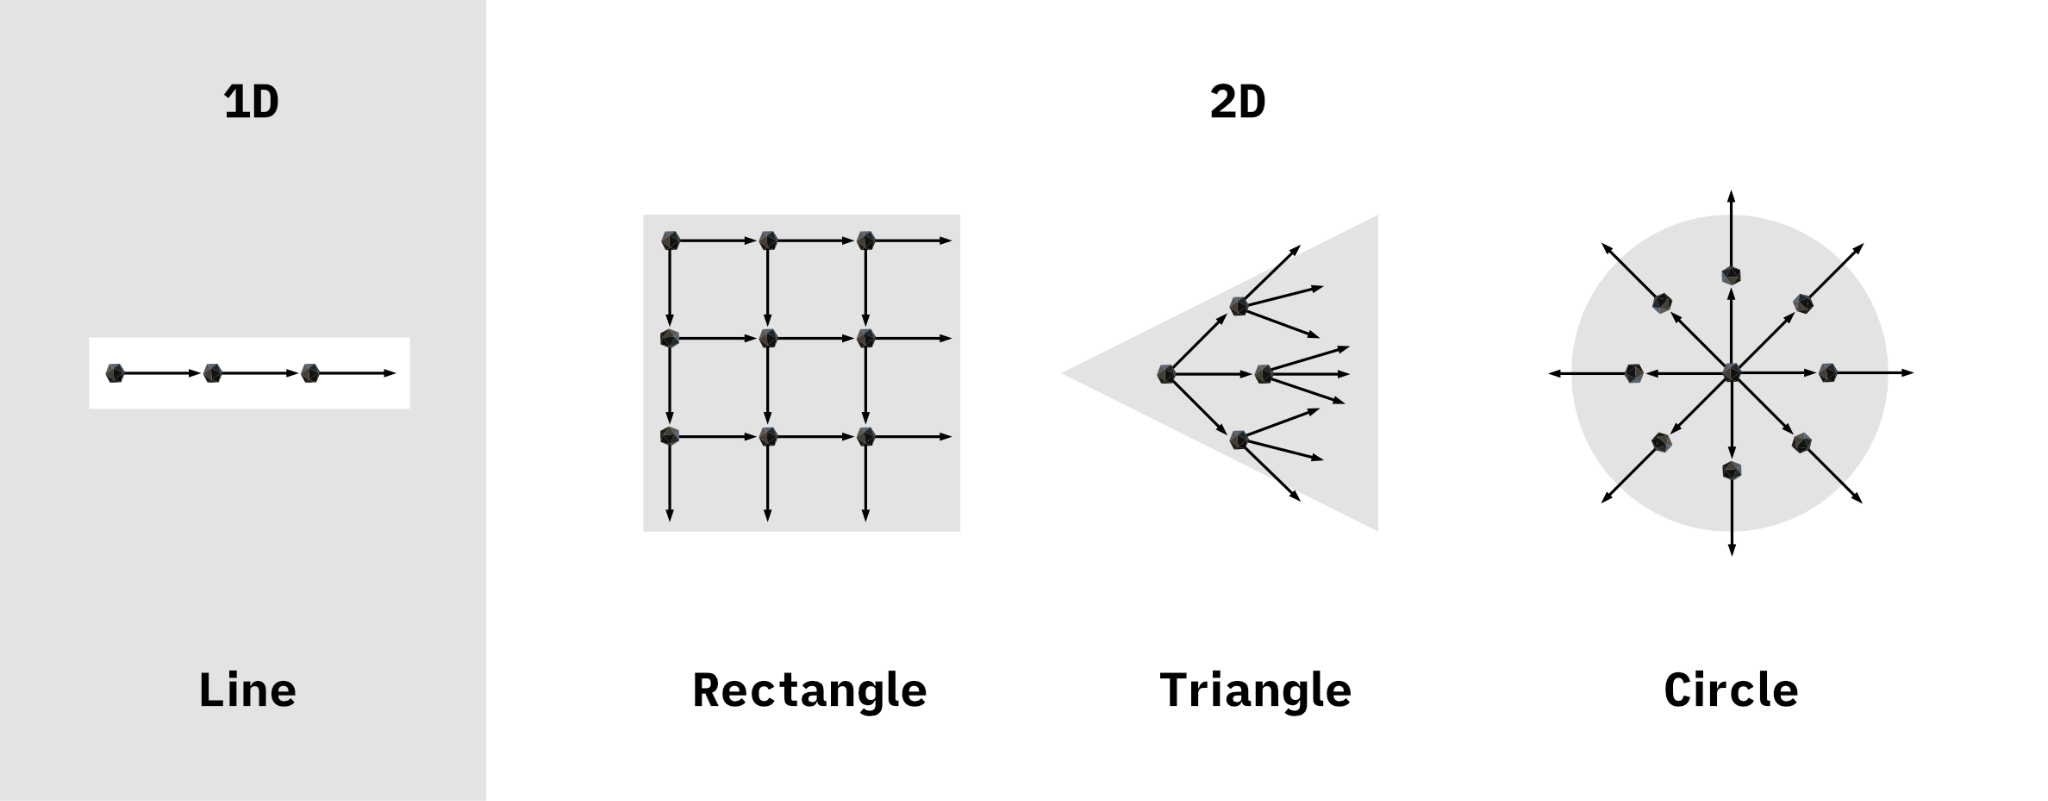
\includegraphics[width=0.8\textwidth]{figures/5.1.png}
    \caption[Network graphs as Semantic Shape]{\textbf{Network graphs as Semantic Shape}. Left: the one-dimensional network graph line. Right: Semantic Shape, two-dimensional network graph radiality compositions: Rectangle, Triangle, and Circle}
    \label{f5.1}
\end{figure}


\begin{figure}[h]
    \centering
    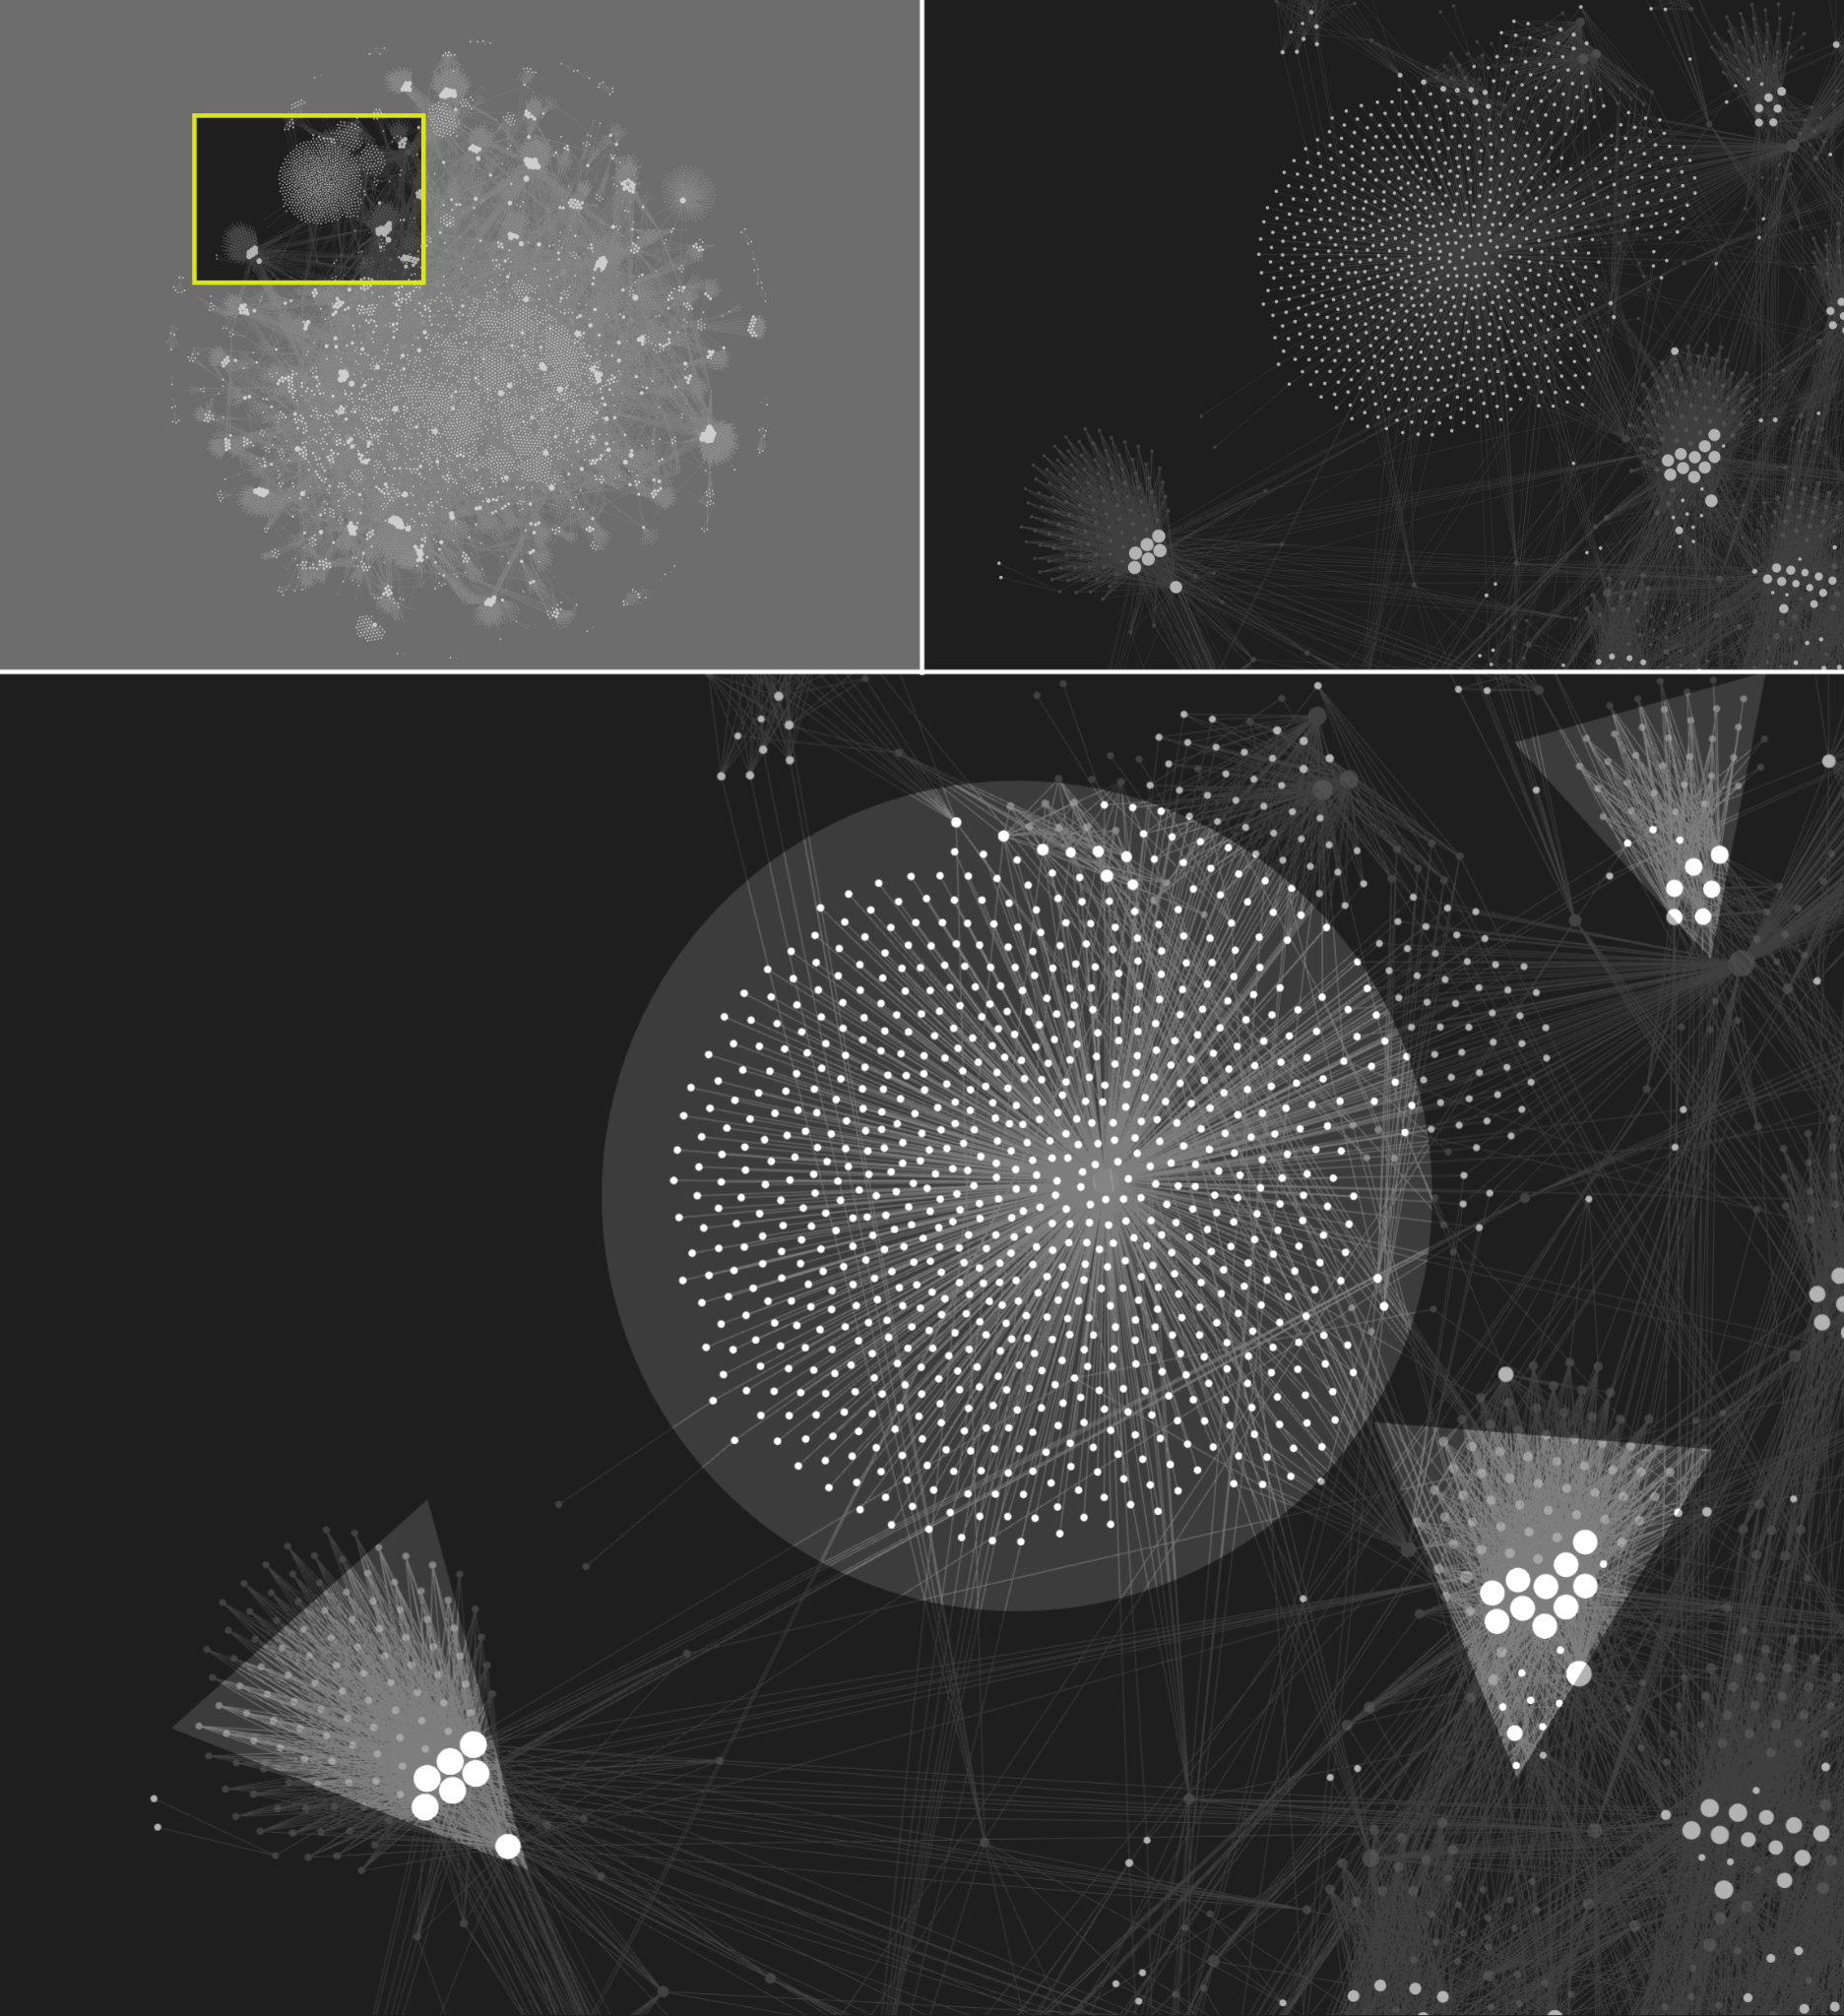
\includegraphics[width=0.8\textwidth]{figures/5.2.png}
    \caption[Example of circle and triangle Semantic Shape nested in a larger Circle Semantic Shape network graph]{\textbf{Example of Circle and Triangle Semantic Shape nested in a larger Circle Semantic Shape network graph.}  \textit{Top left}: Obsidian graph view of my research database; \textit{Top right}: Zoomed view of region marked with yellow-green box. \textit{Bottom}: Labelled Semantic Shape on clusters of network nodes.}
    \label{f5.2}
\end{figure}

\FloatBarrier
%Manuel Lima’s categorization of information visualizations circles and trees \citep{lima_book_2014,lima_book_2017} corroborate the value of my proposal for a Circle Semantic Shape and the triangle Semantic Shape as trees. 

\subsubsection{Semantic Forms: three-dimensional composition types in network graphs}
Moving from one-dimensional network graph lines to two-dimensional network graph Semantic Shape laid the groundwork for adding a third dimension to network graphs and a resulting list of \textit{Semantic Forms}. I approached this exercise as both a deconstruction of complex forms and a combination of Semantic Shape. 
\index[terms]{Semantic Shapes} \index[terms]{Semantic Forms} 

\noindent \textbf{Deconstruction of complex forms}
\\
Calling back to my preceding work involving visualizations of Vedic principles, namely the chakras, perhaps the most pivotal point of my journey from theology into network graphs was through Vedic religious imagery. In particular, two interrelated forms were the object of my delight and fascination: the Sri Yantra and the Meru Chakra. To show my accountability as I strive to honour the religious significance of the Sri Yantra and the Meru Chakra, I have been guided in the study of Vedic spirituality and practice by a number of educators, especially Dr. Monisha Bhatia. However, my work in this thesis with the Sri Yantra and the Meru Chakra will engage their geometric attributes. 
\index[terms]{Sri Yantra} \index[terms]{Meru Chakra} 

Encountering that a two-dimensional graph of lines like the Sri Yantra could interrelate with a three-dimensional visualization like the Meru Chakra encouraged me to consider the opportunities available in dimensional addition to flat graphs. 
\index[terms]{Sri Yantra} \index[terms]{Meru Chakra} 

By averaging out the different steps, or elevations, of the Meru Chakra which has the “the form of a mountain” \citep[p. 31]{buhnemann_mandalas_2003}, the cone form is evident in its composition. The Sri Yantra itself is composed by a central point and its sets of triangles are outlined by a circle. I arrived at the geometric curiosity of a graph of lines that could be represented as both a circle and a cone, the former being more typical of an information visualization composition, and the latter being novel for me as a method for semantic representation of individual elements in a graph. 
\index[terms]{Sri Yantra} \index[terms]{Meru Chakra} 

Upon reflecting on the shape of the horn torus, its two negative spaces within it are shaped like cones. Motivated by this geometric curiosity, I considered how other simple forms could be understood as parts of the horn torus. Following this line of reasoning I arrived at the cylinder as the horn torus’s body, which is also the body of a ring torus. Here, I integrated my preamble work, where I illustrated how a series of horn tori form double-cones. At this point it was easy to envision a horn torus without its double-dimple as a network of nodes organized around a central point, or a sphere. Through this deconstruction process I arrived at a total of six Semantic Forms: the Horn Torus, the Cone, the Ring Torus, the Cylinder, the Sphere, and the Double-Cone. 
\index[terms]{horn torus} 
\index[terms]{ring torus}
\index[terms]{cylinder}
\index[terms]{cone}
\index[terms]{sphere}
\index[terms]{Horn Torus Semantic Form}
\index[terms]{Ring Torus Semantic Form}
\index[terms]{Cylinder Semantic Form}
\index[terms]{Cone Semantic Form}
\index[terms]{Sphere Semantic Form}


\noindent \textbf{Combination of Semantic Shapes}
\\
As a process of combining Semantic Shapes, conversely to the previously explained process of deconstruction, I arrived at the same six Semantic Forms. I illustrate how in \autoref{f5.3}. I begin with the PKM graphs from Obsidian and Logseq a disc-like Circle Semantic Shapes of nodes. I considered the simplest dimensional addition to the Circle, which was to add linear extrusion along a perpendicular axis, creating a Cylinder. I added another form of circular complexity to the Cylinder by circling it in on itself into a Ring Torus. Next, I combined the Triangle and the Circle Semshapes to arrive at the Cone and the Double Cone. Next,  I consider the perpendicular placement of two Circle Semantic Shapes intersecting at their centres by which I arrive at the Sphere. Last, I consider that the Ring Torus can be narrowed to shrink its inner radius to a single point, which makes a Horn Torus.
\clearpage
 \index[terms]{Semantic Shapes} \index[terms]{Semantic Forms} 
 
\FloatBarrier
% First Figure
\begin{figure}[p] % Use [p] to place it on a separate page if needed
    \centering
    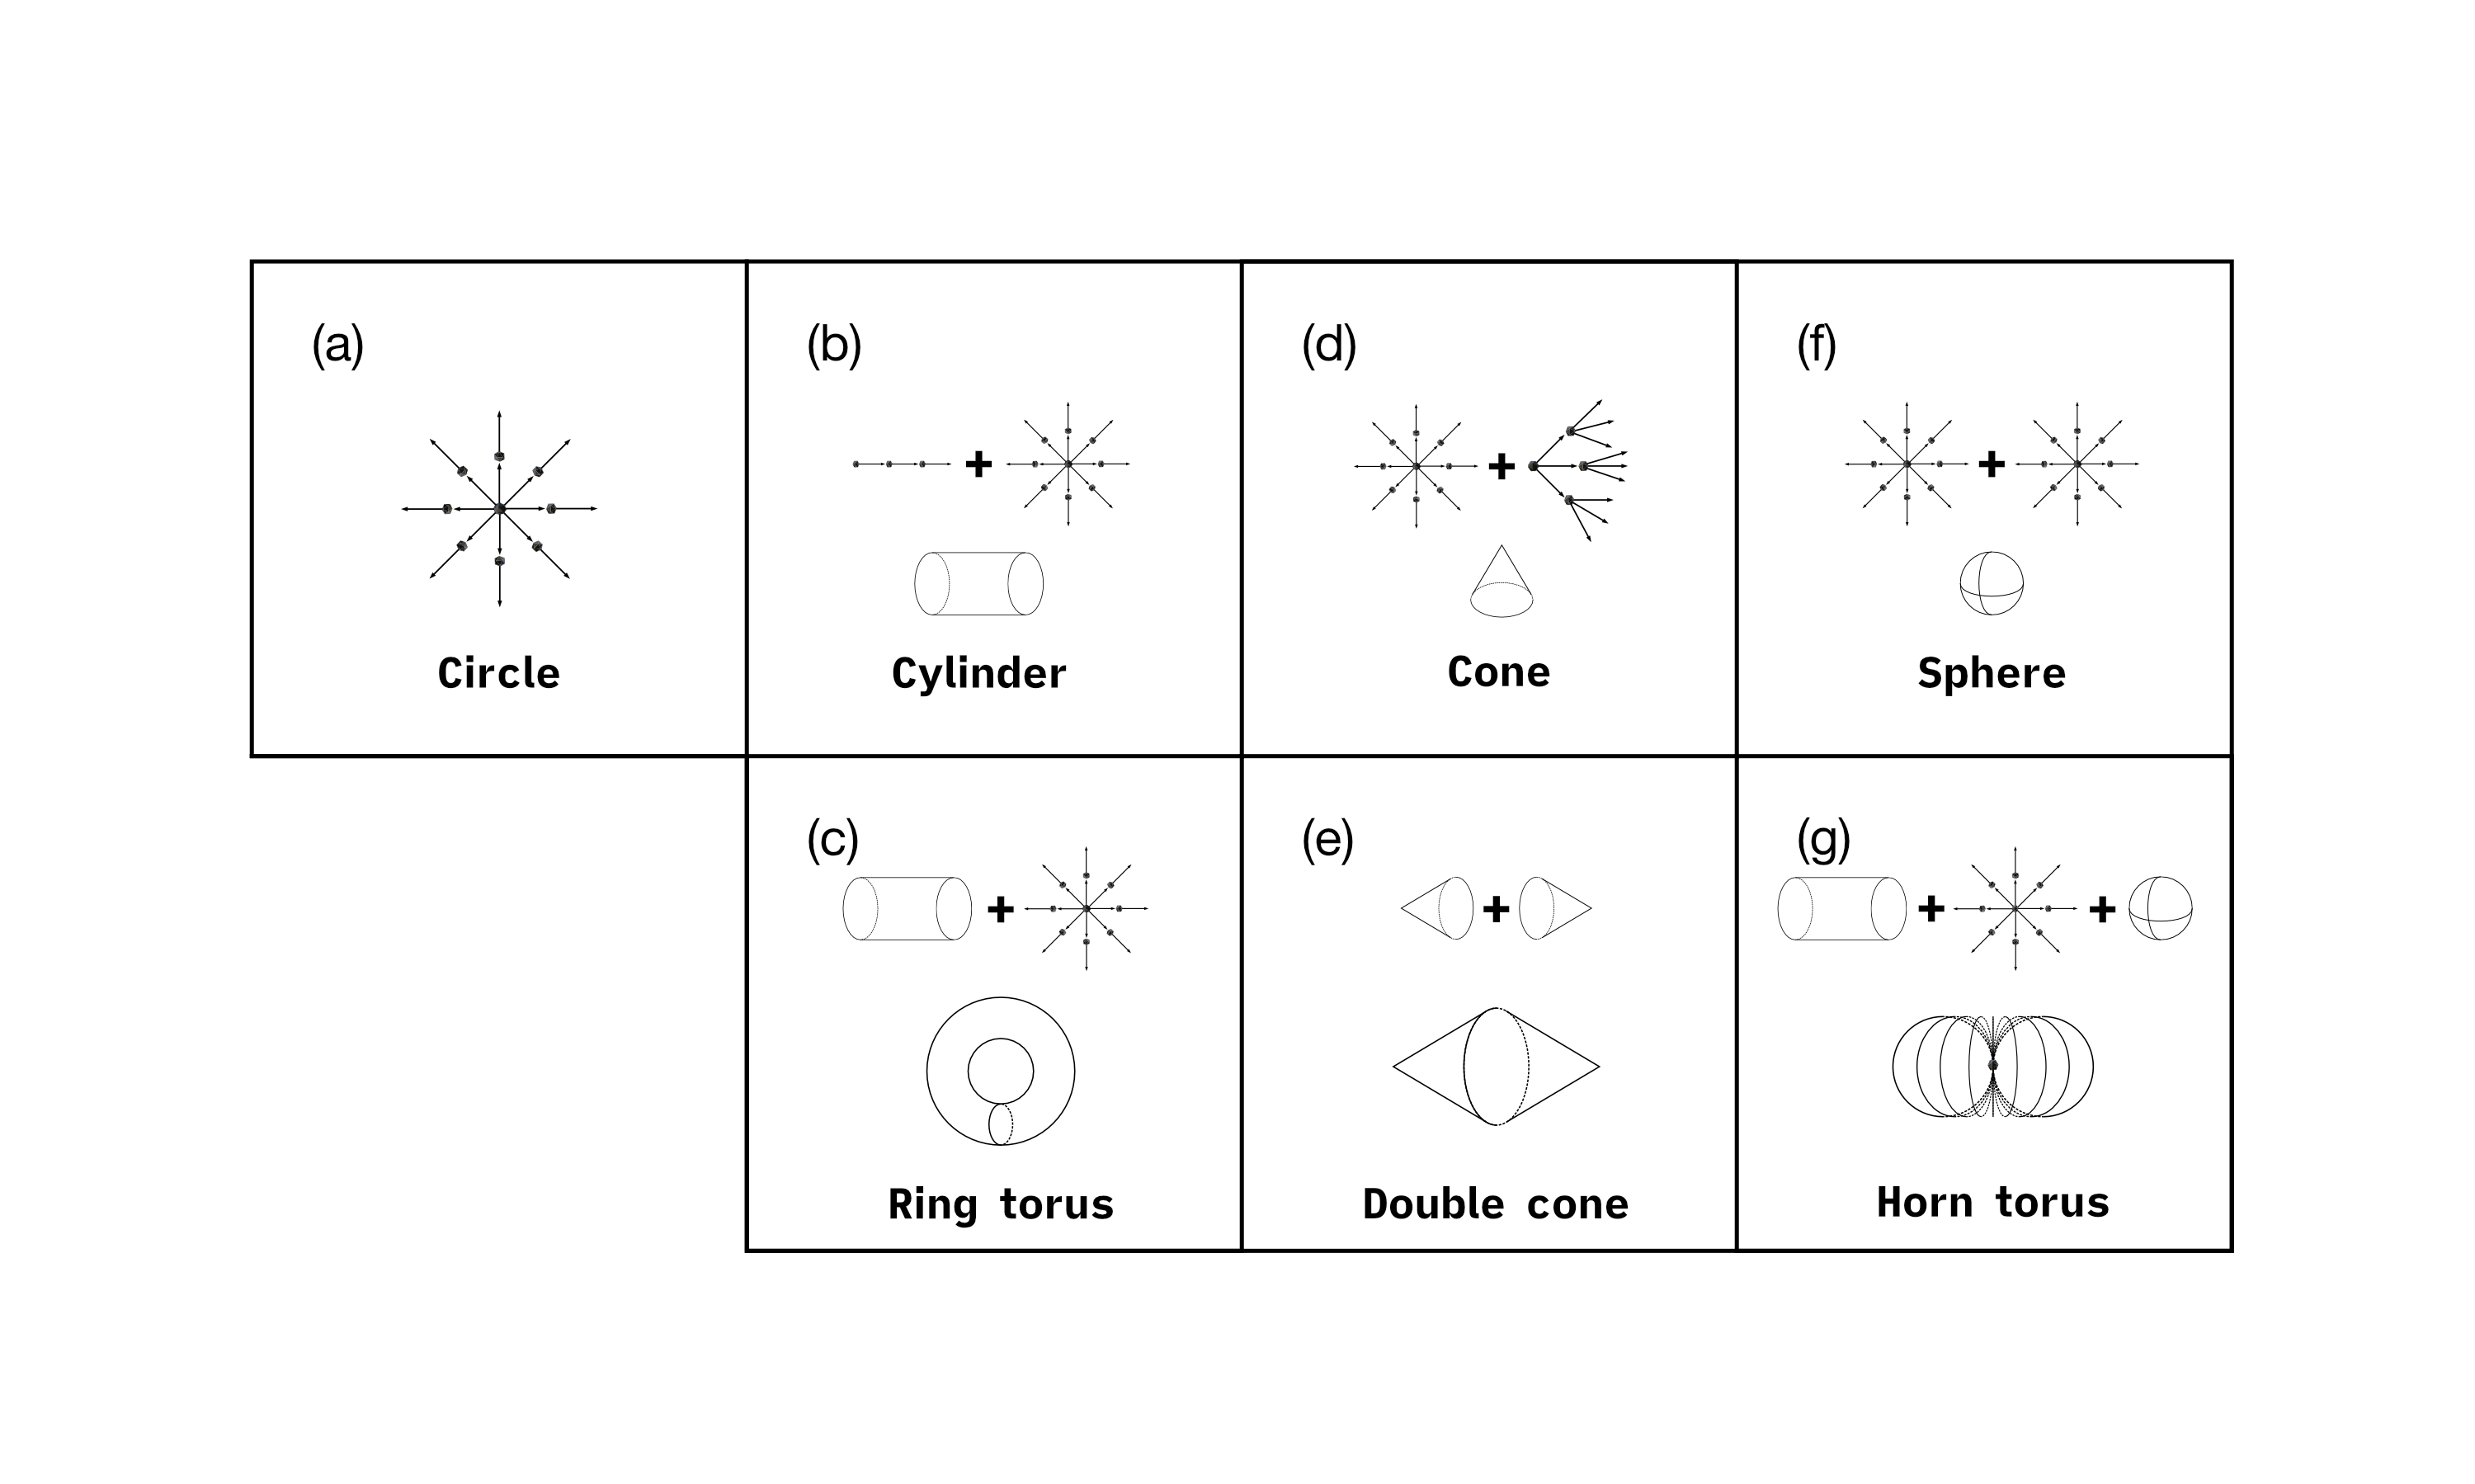
\includegraphics[width=0.8\textwidth]{figures/5.3.png}
    \caption[Semantic Forms derived from the Circle Semantic Shape and other Semantic Forms]
    {\textbf{Semantic Forms} derived from the Circle Semantic Shape and other Semantic Forms. Systematic Combining as dimensional addition to move from two-dimensional to three-dimensional network graph compositions.}
    \label{f5.3}
\end{figure}

% Second Figure
\begin{figure}[p] % Use [p] to place it on a separate page if needed
    \centering
    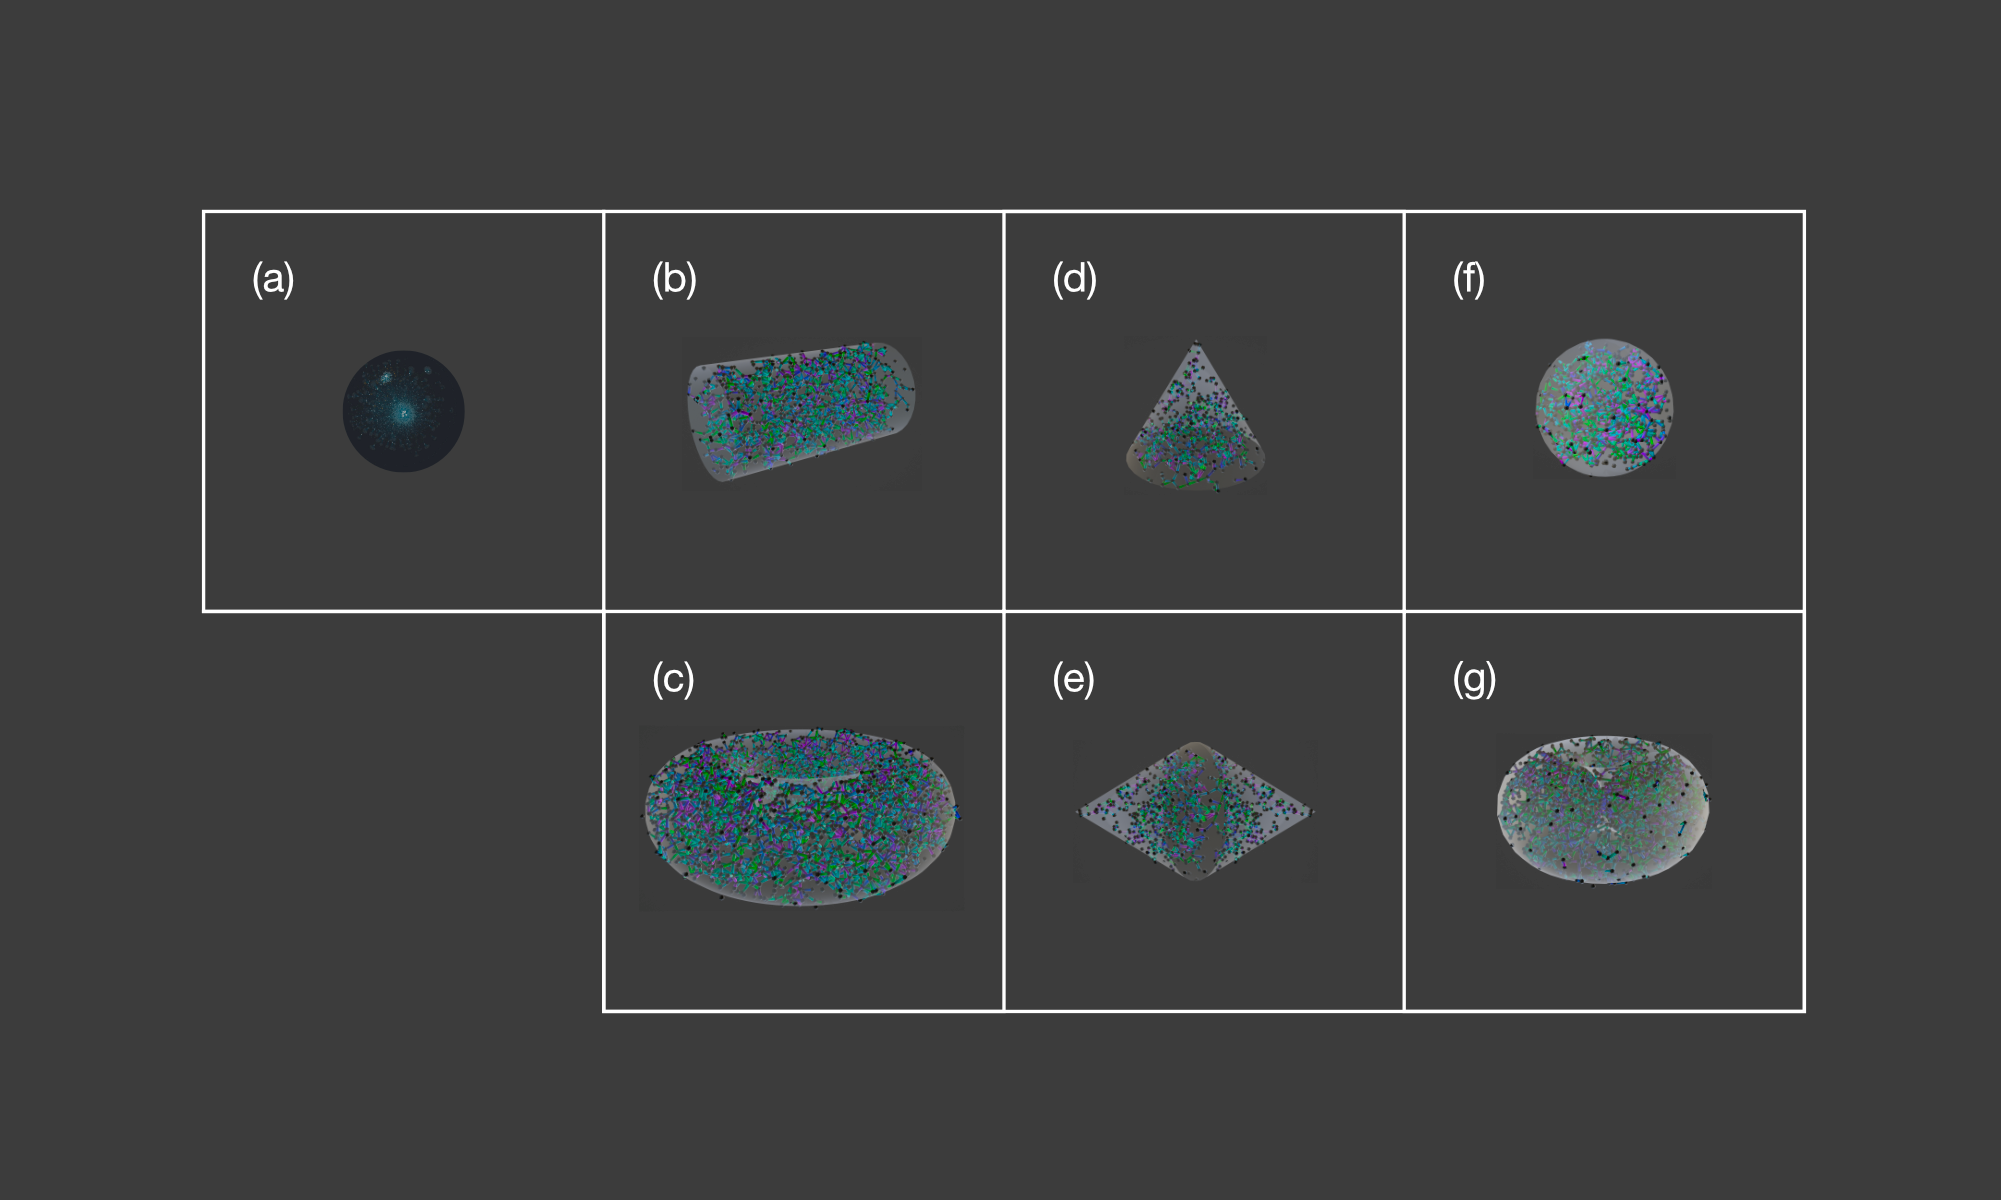
\includegraphics[width=0.8\textwidth]{figures/5.4.png}
       \caption[Knowledge graph disc and six Semantic Forms]{\textbf{Knowledge graph disc and six Semantic Forms}: (a) Circle Semantic Shape knowledge graph, b) Cylinder Semantic Form, (c) Ring Torus Semantic Form, (d) Cone Semantic Form, (e) Double-Cone Semantic Form, (f) Sphere Semantic Form, and (g) Horn Torus Semantic Form. The top row includes more basic forms, and the bottom row includes more geometrically complex ones.}
    \label{f5.4}
\end{figure}
\FloatBarrier
\par





The Semantic Forms are means of three-dimensional hierarchical clustering in a semantic field of terms in a topic model which reveal the semantic relationships like (1) ontological hierarchy of Peircean reasoning modes in which a singular term expresses a general principle and diverse instances of that general principle, (2) cyclicality, and (3) other modes of semantic relationship interpretation in the visuospatial. As a means of capturing hierarchical semantic systems, Semantic Forms have the capacity to nest other Semantic Forms within themselves. In the following section, I illustrate the Semantic Form Cone, Sphere, Cylinder, Cone, Double-Cone, Ring Torus, and Horn Torus.
\index[terms]{Ring Torus Semantic Form}
\index[terms]{Horn Torus Semantic Form}
\index[terms]{Cone Semantic Form}
\index[terms]{Double-Cone Semantic Form}
\index[terms]{Sphere Semantic Form}
\index[terms]{Cylinder Semantic Form}
\index[terms]{Semantic Forms}
\index[people]{Peirce, Charles Sanders}

The \textbf{Cone Semantic Form} is perhaps the most direct illustration of this principle because its form physically turns to a single point. The Sphere Semantic Form encompasses a higher number of radii, which accommodates multiple Cones converging to a single point, or a series of nested convergence points. \autoref{f6.1},\textit{The Ontological Semantic Network Summary of the Syntopicon’s Great Ideas onto the Tree of Porphyry}, is an example of a dimensionally reduced Cone Semantic Form of consilience-oriented information categorization. \autoref{f6.1} demonstrates that Sowa's sense of philosophical-computational ontology and Adler's interdisciplinary term-indexing \citep{adler_great_1952-2} can be understood as a single system through Aristotelian categorization and Porphyrian semantic network graphing \citep[p. 4]{sowa_knowledge_2000}. 
\index[terms]{Syntopicon} \index[terms]{Tree of Porphyry} \index[terms]{Ontological Semantic Network Summary (OSNS)} 
\index[people]{Porphyry}
\index[people]{Sowa, John F.}


The \textbf{Cylinder Semantic Form} provides an extruded space of the flat circular graph and trace individual nodes or graphlets across a third variable along a z-axis, such as time.
\index[terms]{Cylinder Semantic Form} 

The \textbf{Ring Torus Semantic Form} is accommodates the cone as a structure that feeds back to itself in a cycle.
\index[terms]{Ring Torus Semantic Form}

The \textbf{Horn Torus Semantic Form} accommodates multiple cylces that exhibit transformation and feeding back into themselves by emerging from a point, changing, and then returning to that same re-origin point. The horn torus has the distinct ability to nest two Cone-like structures in its negative space as an opportunity for to capture additional semantic interpretation. For instance a moving Horn Torus Semantic Form network graph which is used to topic model a text and identify a re-origin point can also, then, capture the deductive and inductive changes relationships between ideas in that text, or between this given text and other texts.
\index[terms]{Horn Torus Semantic Form} 

Furthermore, The duality represented by two Cones can be used to model the deductive and inductive reasoning in a text or texts. Horn toroidal Semantic Forms will benefit from the overlay of models to compare similar texts and their logical modes. Horn toroidal models can be adapted from static representations to moving models that capture the shifts of reasoning in a given text over time considering its iterations, a set of texts that build on each other, or the representation of popular opinion on a given subject over time. Moving horn toroidal models can, in turn, also be overlaid with each other to compare similar or dissimilar arguments and their corresponding isomorphic Query Isomorph structures.
\index[terms]{Query Isomorph} 


\noindent \textbf{Moving Semantic Forms} 
\\
To render the three-dimensional network graphs of these six Semantic Forms I used Blender to create moving point clouds connected to each other in clusters. Foundational to the node programming required was Manuel Casasola Merkle’s plexus effect tutorial for Entagma \citep{casasola_merkle_blender_2022}.
\index[terms]{Blender} 

The resulting models captured more of my vision for a topic modeling interface that uses three-dimensional network graph Semantic Forms. In terms of information visualization encoding, this software would label categorical and sequential differences between groups of related ideas with colour, and liminal ideas could be identified with colour blends. Moving nodes would represent the changes of a database over time and how some ideas displace and replace others.
\index[terms]{Semantic Forms} \index[terms]{network graph} 

The moving Semantic Form network–as a visualization of computational text analysis like topic modeling, spatial or otherwise–as exemplified in my work, embodies Anderson-Tempini’s isomorphogenesis echoed in Drucker. “We will use the interpretative force of graphical rhetoric as a gesture language of intellectual life, as a way of shaping our communication using the variable dimensions of time and space in ways that print could only hint at, recording as it did the layered, palimpsestic traces of individual and collaborative activities on the enduring substrate of its material surfaces” \citep[p. 197]{drucker_graphesis_2014}. My moving Semantic Form models capture the way in which new information changes the shape of a visuospatial topic model of existing information. For a link to view the moving Semantic Forms see the Appendix.
\index[terms]{isomorphogenesis} \index[terms]{Semantic Forms} 
\index[people]{Drucker, Johanna} \index[people]{Anderson-Tempini, Gemma} 



\noindent \textbf{Geometric analysis}
\\
Upon further geometric investigation of my Semantic Forms, I found that they are closely related to surfaces of revolution, meaning surfaces “generated by rotating a two-dimensional curve about an axis” \citep{weisstein_surface_nodate}. Note the similarities to the Semantic Forms in the following examples: “Examples of surfaces of revolution include the apple surface, cone (excluding the base), conical frustum (excluding the ends), cylinder (excluding the ends), Darwin-de Sitter spheroid, Gabriel's horn, hyperboloid, lemon surface, oblate spheroid, paraboloid, prolate spheroid, pseudosphere, sphere, spheroid, and torus (and its generalization, the toroid)” \citep{weisstein_surface_nodate}.
\index[terms]{torus} 
\index[terms]{surfaces of revolution} 
\index[terms]{Semantic Forms} 
\index[terms]{Personal Knowledge Management (PKM)} 
\index[terms]{Ring Torus Semantic Form}
\index[terms]{Sphere Semantic Form}

When considering the combination of Semantic Shapes I was more concerned about new forms of spatial network graph plotting \textit{into} the Semantic Forms, so I did not originally consider the Semantic Forms' surfaces as their own classifications.

I suspect considering Semantic Forms in relation to surfaces of rotation will yield new forms for network graph plotting. To begin the differentiation of the Semantic Forms’ volume and surface for the next steps of their geometric analysis, I list the Semantic Forms’ volume and surface equations in Cartesian coordinates as a starting point in Appendix \autoref{Semantic Forms equations}, though spherical coordinates may be more suited for further azimuthal analysis.

\index[terms]{torus} 
\index[terms]{surfaces of revolution} 
\index[terms]{Semantic Forms} 
\index[terms]{Personal Knowledge Management (PKM)} 
\index[terms]{Ring Torus Semantic Form}
\index[terms]{Sphere Semantic Form}

\noindent \textbf{Tidiness of the Semantic Form models}
\\
While I am observing the geometry of such compositions and providing examples that neatly showcase their shapes and forms, I am not claiming to advocate for node-by-node retrofitting to fit these models, which would be a disservice to the data. Finding patterns in data is difficult in two dimensions, let alone any dimensions above it. In future work, I will examine the various mathematical approaches to identifying Semantic Form patterns in large network models of computationally modeled data. The focus of this work is to identify the semantic value of an array of shapes and forms so as to establish which patterns to look for. The finding of these patterns in real data is for another work. \\

By making Semantic Forms I sought to define the ways geometric form can be given topological versatility in the ways large groups of nodes reveal group semantic relationships, similar to Global Topological Synchronization \citep{wang_global_2024,bianconi_topology_2024}. In the following section I aim to focus on the smaller network chunks within these more macroscopic murmurations. 
\index[terms]{Semantic Forms} \index[terms]{Global Topological Synchronization (GTS)} 





\section{Contribution 2: Query Isomorphs}
\begin{enumerate}
        \item[\textbf{C2}] \textit{Query Isomorphs} as a means of Topological Capta Analysis (TCA) in HITL CATG using small graph chunks.
\end{enumerate}


\subsection{Defining the Query Isomorph}

I propose Query Isomorphs or isomorphic directed graphlets as two-and-three-dimensional query object and query interface. Query Isomorphs differ from Sowa's query, conceptual, and canonical graphs, in their dimensional versatility using Topological Capta Analysis. TCA supports models and queries across any number of dimensions, and certainly within the visible three dimensions, including moving Semantic Form graphs. \footnote{As a point to refer to more contemporary applications of querying using graphs, it is worth noting developments that use AI. TerminusDB’s platform is evidence of semantic isomorphology} querying using AI. Their vector search is an example of how querying vectors enables “efficient and accurate similarity-based querying” and “clustering algorithms to gain valuable insights from massive datasets” as a means to “model data in a more semantically meaningful manner, enabling a deeper understanding of the connections between different entities” This study did not engage with TerminusDB graphs because they are high-dimensional and do not reveal their process within the visible three dimensions. \citep{terminusdb_enterprise_2023}.
\index[terms]{Query Isomorphs} 
\index[people]{Sowa, John F.}

Canonical graphs \citep[p. 53]{sowa_semantics_2013} are related to my Query Isomorphs in that they can help recognize patterns of meaning across different texts and contexts to facilitate faster KSSTC. Query Isomorphs differ from canonical graphs  \citep[p. 53]{sowa_semantics_2013}, as well as query graphs \citep[p. 313]{sowa_conceptual_1984} and conceptual graphs \citep[p. 53]{sowa_semantics_2013}, as \textit{dimensionally versatile} elements queriable with TDA and TCA. Query Isomorphs can themselves be dimensionally versatile \textit{query interface} in one, two, or three dimensions (with or without movement). I arrived at my own ideas of isomorphological query graphlets independently from Sowa, but considering my work stands in his legacy I choose to include the word ‘Query’ in Query Isomorph in honour of his query graphs. 
\index[terms]{Query Isomorphs} 

Isomorphology has a wider application than Anderson-Tempini \citep{anderson_drawing_2018}. and Even Gothe \citep[p. 11]{anderson_drawing_2018} which includes chemistry.The ways molecules of a given element or elements maintain repeatable configurations of atom-bond relationships is also isomorphology. I considered naming Query Isomorphs 'datacules' for this reason. However, in this thesis I align my graphlet thought experiment with Drucker's humanistic design. Drucker asserts that ``\textit{data are capta}, taken not given, constructed as an interpretation of the phenomenal world, not inherent in it." \citep[p. 128]{drucker_graphesis_2014}. I propose that isomorphology reveals what Drucker refers to as the ``constructedness of data as capta" \citep[p. 128]{drucker_graphesis_2014}. Considering the versatility of isomorphology across disciplines I chose it as one of my neologism’s key identifiers. This is the ‘Isomorph’ in Query Isomorph.

\noindent \textbf{Semantic Field \textit{S} and Sample \textit{s}}
\\
In the following section I will illustrate an example Query Isomorph. But, no term exists in isolation so first I will introduce the semantic field \citep[p. 107]{jurafsky_speech_2024} which contextualizes my Query Isomorph example. In this section I introduce a sample of terms from the semantic field of this thesis, which I call Sample \textit{s}. The larger set of 312 terms, Semantic Field \textit{S}, is included in my Appendix.


Sample \textit{s} is a list of nineteen ideas which I arbitrarily selected from Semantic Field \textit{S} for having high importance in my thesis. In \autoref{tab:semantic_fields} I list the terms from Sample \textit{s} along with the date of their earliest recorded use, and a note of where the idea was first recorded. I use the word idea here and not term because some terms have changed over time. For example Query Isomorph was first ‘datacule’ as mentioned previously. The idea remains the same, but the term is different. 



\begin{table}[htbp]
  \centering
  \begin{tabular}{p{0.4cm}p{4cm}p{2.5cm}p{5cm}}
      \toprule
      \textbf{\#} & \textbf{Sample \textit{s} term} & \textbf{Earliest use on record} & \textbf{Note} \\
      \midrule
      1 & Symbol-making & 2022 Jan and earlier & Prior studies: note-taking methods experimentation \\
      2 & Sri Yantra & 2022 Jan and earlier & Prior studies: theology \\
      3 & Network Graphs & 2022 Jan and earlier & Prior studies: note-taking methods \\
      4 & Meru Chakra & 2022 Jan and earlier & Prior studies: theology \\
      5 & Personal Knowledge Management (PKM) & 2022 Jan 12 & Obsidian: first vault \\
      6 & Torus & 2022 Mar 17 & Images: RSF Torus Yin-Yang \\
      7 & Graphesis & 2022 May 01 & Images: Drucker (2014) first read \\
      8 & Isomorphology & 2022 Jun 21 & Images: Anderson-Tempini (2018) first read \\
      9 & Topology & 2022 Nov 22 & Logseq: Adam Tindale meeting notes \\
      10 & Spatial Information Visualization Composition (SIVC) & 2022 Nov 30 & Logseq: Saint-Martin (1990) first read \\
      11 & Semantic Forms & 2023 Jul 31 & Physical notebooks: first sketches of Semantic Forms \\
      12 & Query Isomorphs  & 2023 Aug 06 & Physical notebooks: first sketches of the Query Isomorph, then called 'Datacules' \\
      13 & Topic Models & 2023 Jul 11 & Zotero: InfraNodus added \\
      14 & Gigamapping & 2023 Sep 28 & Zotero: Sevaldson (2022) added  \\
      15 & Systematic Combining & 2024 Apr 17 & Zotero: Kjøde (2024) added \\
      16 & Persistence Homology (PH) & 2024 Jun 10 & Watched Bianconi's talk at the IDEAS Research Centre \\
      17 & Global Topological Synchronization (GTS) & 2024 Jul 15 & Wang et al. added to Zotero \\
      18 & Computational Semiosis & 2024 Oct 15 & New term: expansion of Computational Graphesis \\
      19 & TCA & 2024 Oct 30 & New term: information-oriented differentiation from TDA \\
      \bottomrule
  \end{tabular}
  \caption{Sample \textit{s} terms chronology}
  \label{tab:semantic_fields}
\end{table}
\index[terms]{gigamapping}


\subsubsection{Visualization style for the Query Isomorph}
At this point in the document I will begin using three-dimensional objects made in Blender. I decided to keep the dark grey background typical of the Blender platform in alignment with Drucker's sense of humanist post-structuralist design, which reveals the ``constructedness of knowledge" \citep[p. 178]{drucker_graphesis_2014} in visuospatial forms of ``knowledge production" \citep{drucker_graphesis_2014}. I used the shape of a Blender icosphere as the form of each node to refer back to the spatial interface I intend for Query Isomorphs to be use in. 
\index[people]{Drucker, Johanna}

To design my figures I draw from \textit{Spectrum}, Adobe's design system, and its guide, \textit{Color for data visualization} \citep{adobe_color_2022}. I use its categorical colour palette to represent differences between ideas that operate in different semantic lanes. For example, the difference between words more closely associated with Semantic Forms, as opposed to the words more closely associated with Query Isomorphs.
 
I use the Adobe \textit{Spectrum} sequential colour palette \citep{adobe_color_2022} to represent ideas that are incrementally different along a semantic spectrum. For example, the gradiating difference between the highly summative$/$less numerous terms like ``Computational Semiosis", and less summative$/$more numerous terms like ``Isomorphology" and ``Topic models".  

I chose the colour of the edges in my moving Semantic Form network graphs to gradiate across the indigo-teal-green continuum in general alignment with the Viridis sequential colour palette. The use of gradient, instead of isolated hues separated from a continuum, represents the subtle semantic gradiation between related ideas in the topic model of a complex text. 

When iterating my graphs, the more complex illustrations include three sequential colours and three or more categorical colours. In practice, these more complex figures required a lighter colour for the lightest sequential figures. I tested a colour from the same Adobe Spectrum \textit{Color for data visualization} \citep{adobe_color_2022}, specifically the middle colour of its diverging colour palettes, \texttt{\#FFFFE0} (Light yellow). 

In practical application Light yellow was difficult to distinguish from white annotations like axes lines. I tested options for colour options darker than Light yellow colour slightly while keeping it substantially lighter than light green, and arrived at \texttt{\#FFF7C7} (Lemon chiffon). 

As a result, my figure illustration style guide consisted of four categorical colours and three sequential colours. The categorical colours are: \texttt{\#0FB5AE} (Seafoam 600), \texttt{\#F68511} (Orange 600), \texttt{\#DE3D82} (Magenta 800), \texttt{\#7E84FA} (similar to Indigo 700). For simplicity of description of the illustrations that follow, I will refer to these as the categorical figure colours Teal, Orange, Magenta, and Purple. The sequential figure colours are: \texttt{\#FFF7C7} (Lemon chiffon)), \texttt{\#D2E21B} (Pear), and \texttt{\#7AD151} (Atlantis) to designate high, middle, and low summativeness respectively. I will refer to these as the sequential figure colours Light yellow, Light green, and Green.
\footnote{Categorical figure colours were not assigned word names by Adobe in \textit{Spectrum}\citep{adobe_color_2022} in addition to their hexcodes, so I included the name provided by the Colblindor Color Name \& Hue tool \citep{fluck_color_2021}.}

I ensured that the colours I chose for my design system adhere to the Adobe Color Blind Safe color checker \citep{adobe_accessibility_2024}. I confirmed that the contrast ratio is higher than the minimum required 3:1 ratio for all colours used using WCAG 2.2 Technique G183 \citep{world_wide_web_consortium_w3c_technique_2024}.



\FloatBarrier   
\begin{figure}[h!]
    \centering
    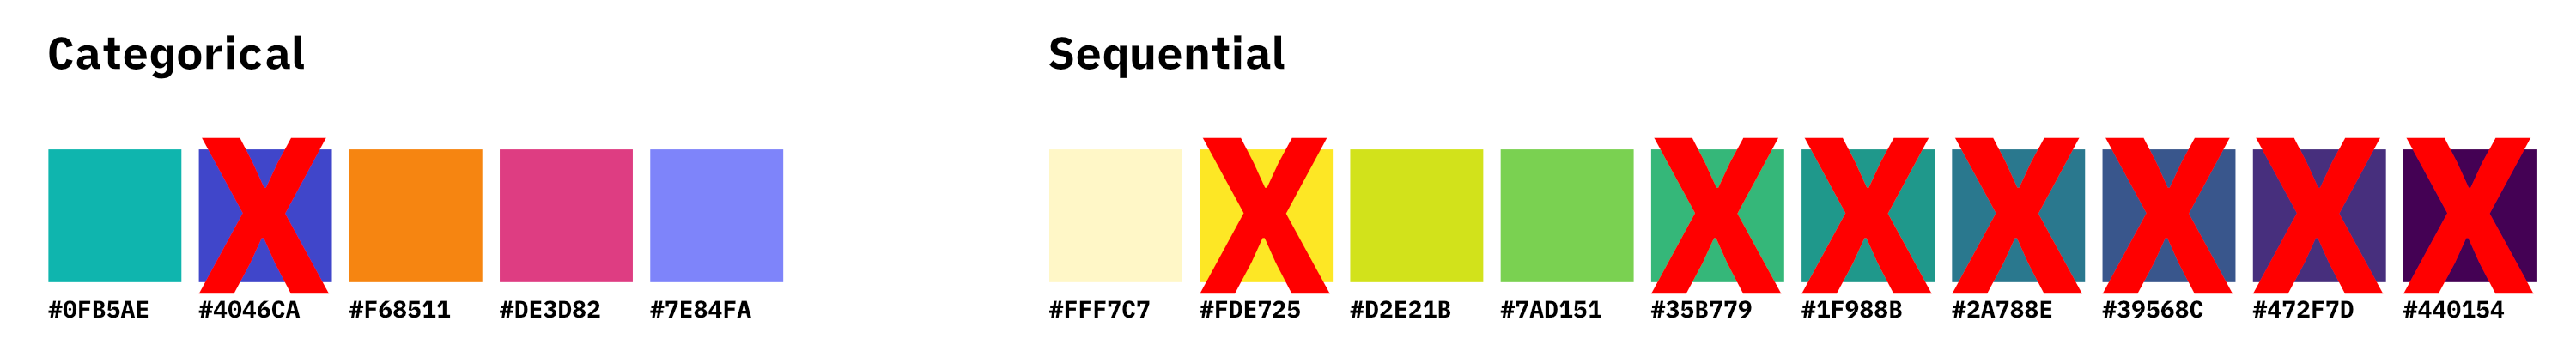
\includegraphics[width=\textwidth]{figures/5 considered.png}
    \caption[Colours considered]{\textbf{Colours considered} from the Adobe Spectrum design system \textit{Color for data visualization} \citep{adobe_color_2022}.}
    \label{5 considered}
\end{figure}

\begin{figure}[h!]
    \centering
    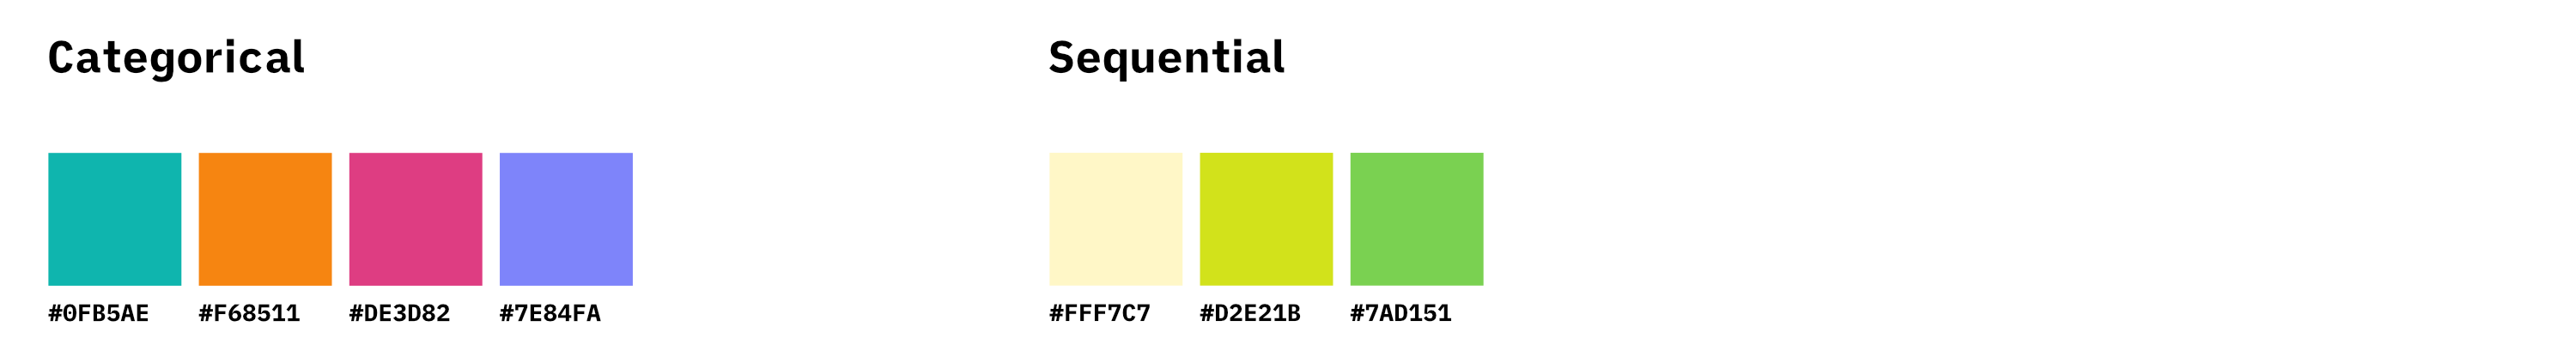
\includegraphics[width=\textwidth]{figures/5 selected.png}
    \caption[Colours chosen]{\textbf{Colours chosen} from the Adobe Spectrum design system \textit{Color for data visualization} \citep{adobe_color_2022}.}
    \label{5 selected}
\end{figure}
\FloatBarrier  

\noindent \textbf{Illustrating Sample \textit{s} as network nodes}
\\

To apply this visualization style to \autoref{tab:semantic_fields} \autoref{f5.11.Sample s} visualizes each idea as a node paired with its label. I have arbitrarily designated each node-label pairing as a high-summative node, mid-summative node, or a low-summative node respectively labelled as Light yellow, Light green, or green, as per my chosen set of sequential figure colours. On the left I list all nineteen ideas from Sample \textit{s}, and on the right I list the nodes I will use in illustrations of Query Isomorph \textit{i}. Neologisms have a tilde beside them (~), and Contributions have an asterisk beside them (*). Note that the names I gave my contributions are also neologisms, so they have both a tilde (~) and an asterisk (*) shown as ~*.


\begin{figure}[h!]
    \centering
    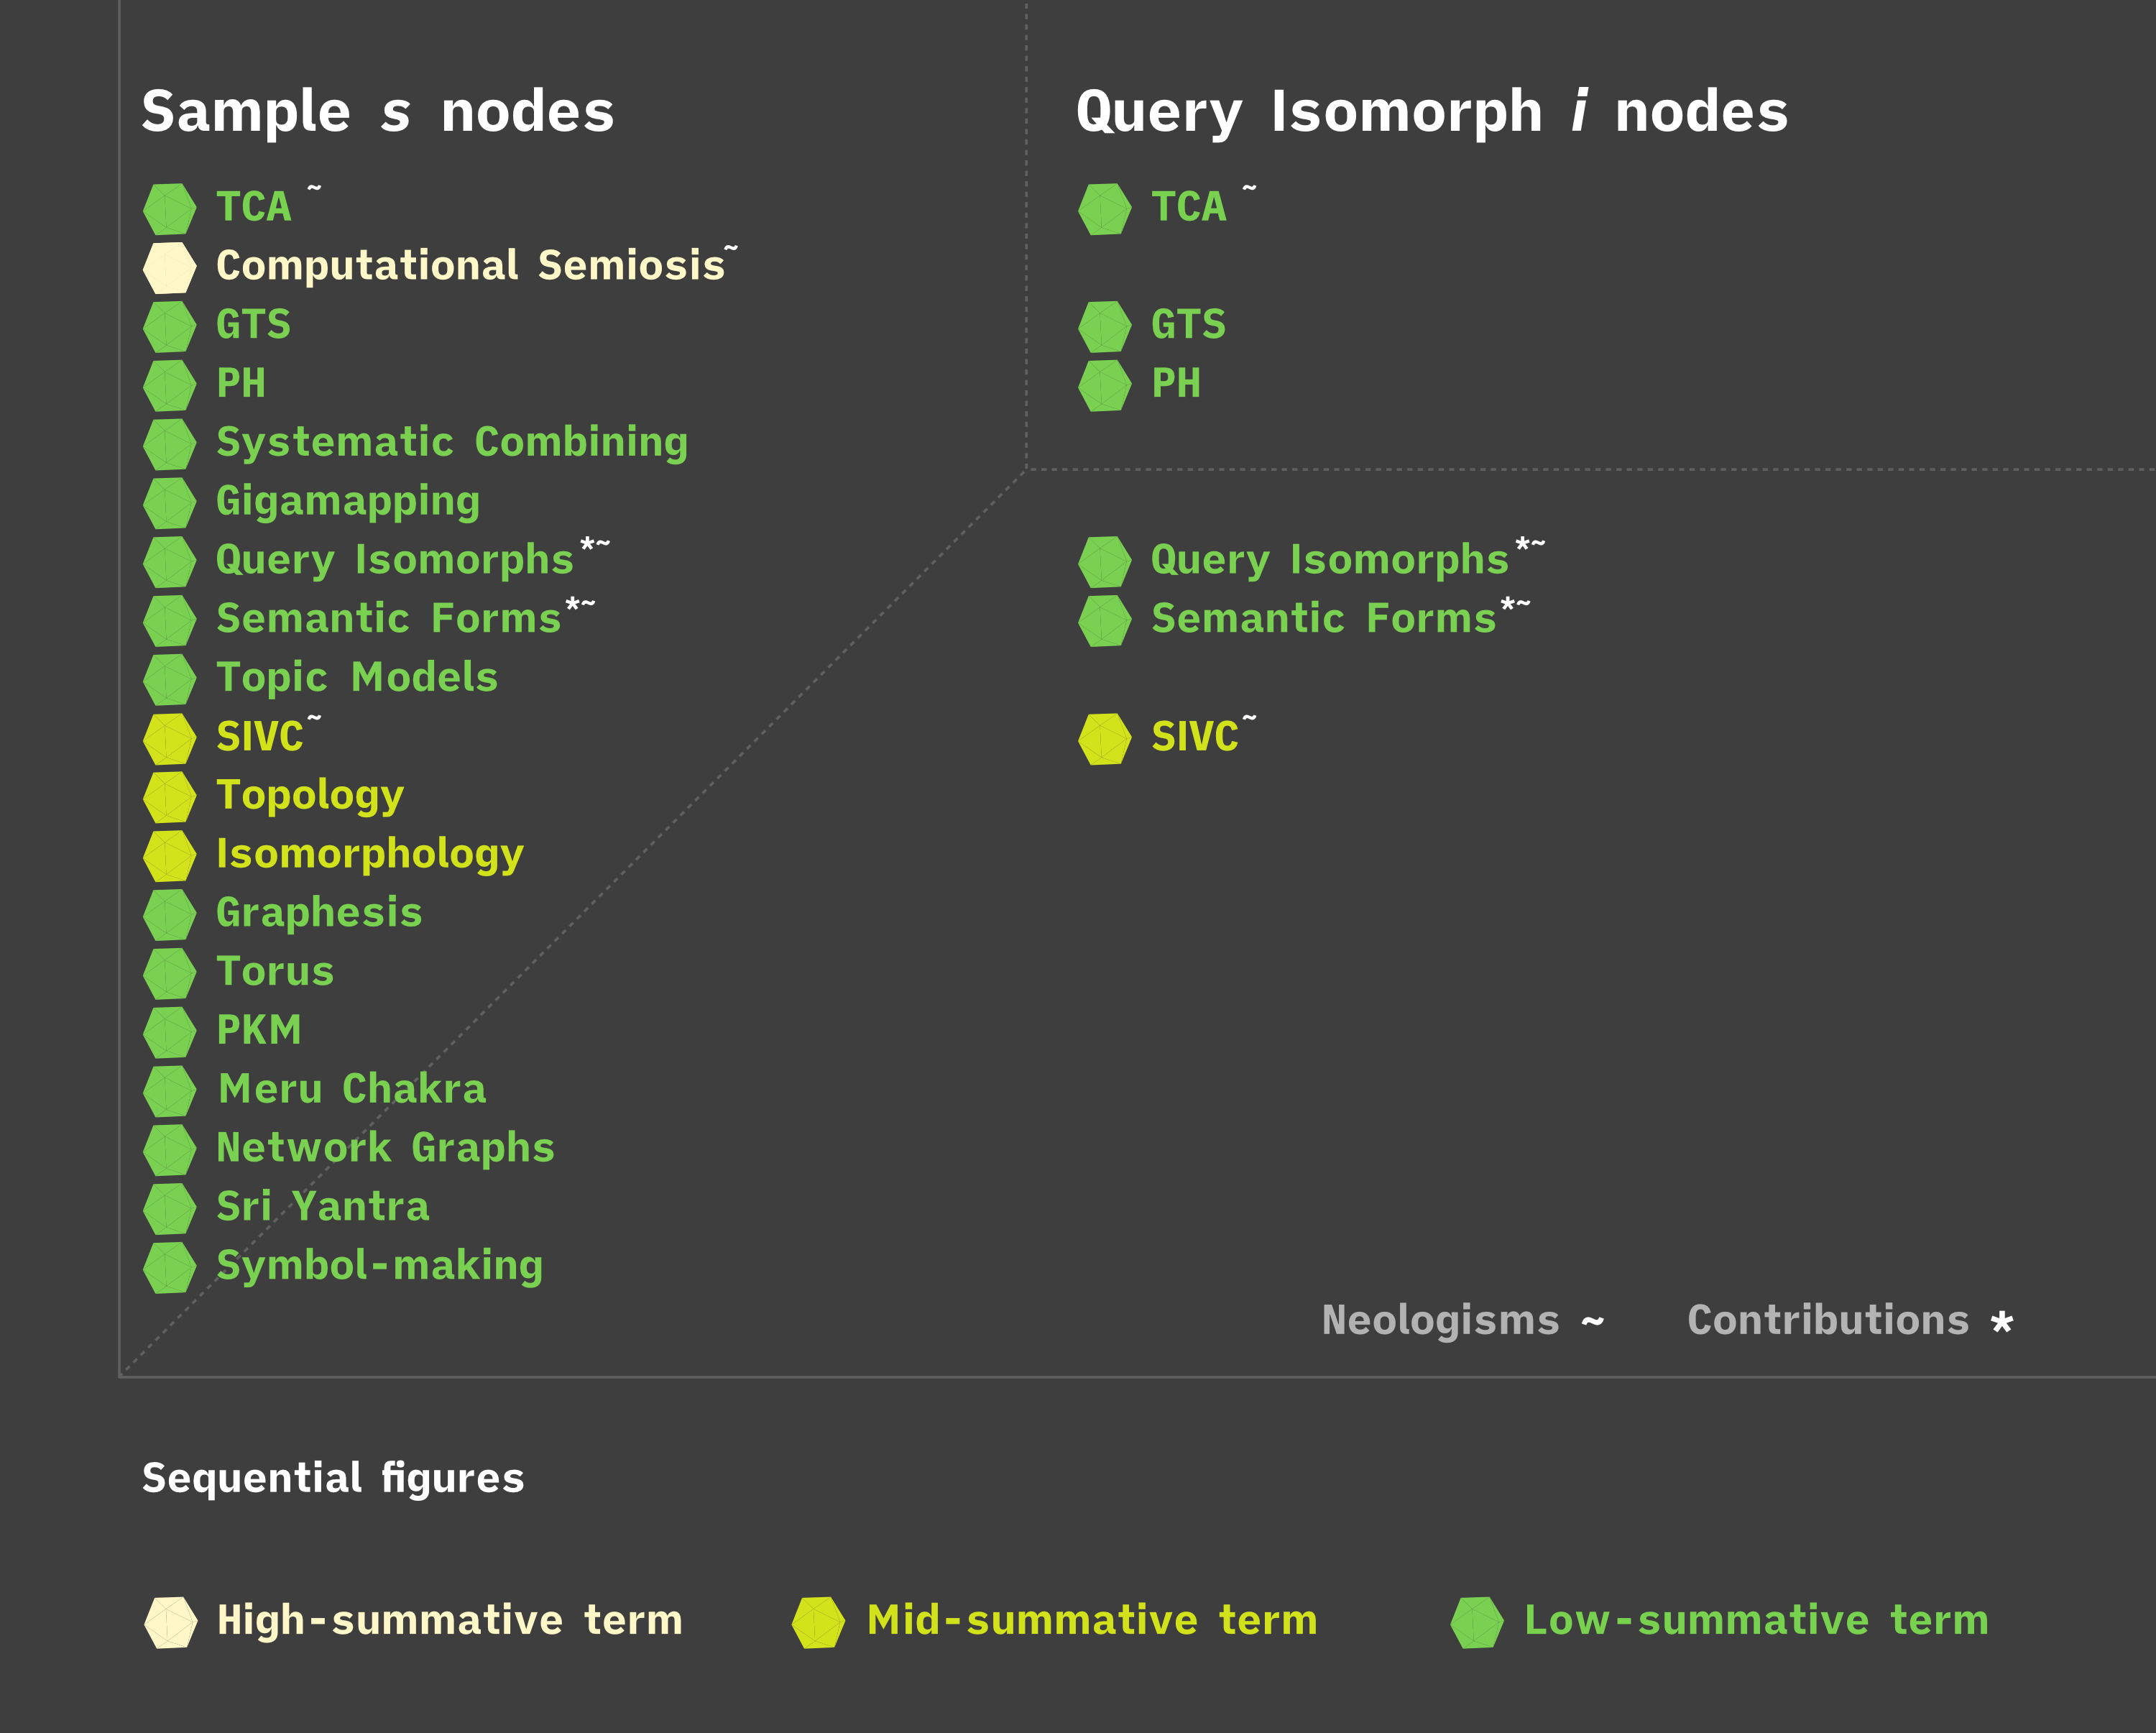
\includegraphics[width=0.7\textwidth]{figures/5.11.Sample s.png}
    \caption[Sample \textit{s} ideas list and Query Isomorph \textit{i} ideas list]{\textbf{Sample \textit{s} ideas list and Query Isomorph \textit{i} ideas list.}}
    \label{f5.11.Sample s}
\end{figure}


\noindent \textbf{\textit{Timelines of Sample \textit{s} terms}}
\\

\autoref{f5.11.Time line} illustrates when each idea was first included in my research database on a linear timeline. The purpose of including this timeline is to visualize the time that has passed between the inclusion of each idea in Sample \textit{s}. This figure also introduces some key design components for illustrations of my example Query Isomorph which follow later in this section. Note that terms are paired with a node, which will be instrumental to illustrate spatial node relationships. Also note that nodes and text are labelled with sequential figure colours for high-summative, mid-summative and low-summative term nodes. This illustration also includes the date and origin note from \autoref{tab:semantic_fields}. Some Semantic Forms are arranged using rectileaner timelines, like the Cylinder. 

Not all Semantic Forms use rectilinear time representations, the Ring Torus for example. To accommodate cycles of time represented as ellipses, I transposed \autoref{f5.11.Time line}, the Linear Timeline of terms of Sample\textit{s}, onto the circumference of a circle. 

\FloatBarrier  
\begin{figure}[h!]
    \centering
    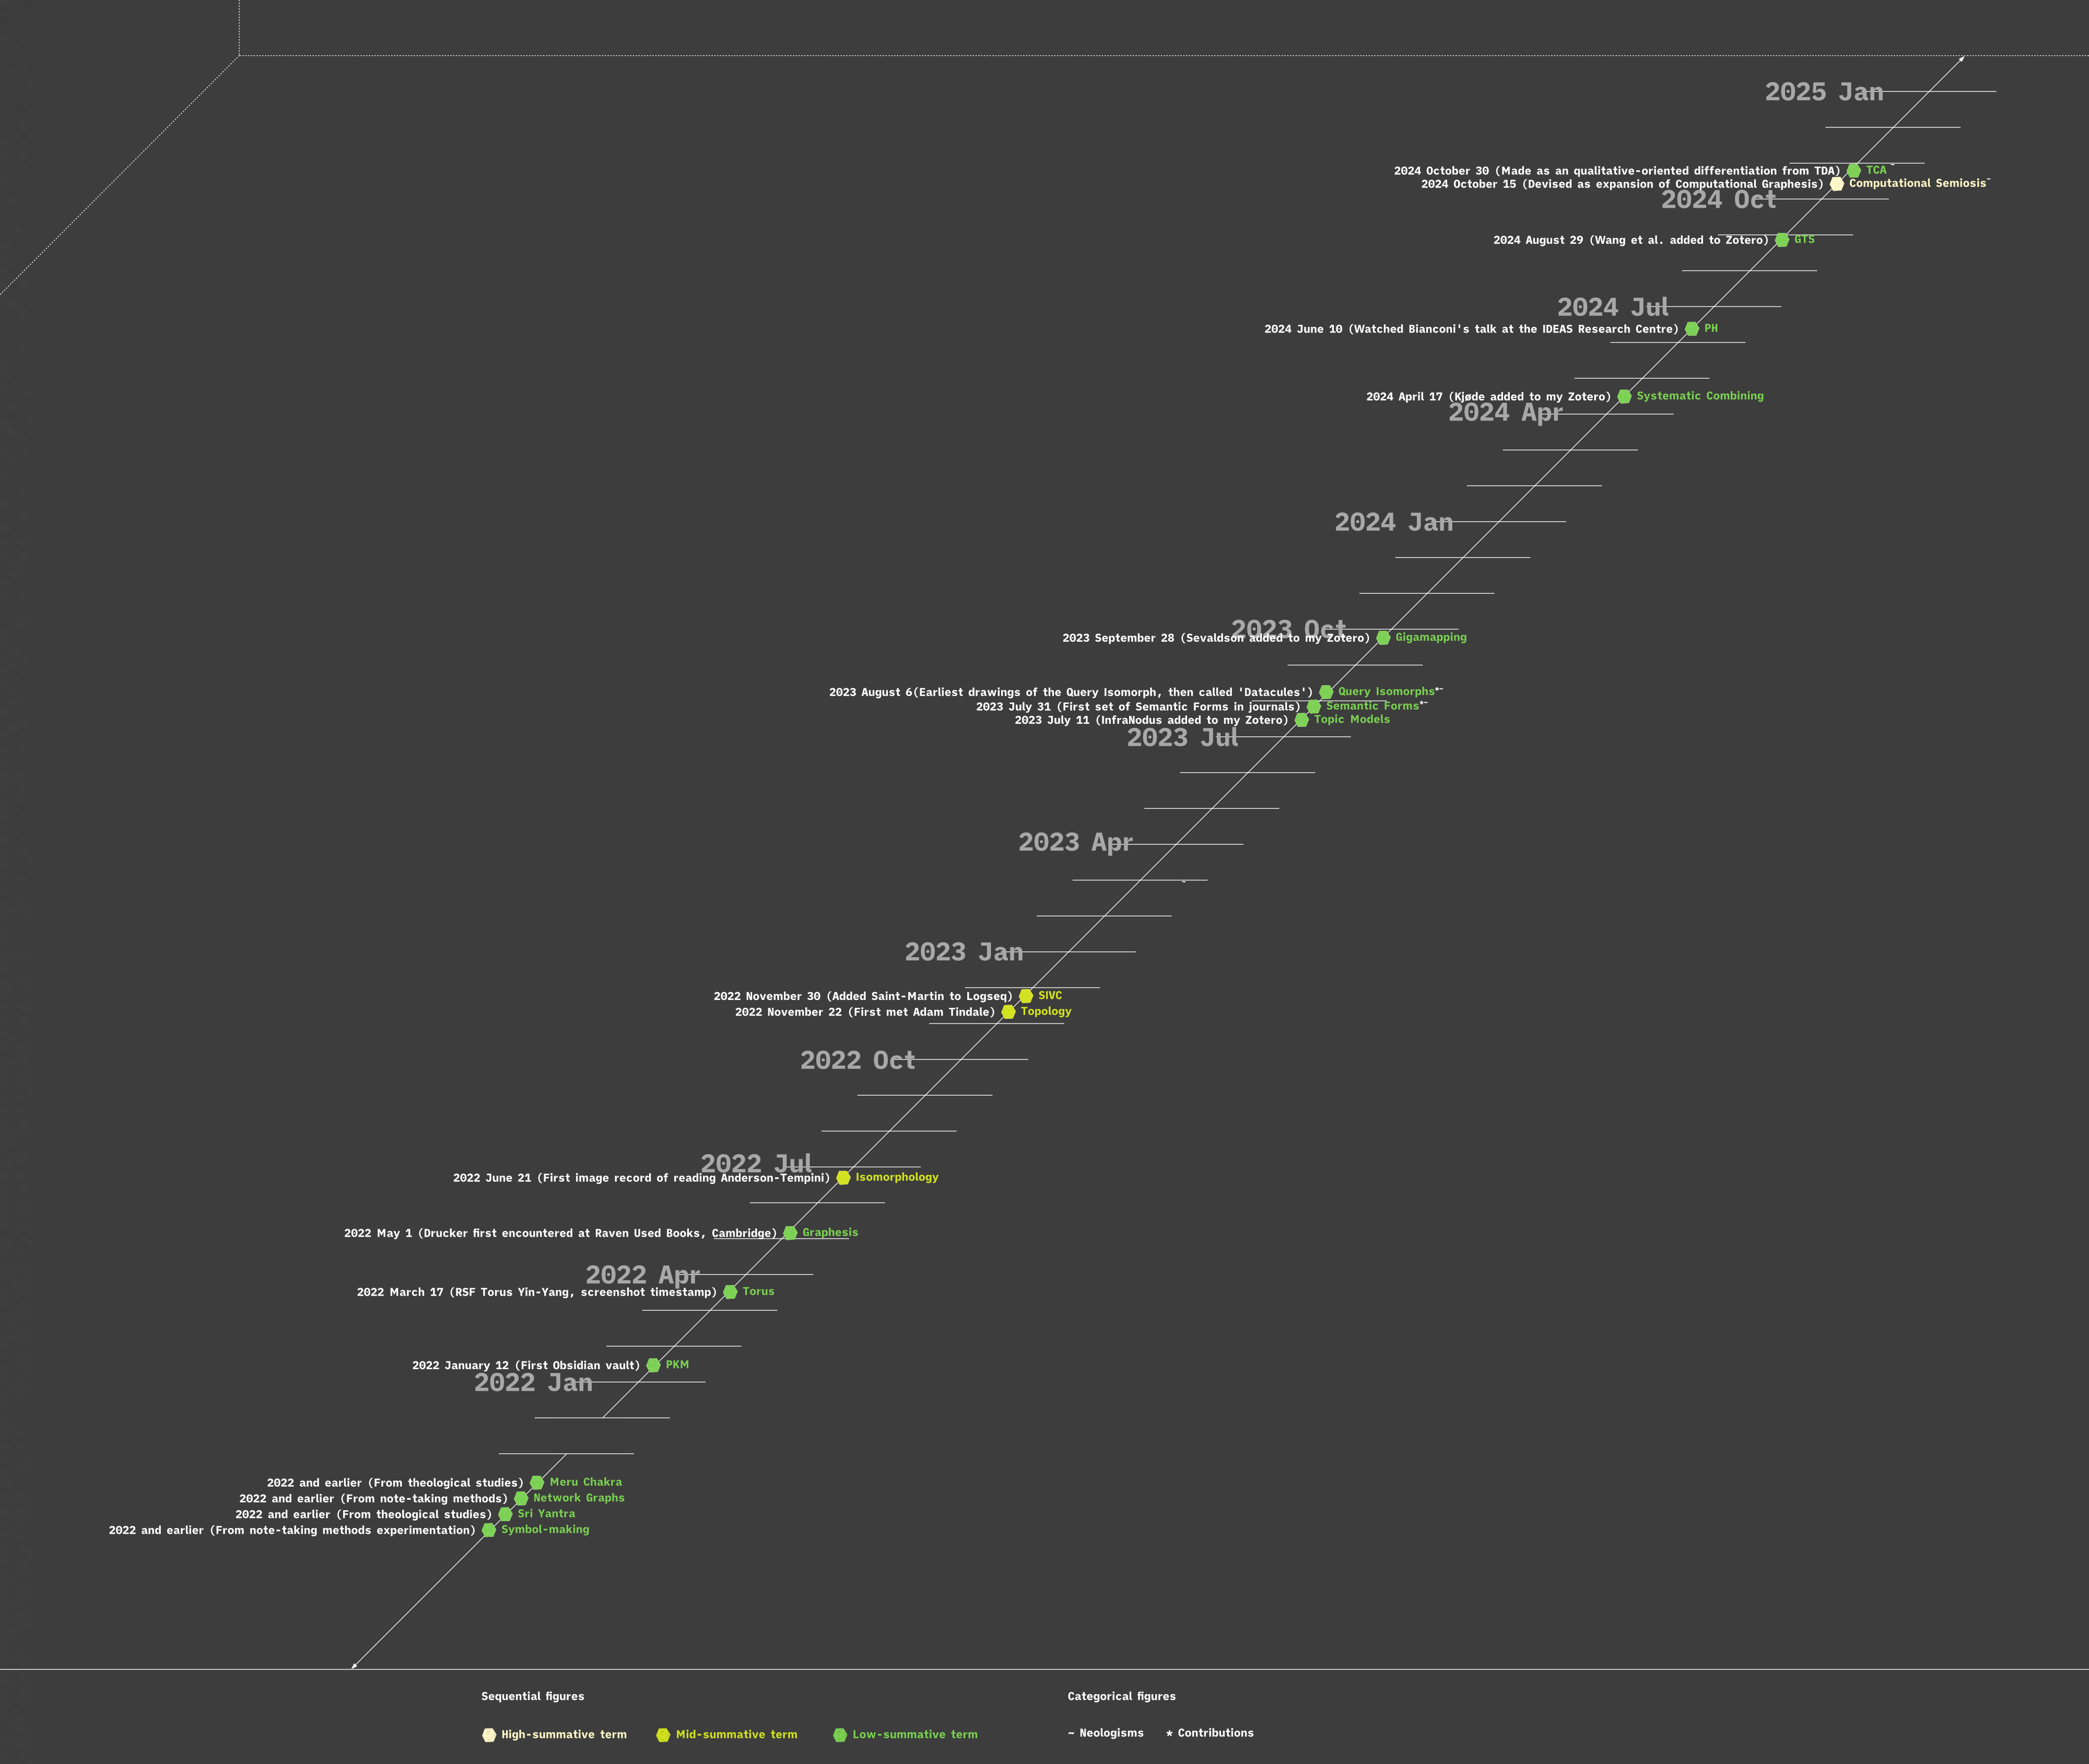
\includegraphics[width=0.7\textwidth]{figures/5.11.Time line.png}
    \caption[Sample \textit{s} ideas on a rectilinear timeline]{\textbf{Sample \textit{s} ideas on a rectilinear timeline.}}
    \label{f5.11.Time line}
\end{figure}

\begin{figure}[h!]
    \centering
    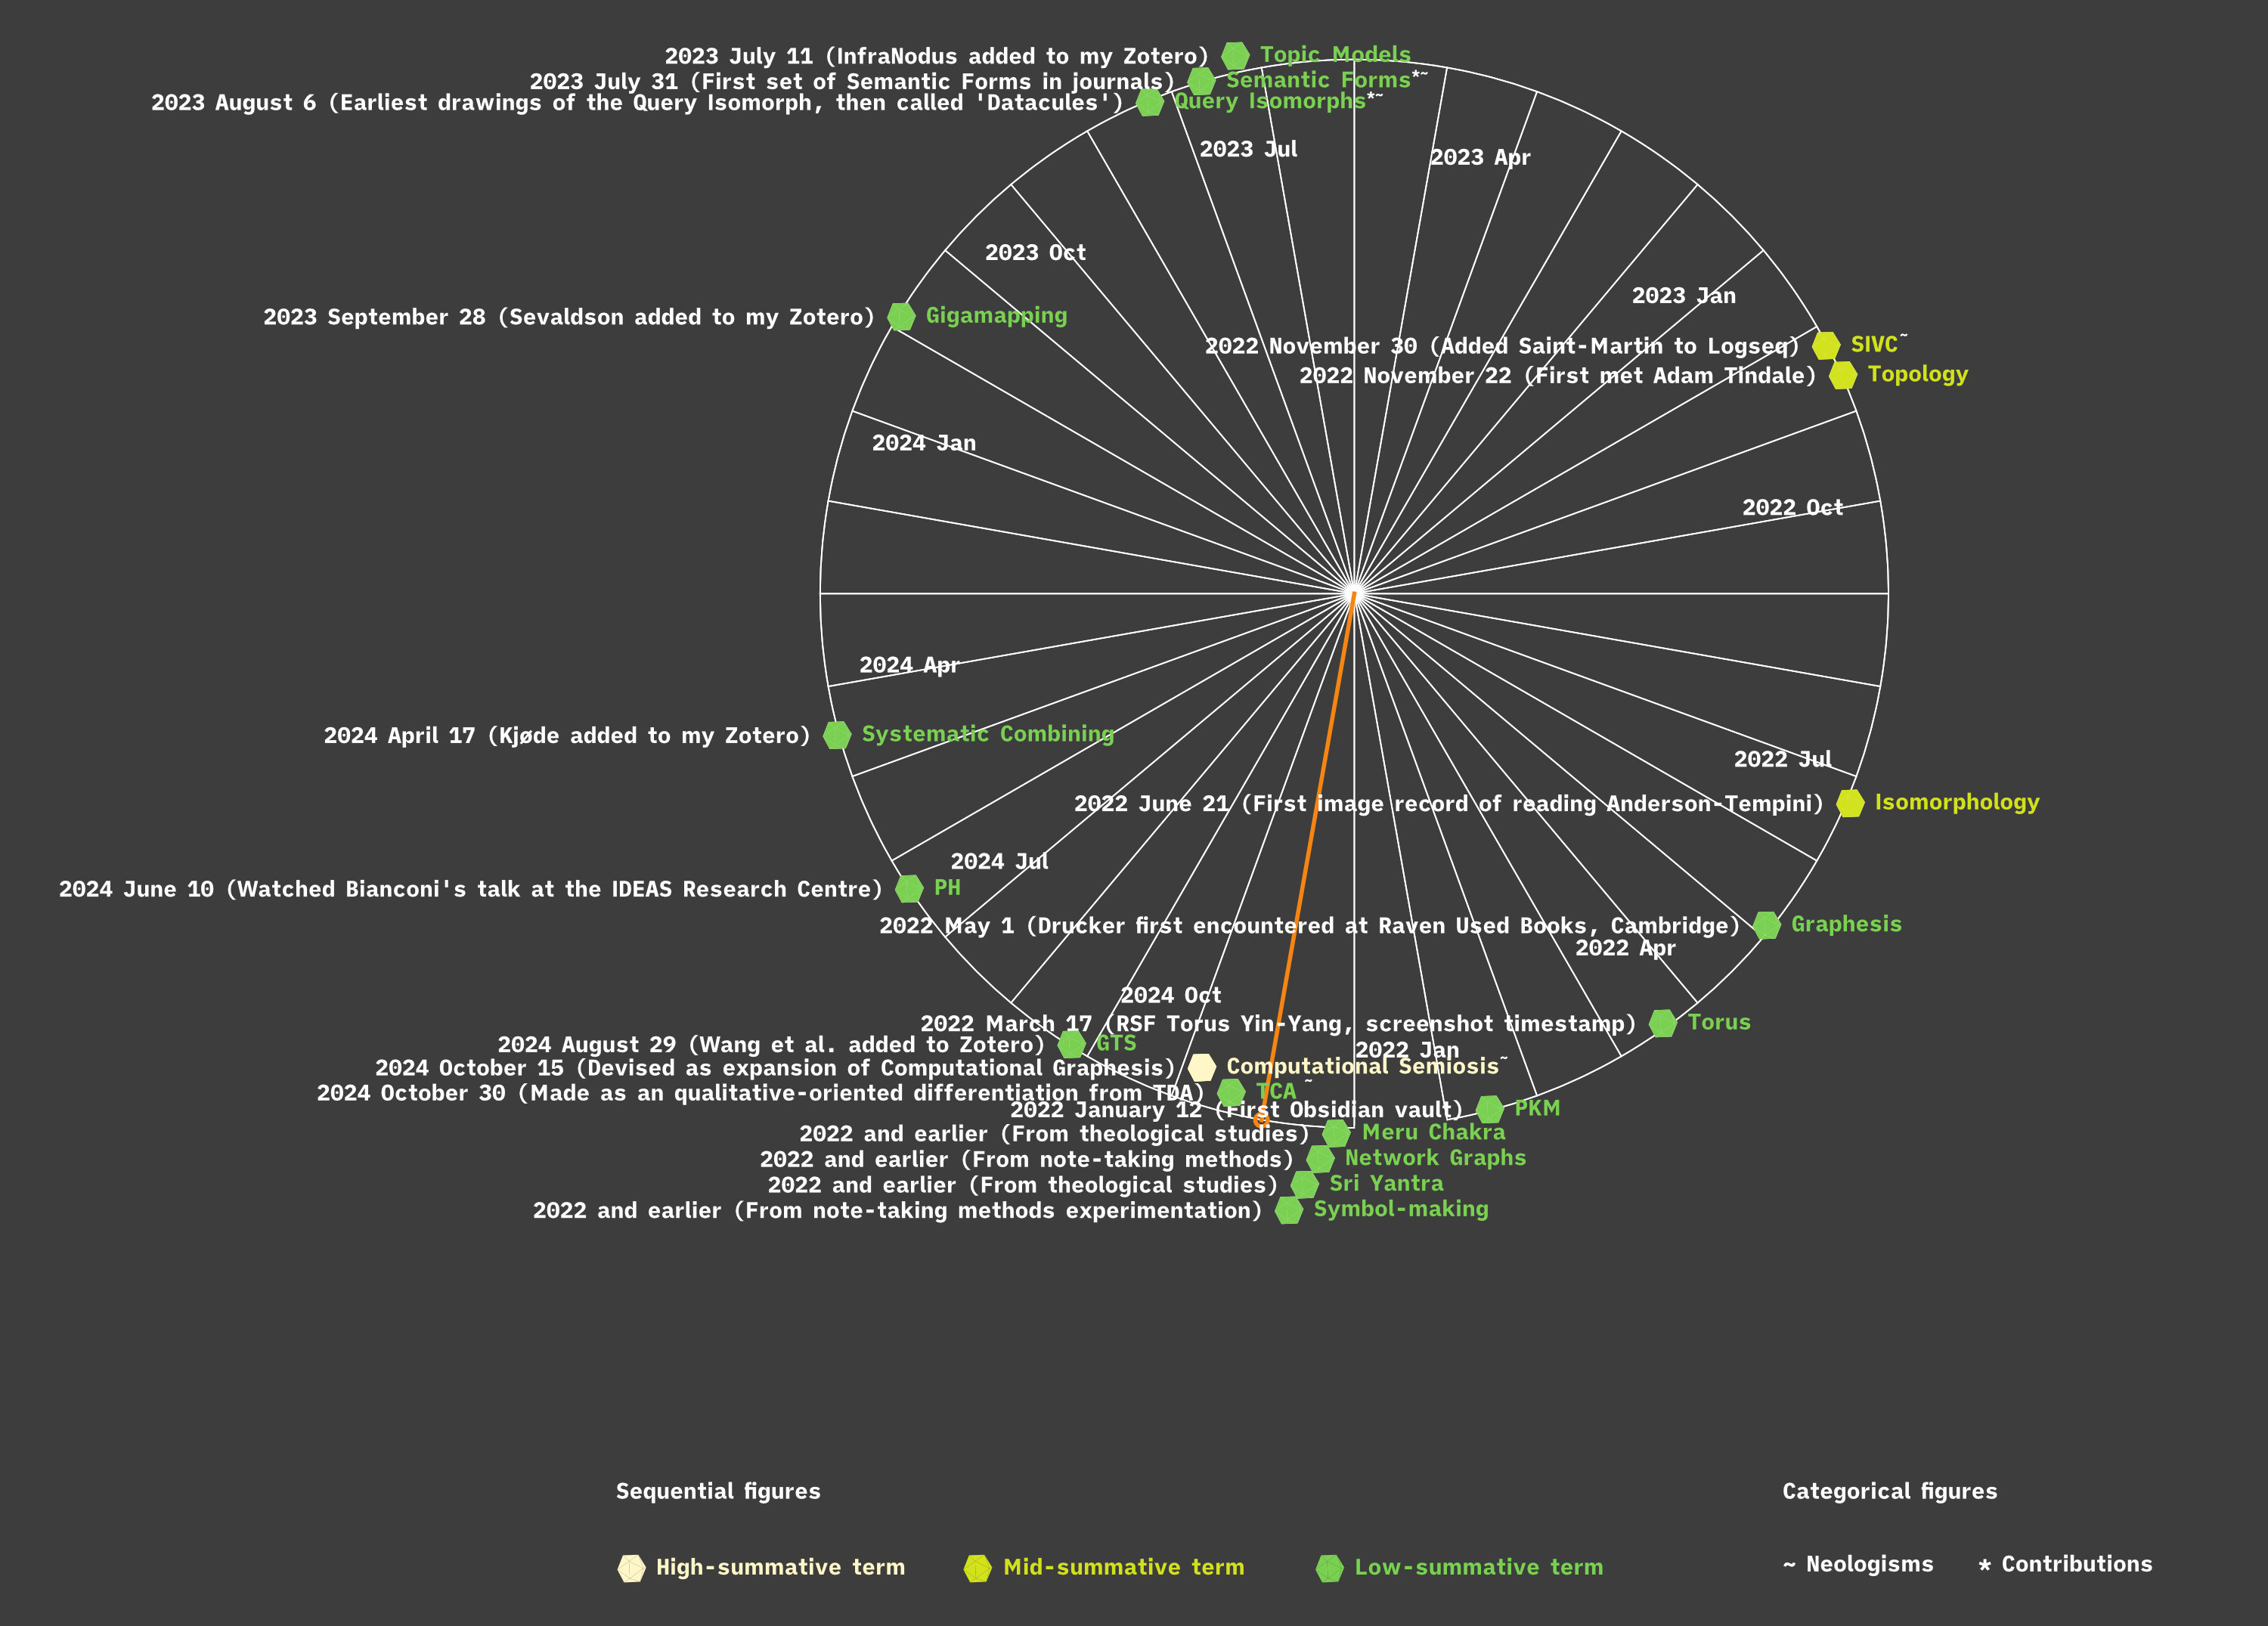
\includegraphics[width=0.7\textwidth]{figures/5.11.Time circle.png}
    \caption[Sample \textit{s} ideas on an elliptical cycle timeline]{\textbf{Sample \textit{s} ideas on an elliptical cycle timeline.}}
    \label{f5.11.Time circle}
\end{figure}
\FloatBarrier  



\subsection{Experiments in Visuospatialization: Query Isomorph \textit{i} in Semantic Forms}
\subsubsection{Introducing Query Isomorph \textit{i}}

\textbf{\textit{i} as a name}
\\

The name `i' may seem to point to the popular prefix used to signify individual customizability of many iProducts, but it was named primarily for other reasons. The scholastic practice of incipit identified works by their first few opening words \citep[p. 3]{smith_book_2001} \footnote{For a thorough introduction of the incipit, its medieval use, and its ideological significance, see the introduction of \textit{Book of the Incipit : Beginnings in the Fourteenth Century} \citep[p. 3]{smith_book_2001}}. Query Isomorph `i', then is named after the first letter of the word `Isomorph'. Second, as play on scale using miniature symbolic representation, the letter `i' seems to depict a small person with a body and a head, whimsically calling attention to the ways text-and ideas- are a space that we move through; third, and by extension, the `i' is autobiographical in that, like any work, this thesis is in a sense a self-portrait of its maker. Fourth, the letter `i' uses one point and one line, the first and first-dimensional building blocks of all network graphs in all dimensions. To articulate this point further in topological terms, because I propose the Query Isomorph as a tool in Topological Capta Analysis, the point of the 'i' represents the 0-dimensional simplex, or the point, and the bar of the 'i' represents the 1-dimensional simplex, or the line segment \citep[p. 3]{maletic_statistical_2011}.
\index[terms]{incipit} \index[terms]{simplex} \index[terms]{network graph} \index[terms]{symbolic representation} \index[terms]{Topological Capta Analysis} \index[terms]{Topological Capta Analysis (TCA)} \index[terms]{Query Isomorph} 



\textbf{Two-dimensional and three-dimensional Query Isomorph configurations}
\\

\FloatBarrier  
\begin{figure}[h]
    \centering
    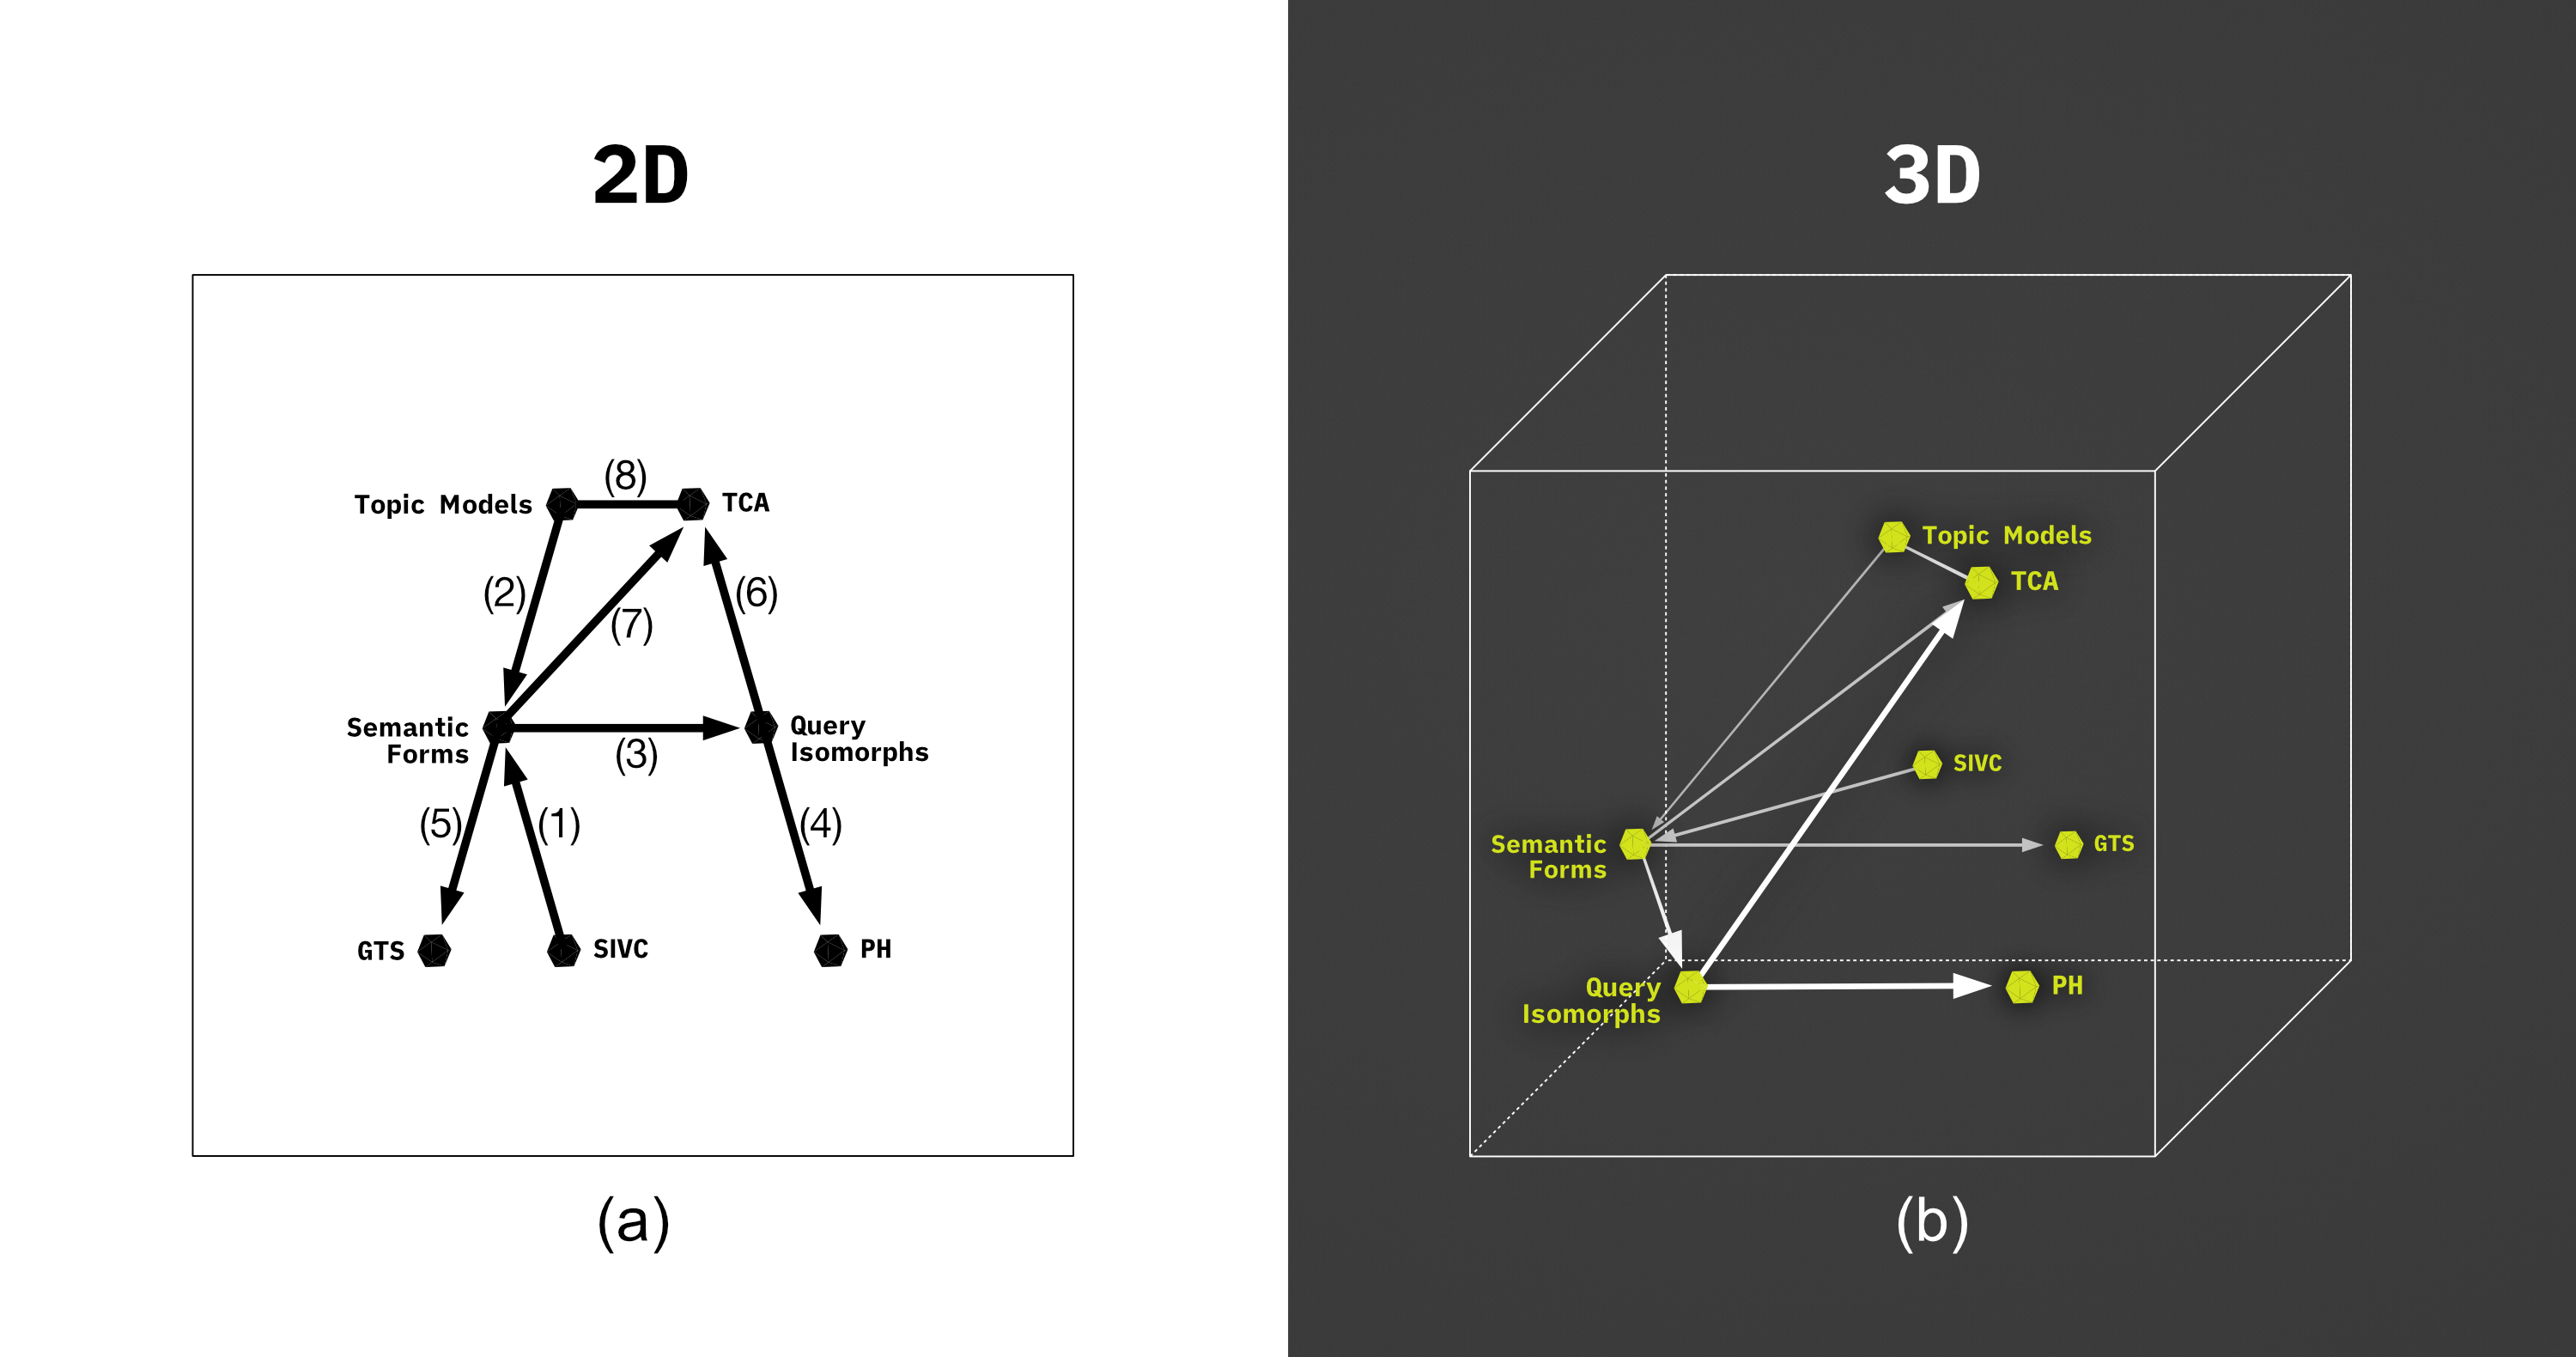
\includegraphics[width=0.8\textwidth]{figures/5.7.Q i.png}
    \caption[Query Isomorph \textit{i} in 2D and 3D]{\textbf{Query Isomorph \textit{i} in 2D and 3D.}
}
    \label{f5.7.Q i}
\end{figure}
\index[terms]{TCA Workspace}
\index[people]{Sowa, John F.}
\clearpage
\FloatBarrier


\autoref{f5.7.Q i} is a depiction of how a researcher might query this thesis using Query Isomorph \textit{i} in two-dimensional and three-dimensional directed graphlet formats. \autoref{f5.7.Q i} (a) has eight numbered Query Isomorph graph edges; 1-5 are directed edges which align with the order of ideas in Sample \textit{s}; Note that 4, 5, and 6 indicate that Query Isomorphs lead me to Persistence Homology (PH), which facilitates 5 as a connection from Semantic Forms to Global Topological Synchronization (GTS)- both 4 and 5 are required to move to TCA, which I arrive to through Query Isomorphs first in 6 because I arrive to the topological ideas of PH via Query Isomorphs, and not through Semantic Forms in 7; 8 represents is an example of an undirected Query Isomorph edge in use, meaning the fictional researcher using Query Isomorph \textit{i} is not looking for a particular derivation sequence between these two ideas, Topic Models and TCA in this case. \autoref{f5.7} 

(b) depicts the same Query Isomorph in (a) with the addition of spatial placement via 3D interface. In this case verticality is used as a method to encode hierarchy into the query. For example, in (b), by placing it higher, the fictional researcher here is querying for how TCA acts as a category for Semantic Forms and Query Isomorphs. The depth of the visuospatial input view affords more space for additional cues for hierarchy and sequence through node placement. 

Many people do not read from left-to-right, so if I were to code this 3D input method I would make sure to adapt the interface for the TCA Workspace user. For example, a feature that automatically populates directed Query Isomorph edges between nodes depending on their placement along the horizontal axis would adapt to the person’s settings of derivation starting from the left or from the right. To be clear, however, the Query Isomorph edge direction would be customizable and not dependent on the node’s position along a horizontal axis only, as I expect will be required for many different query configurations.

\index[terms]{Query Isomorph} \index[terms]{Semantic Forms} \index[terms]{Topological Capta Analysis (TCA)} \index[terms]{Global Topological Synchronization (GTS)}

I conjecture that the benefits of inputting a query of this level of specificity with a directed query graphlet like the Query Isomorph \textit{i}, instead of the above natural language query equivalent, can save some time. In my experience queries are often iterated upon to fine-tune desired information, and altered when insightful correlations are encountered. It is in this sense that the dimensionally versatile Query Isomorph, as input methods shown in \autoref{f5.7.Q i} (a) and (b), represent value by facilitating query iterations through the semiotic affordances of node position and edge direction.
\index[terms]{Query Isomorphs}





\noindent \textbf{The option to represent Semantic Shapes in three-dimensional space}
\\
\FloatBarrier  
\begin{figure}[h!]
    \centering
    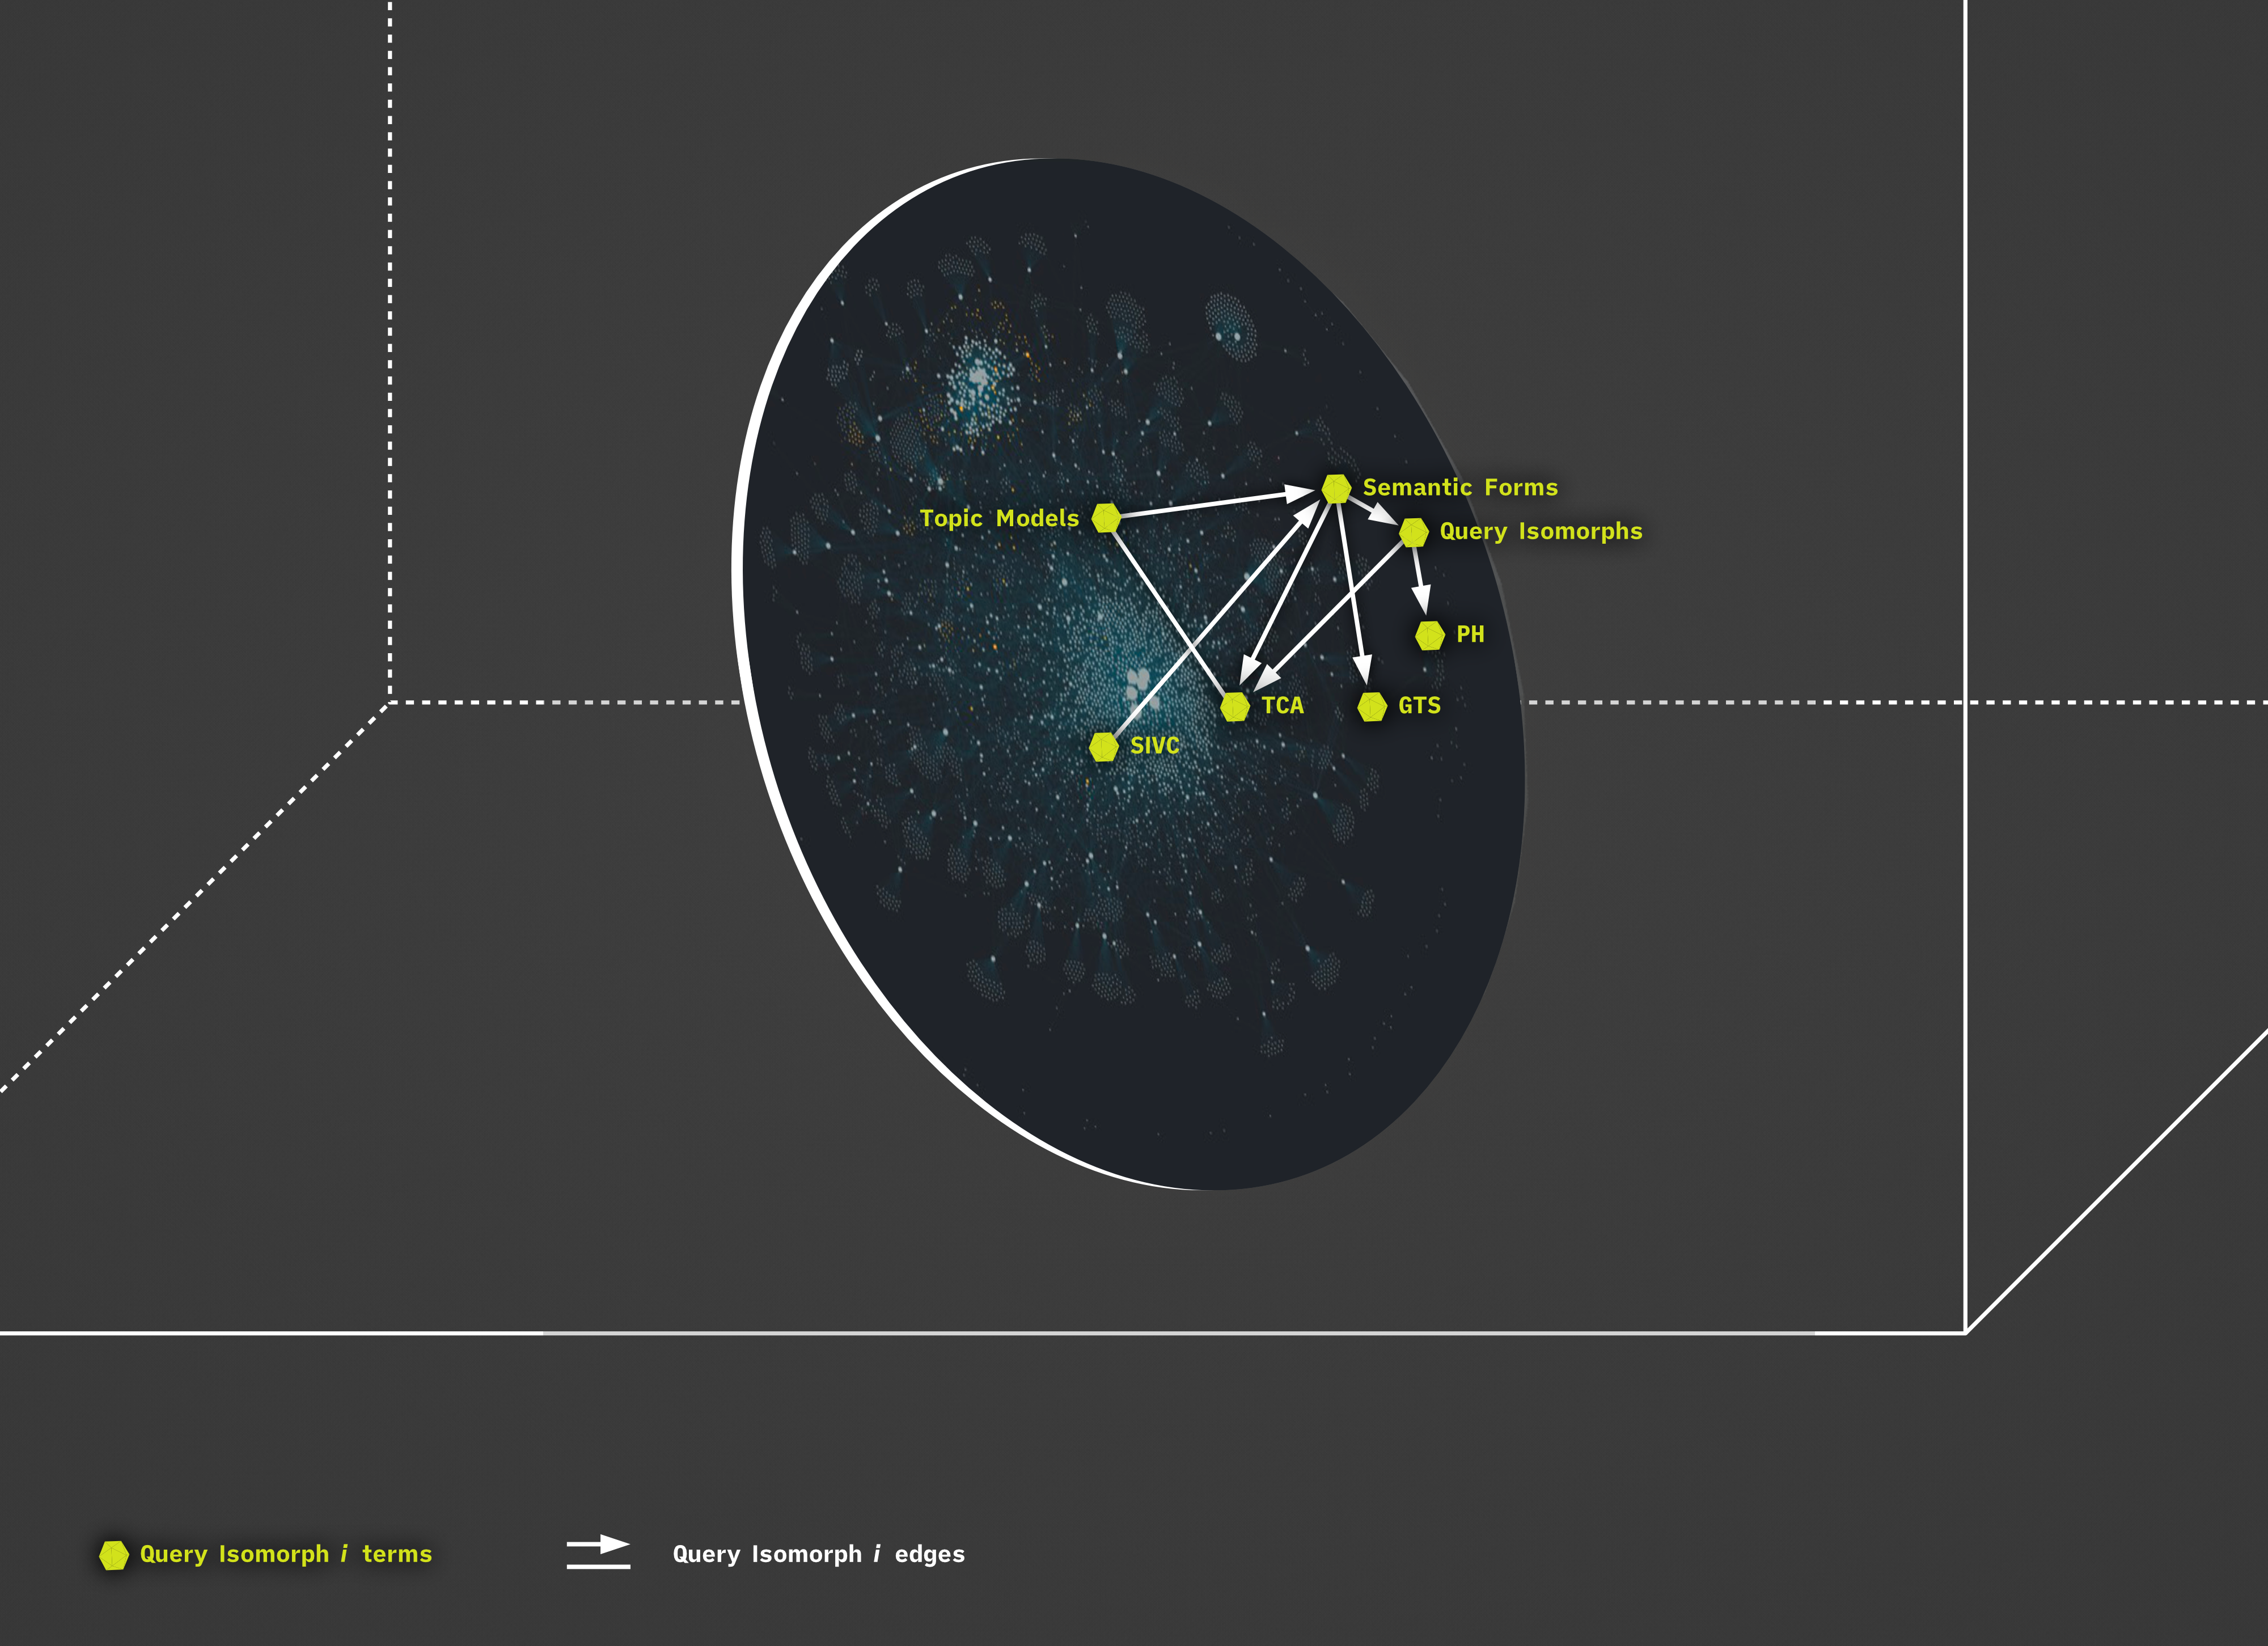
\includegraphics[width=\textwidth]{figures/5.9.Semantic Shape Circle.png}
    \caption[Query Isomorph \textit{i} on a Circle Semantic Shape Logseq network graph]{\textbf{Query Isomorph \textit{i} on a Circle Semantic Shape Logseq network graph.}}
    \label{f5.9.Semantic Shape Circle}
\end{figure}
\index[people]{Sowa, John F.}
\par
\FloatBarrier  

I propose that representing the flat Semantic Shapes in three-dimensional space will be valuable. For example, one occasion I expect will be valuable will be the placement of Query Isomorphs in their 3D input configuration alongside the larger graph which they are pulled from. Since I propose TCA Workspace extend the capabilities of PKM platforms, I illustrate here an example of Query Isomorph \textit{i} superimposed onto my Logseq graph. Furthermore, I expect the dimensional versatility of TCA Workspace to include many more applications of models that use both 2D and 3D information visuospatializations. 


\subsubsection{Query Isomorph \textit{i} in six Semantic Forms}
To begin this series of experiments in Computational Semiosis and information visuospatialization, I will illustrate Query Isomorph \textit{i} as it would appear in coded TCA Workspace if it were coded. 

By representing Query Isomorph \textit{i} in the following six Semantic Forms I illustrate the ways the Query Isomorph would be rearranged and warped when placed within the ‘magnetic’ field of each Semantic Form’s semantic force. I made Sample \textit{s}is about this thesis to make it easier for the reader to understand how Query Isomorphs and Semantic Forms could be applied to a text by starting from the text we are already discussing. 

Each of the following illustrations of Query Isomorph \textit{i} in a Semantic Form was rendered by overlaying node-label pairings onto screenshots of my Blender Semantic Form models.

As a continuation of \autoref{f5.3} and \autoref{f5.4} I will present my Semantic Forms as pairings. Each coupling includes a simpler Semantic Form followed by one that is more complex. The Semantic Form pairings that follow are: Cylinder with Ring Torus, Cone with Double Cone, and Sphere with Horn Torus. 
\index[terms]{Ring Torus Semantic Form}
\index[terms]{Sphere Semantic Form}
\index[terms]{Cylinder Semantic Form}
\index[terms]{Horn Torus Semantic Form}
\index[terms]{Cone Semantic Form}
\index[terms]{Double Cone Semantic Form}

\noindent \textbf{Cylinder and Ring Torus}
\\

\textbf{Query Isomorph \textit{i} in the Cylinder and Ring Torus Semantic Forms}
\\

\textbf{\textit{Cylinder Semantic Form}}

\FloatBarrier  
\begin{figure}[h!]
    \centering
    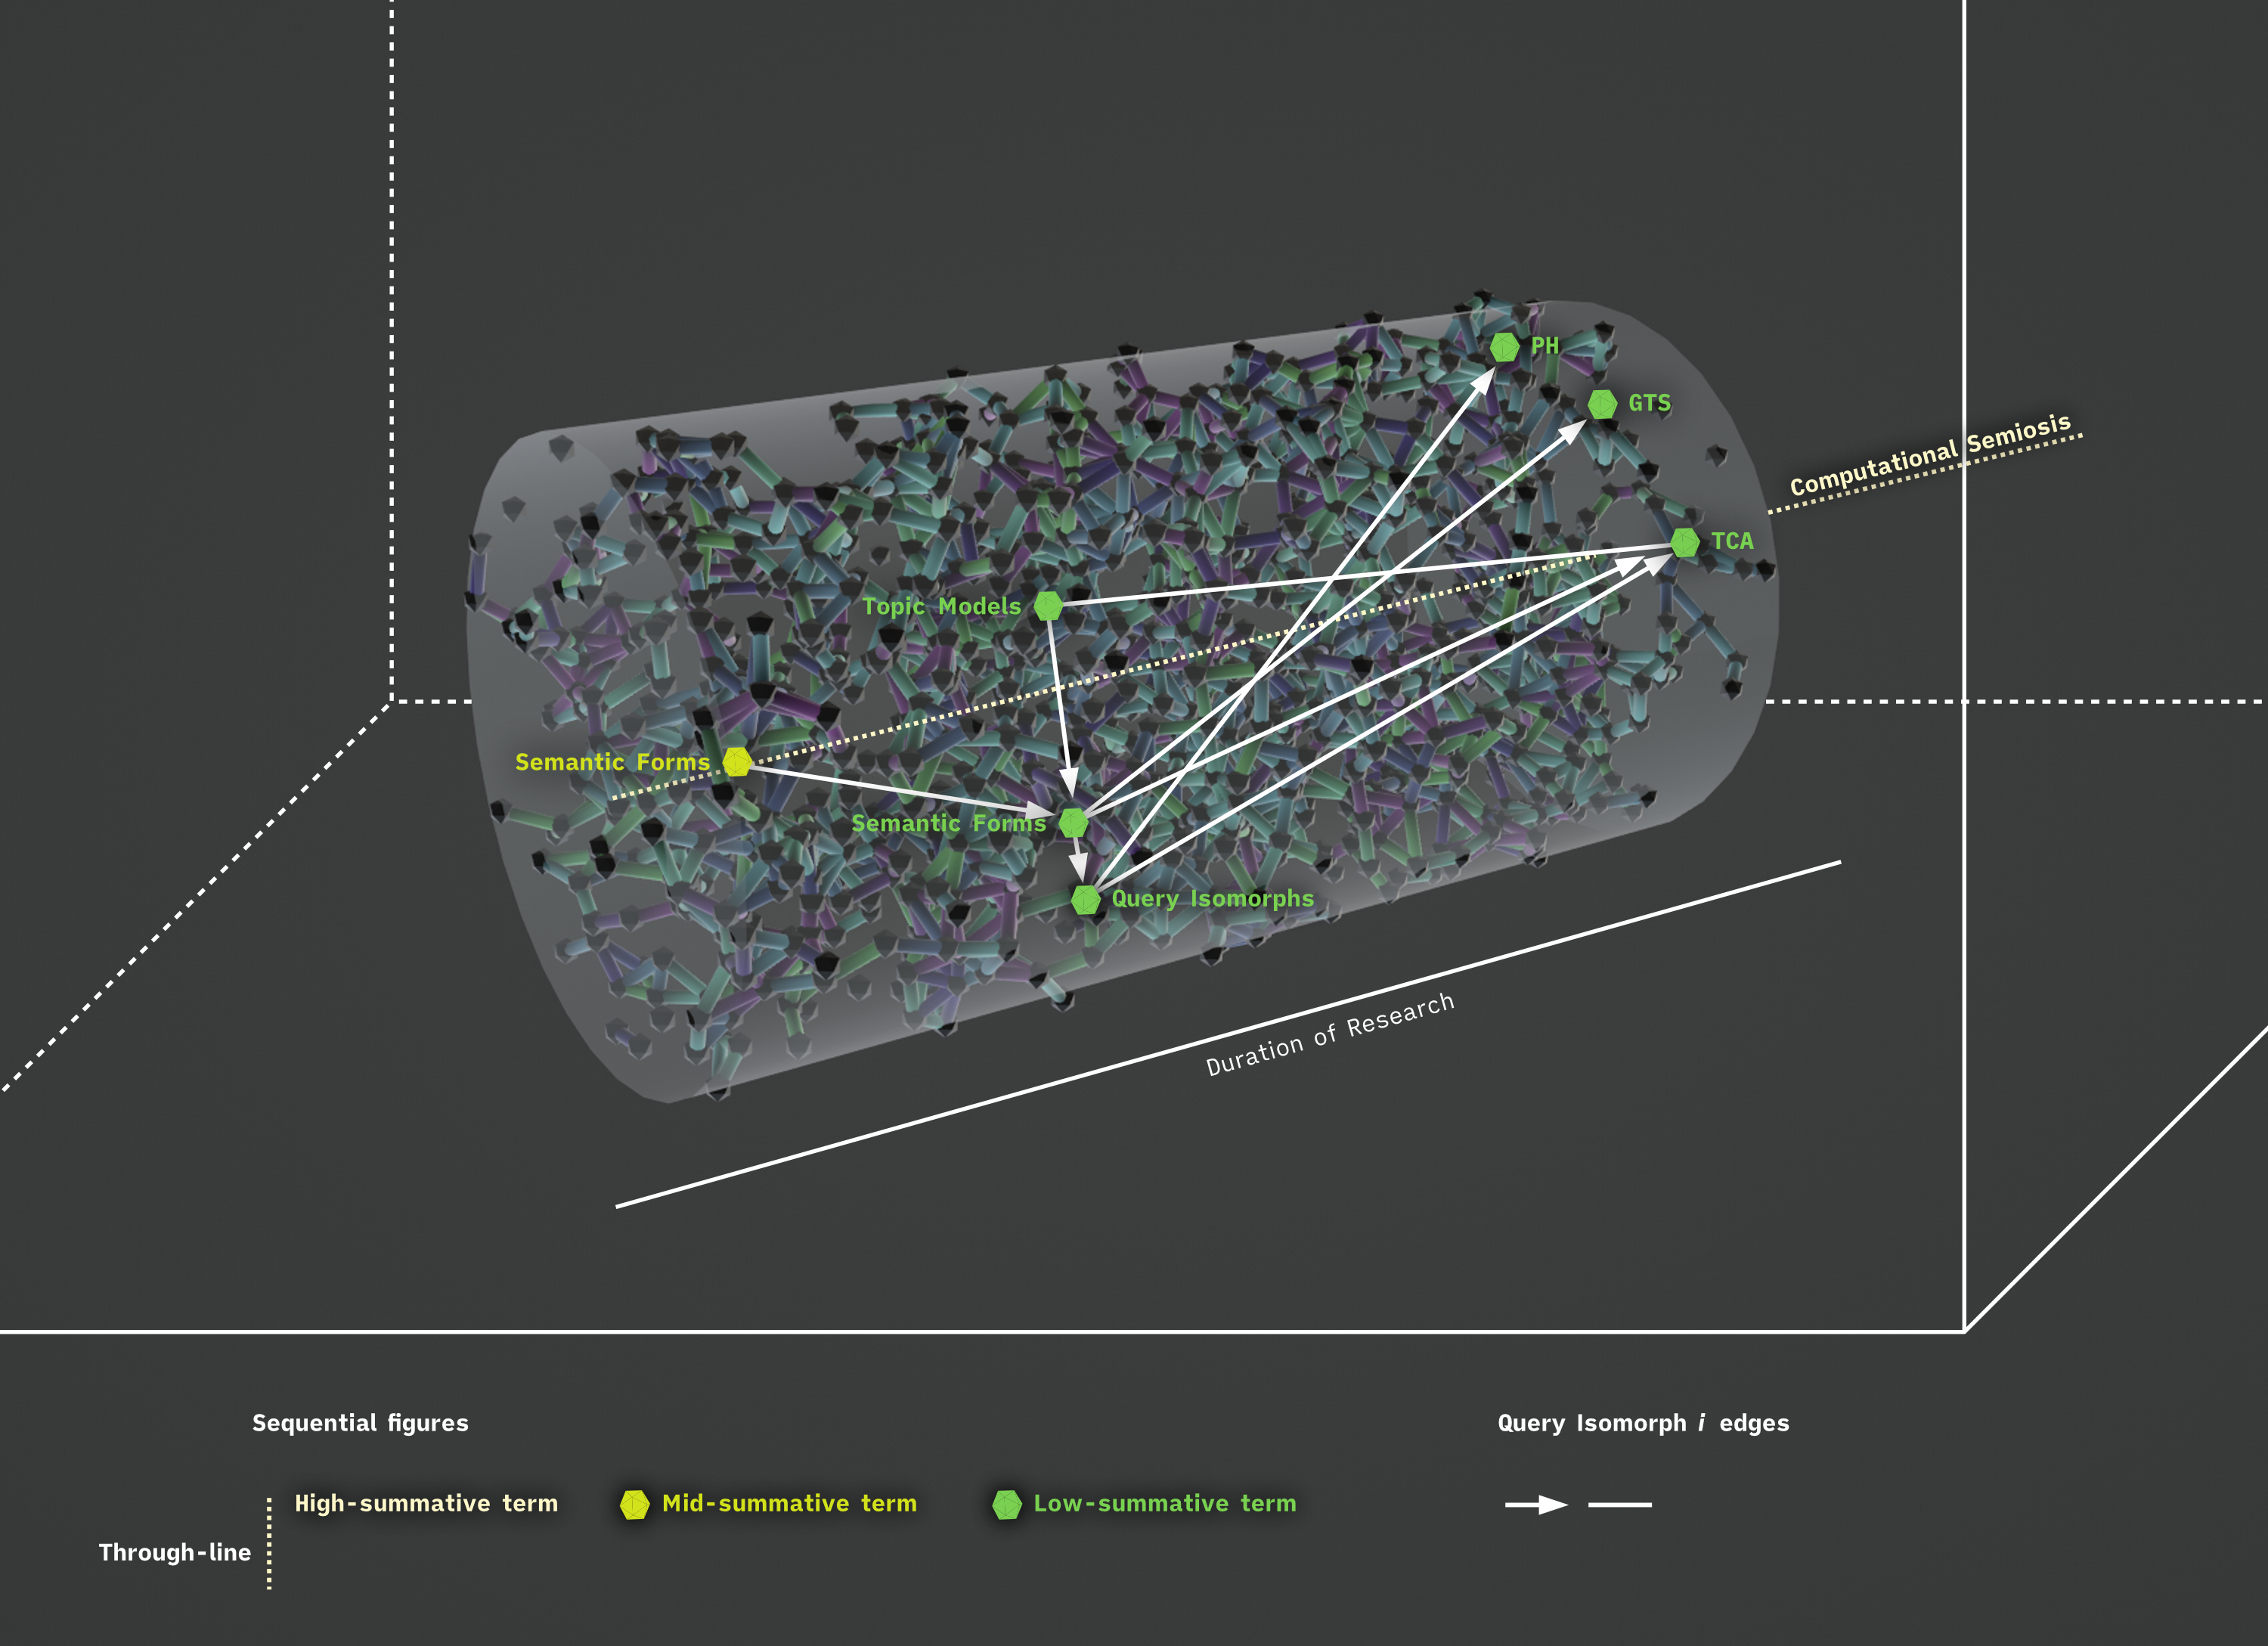
\includegraphics[width=\textwidth]{figures/5.10.Cylinder.png}
    \caption[Cylinder Semantic Form about Query Isomorph \textit{i}]{\textbf{Cylinder Semantic Form about Query Isomorph \textit{i}.} }
    \label{f5.10.Cylinder}
\end{figure}
\index[terms]{Cylinder Semantic Form}
\FloatBarrier  

The \autoref{f5.10.Cylinder} Cylinder Semantic Form represents the duration of my research. To assist placing each idea node accurately along the central axis line that runs through the core of the Cylinder’s barrel, I overlaid the timeline from \autoref{f5.11.Time line} onto the image of the Cylinder Semantic Form. However, also note that nodes closer to the rotational axis line of the cylinder are more general or summative terms. For example, Spatial Information Visualization Composition (SIVC) is a more general idea than Query Isomorphs. Graphs in PKM platforms Obsidian and Logseq tend to place more densely connected terms in the middle of the graph. Since I am representing a series of PKM graphs as the Cylinder Semantic Form, I am adhering to the principle that more densely connected terms, in this case more general terms, are placed toward the middle of the two-dimensional graph. Conversely, less summative terms, like Persistence Homology (PH) are represented as less densely connected, and as such placed closer to the periphery of the Cylinder Semantic Form. 

I propose that one of the through-lines of my thesis document is Computational Semiosis, which is labelled in \autoref{f5.10.Cylinder} as a light yellow dashed line through the middle of the Cylinder barrel. I propose that metaphor of a ``through-line" can be made visuospatial with TCA as a means to add clarity to a topic model. The through-line acts as a semantic analogue in Topological Information Analysis of a TDA Principal Curve which passes through the ``middle" of a data cloud. \citep[p. 1]{kegl_learning_2000}, or mean/average line.
\clearpage



\textbf{Ring Torus Semantic Form}

\FloatBarrier  
\begin{figure}[h!]
    \centering
    \includegraphics[width=\textwidth]{figures/5.12.RT1.png}
    \caption[Ring Torus Semantic Form about Query Isomorph \textit{i}: rectilinear edges]{\textbf{Ring Torus Semantic Form about Query Isomorph \textit{i}: rectilinear edges}}
    \label{f5.12.RT1}
\end{figure}
\index[terms]{Ring Torus Semantic Form}
\FloatBarrier

I visualized the warp of input Query Isomorph \textit{i} in the output Ring Torus Semantic Form in two ways: In \autoref{f5.12.RT1}  I illustrated Query Isomorph edges using rectilinear edges to emphasize the derivation of each Query Isomorph \textit{i} node. In \autoref{f5.12aRT2} I illustrated the Query Isomorph edges using long arcs that aligning with curvature of the Ring Torus. This second style of edges emphasizes the sequence of each Query Isomorph \textit{i} node along the elliptical timeline.I anticipate that toggling between both options will be valuable in the Ring Torus Semantic Form, the Horn Torus Semantic Form, and in any future Semantic Forms that involve curved plotting. 

\autoref{f5.12.RT1} (a) indicates the Loop Seam between the earliest dates and the latest dates along the timeline circle. Dates from Sample \textit{s} that were dated as “2022 and earlier” are labelled in a time segment to the right of the Loop Seam and left of “Jan 2022”. (b) In the case of the Ring Torus Semantic Form, the through-line circles back into itself in what I am calling a Loop-line. The Loop-line represents a theme or themes that are both strongly present in a TCA database within a given time range and are expected to be perpetuated if existing semantic patterns continue. 

A computational method to query for topics that act as through-lines about an Query Isomorph in a Ring Torus Semantic Form would accelerate analysis of texts and text groups. Similar functionality using OpenAI’s GPT-4 to name the relationship between nodes on a graph is already technologically possible, and was shown earlier in a discussion about InfraNodus. To apply the Ring Torus Semantic Form, a researcher querying for through-lines using a ring-torus Semantic Form diagram could use this model to identify which topics in a given text most facilitate the continuation of a given thematic cycle.

To determine accurate node placement within the Ring Torus Semantic Form I overlaid \autoref{f5.11.Time circle} as a guide. Specifically, I warped \autoref{f5.11.Time circle} so that its circumference matched the core line running through the Ring Torus in \autoref{f5.12.RT1}. I then moved each node manually along the radii lines of the superimposed and warped \autoref{f5.11.Time circle} either closer to the inner radius or outer radius of the ring torus depending as my arbitrary measurement of how summative each term is. This technique aligns with the way PKM graphs position nodes in their graphs by placing more highly connected nodes towards the middle as a default. 

\FloatBarrier  
\begin{figure}[h!]
    \centering
    \includegraphics[width=\textwidth]{figures/5.12aRT2.png}
    \caption[Ring Torus Semantic Form about Query Isomorph \textit{i}: curved edges]{\textbf{Ring Torus Semantic Form about Query Isomorph \textit{i}: curved edges}
    \label{f5.12aRT2}}
\end{figure}
\FloatBarrier  


\clearpage

\noindent \textbf{Query Isomorph \textit{i} in the Cone and Double Cone Semantic Forms}
\\
\textbf{\textit{Cone Semantic Form}}
\FloatBarrier  
\begin{figure}[h!]
    \centering
    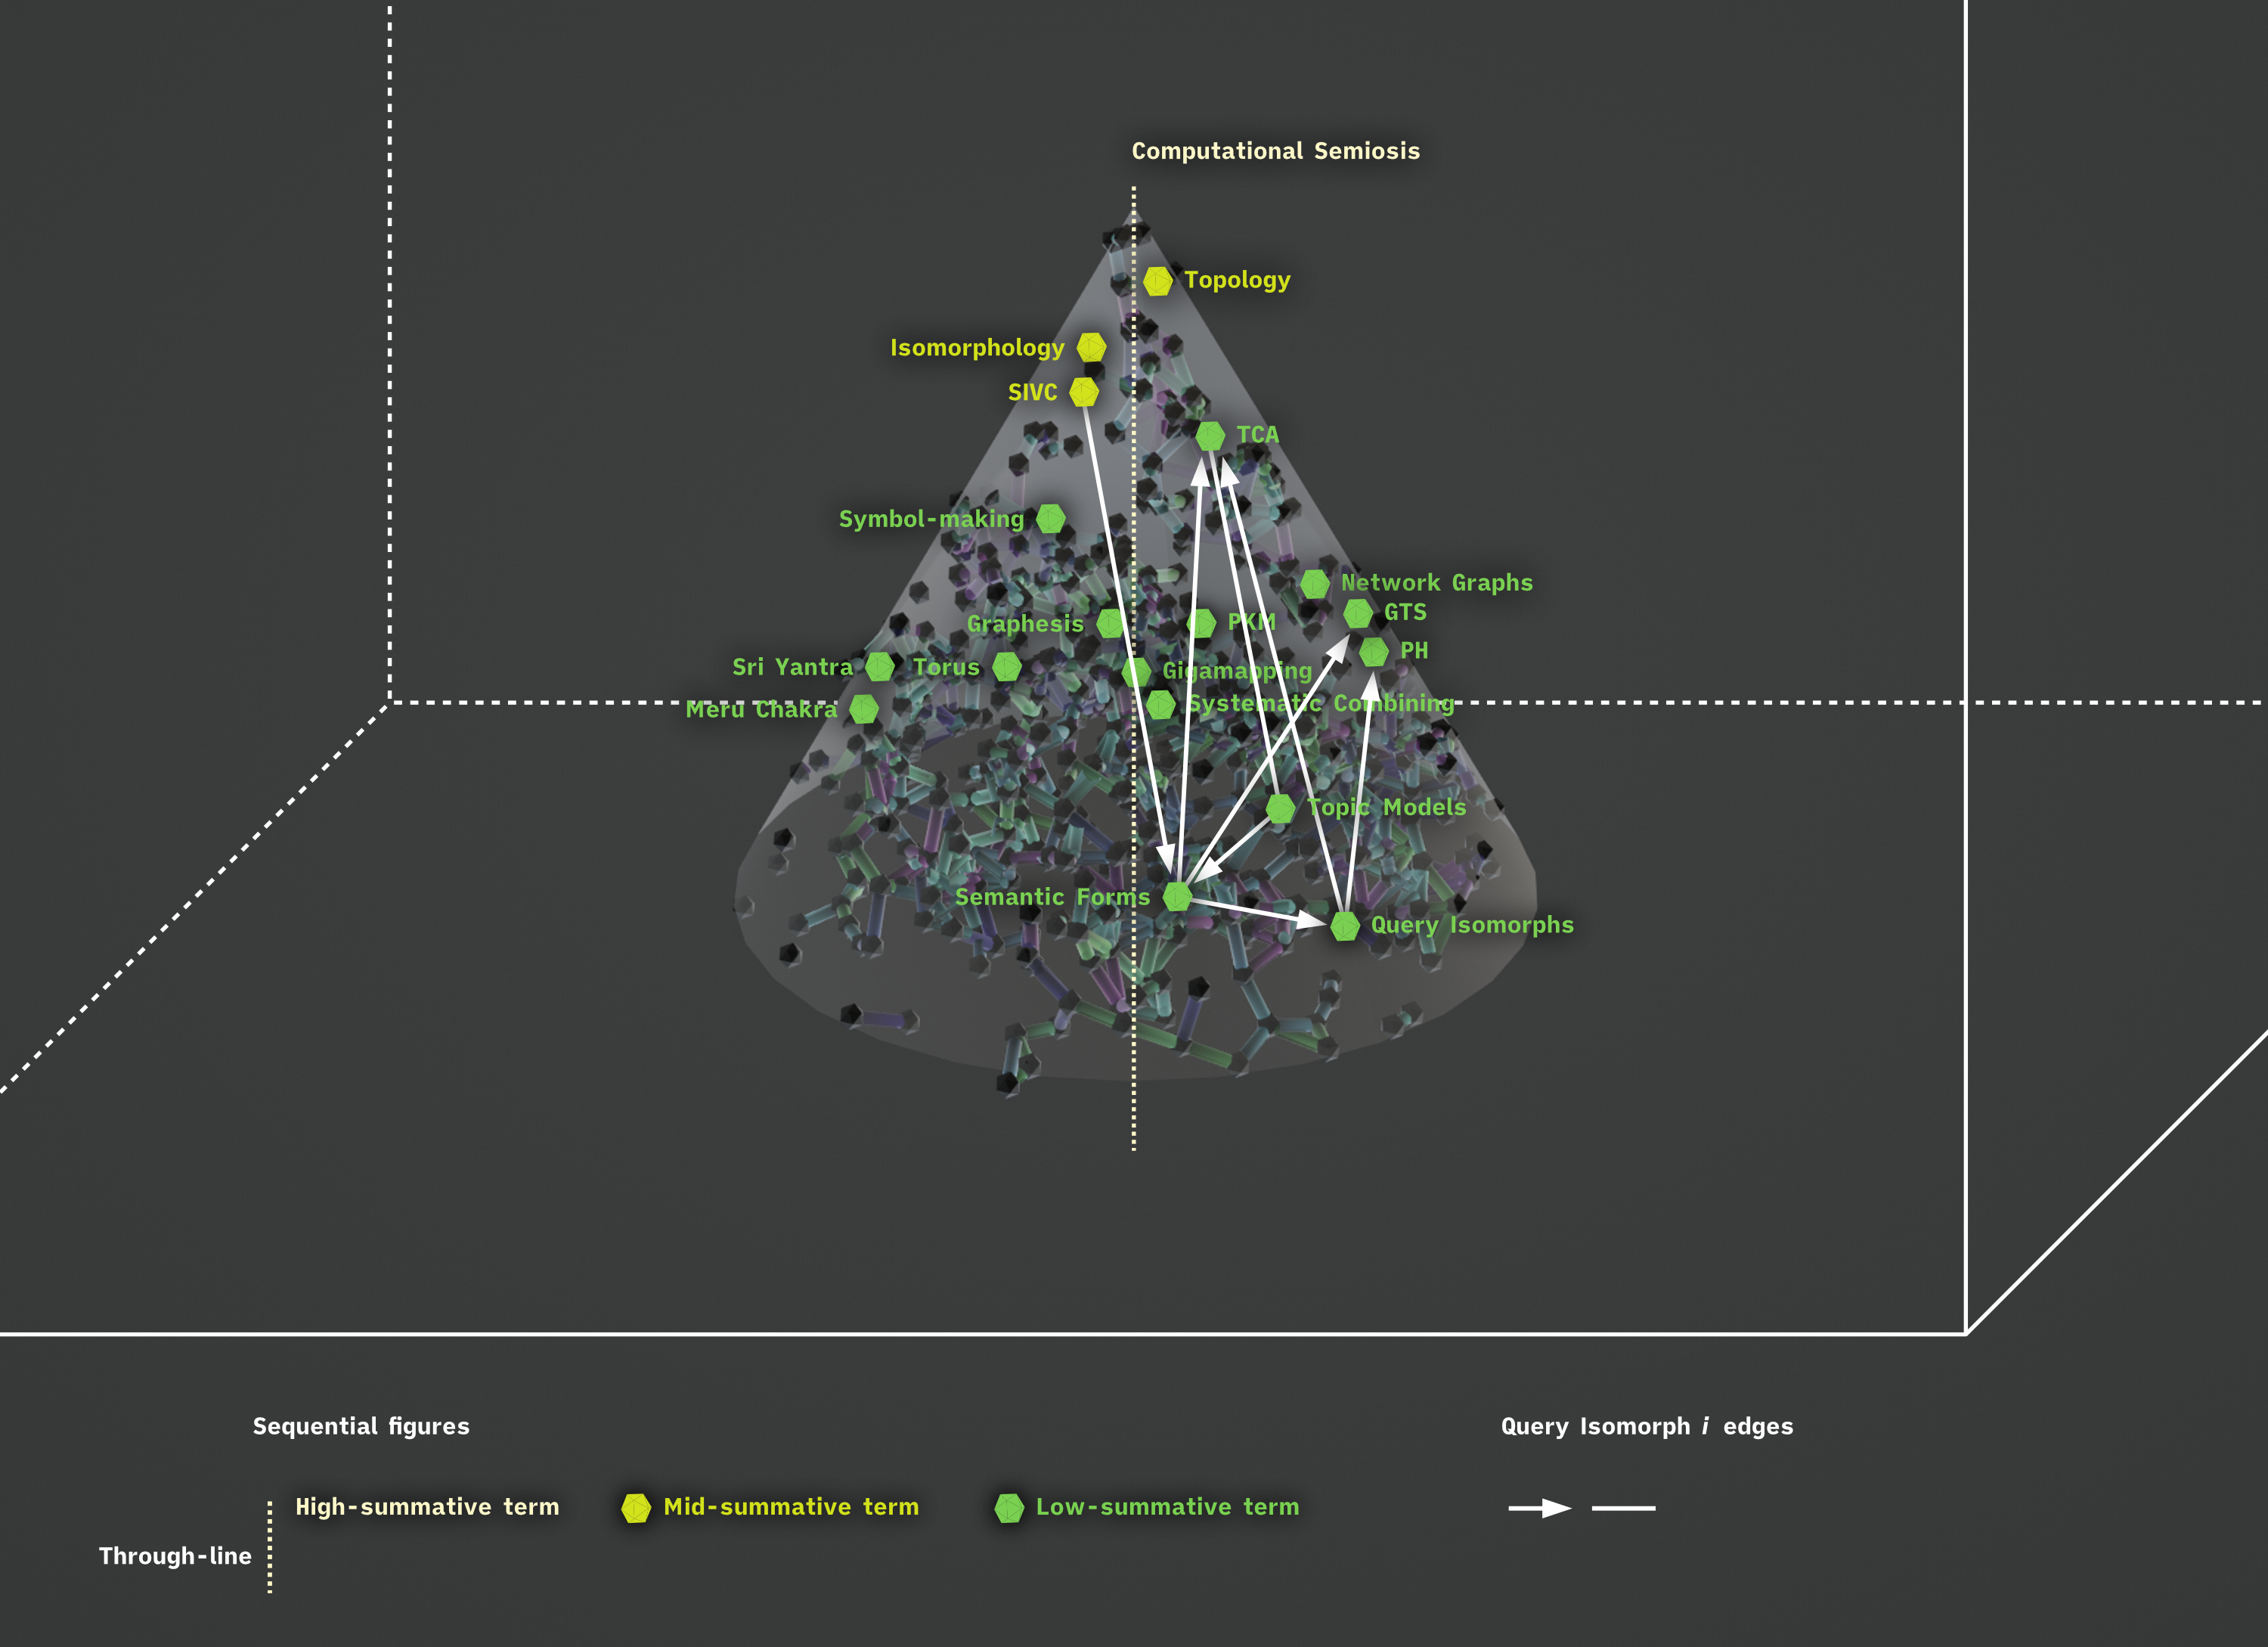
\includegraphics[width=\textwidth]{figures/5.13.Cone.png}
    \caption[Cone Semantic Form about Query Isomorph \textit{i}]{\textbf{Cone Semantic Form about Query Isomorph \textit{i}.}}
    \label{f5.13}
\end{figure}
\FloatBarrier  
The Cone Semantic Form warps input Query Isomorph \textit{i} vertically and horizontally by arranging nodes into a hierarchy of summativeness. This differs from the Cylinder and Ring Torus Semantic Forms because node placement in the Cone Semantic Form does not emphasize when a given concept was added to a TCA database. 

The Cone Semantic Form, then, offers substantial clarity by doubly encoding the highly summative nodes closer to the Cone's peak, followed my mid-summative nodes and low-summative nodes in sequence towards the Cone base. Query Isomorph \textit{i} is labelled by connecting its nodes with white edges. 

The summative arrangement of the Cone Semantic Form works similarly to the with Ontological Semantic Network Summaries in that the terms which are fewer in number towards the top point are the most summative, and have the most subsequent terms derived from them. 

\noindent  \textbf{Double Cone Semantic Form}
\FloatBarrier  
\begin{figure}[h!]
    \centering
    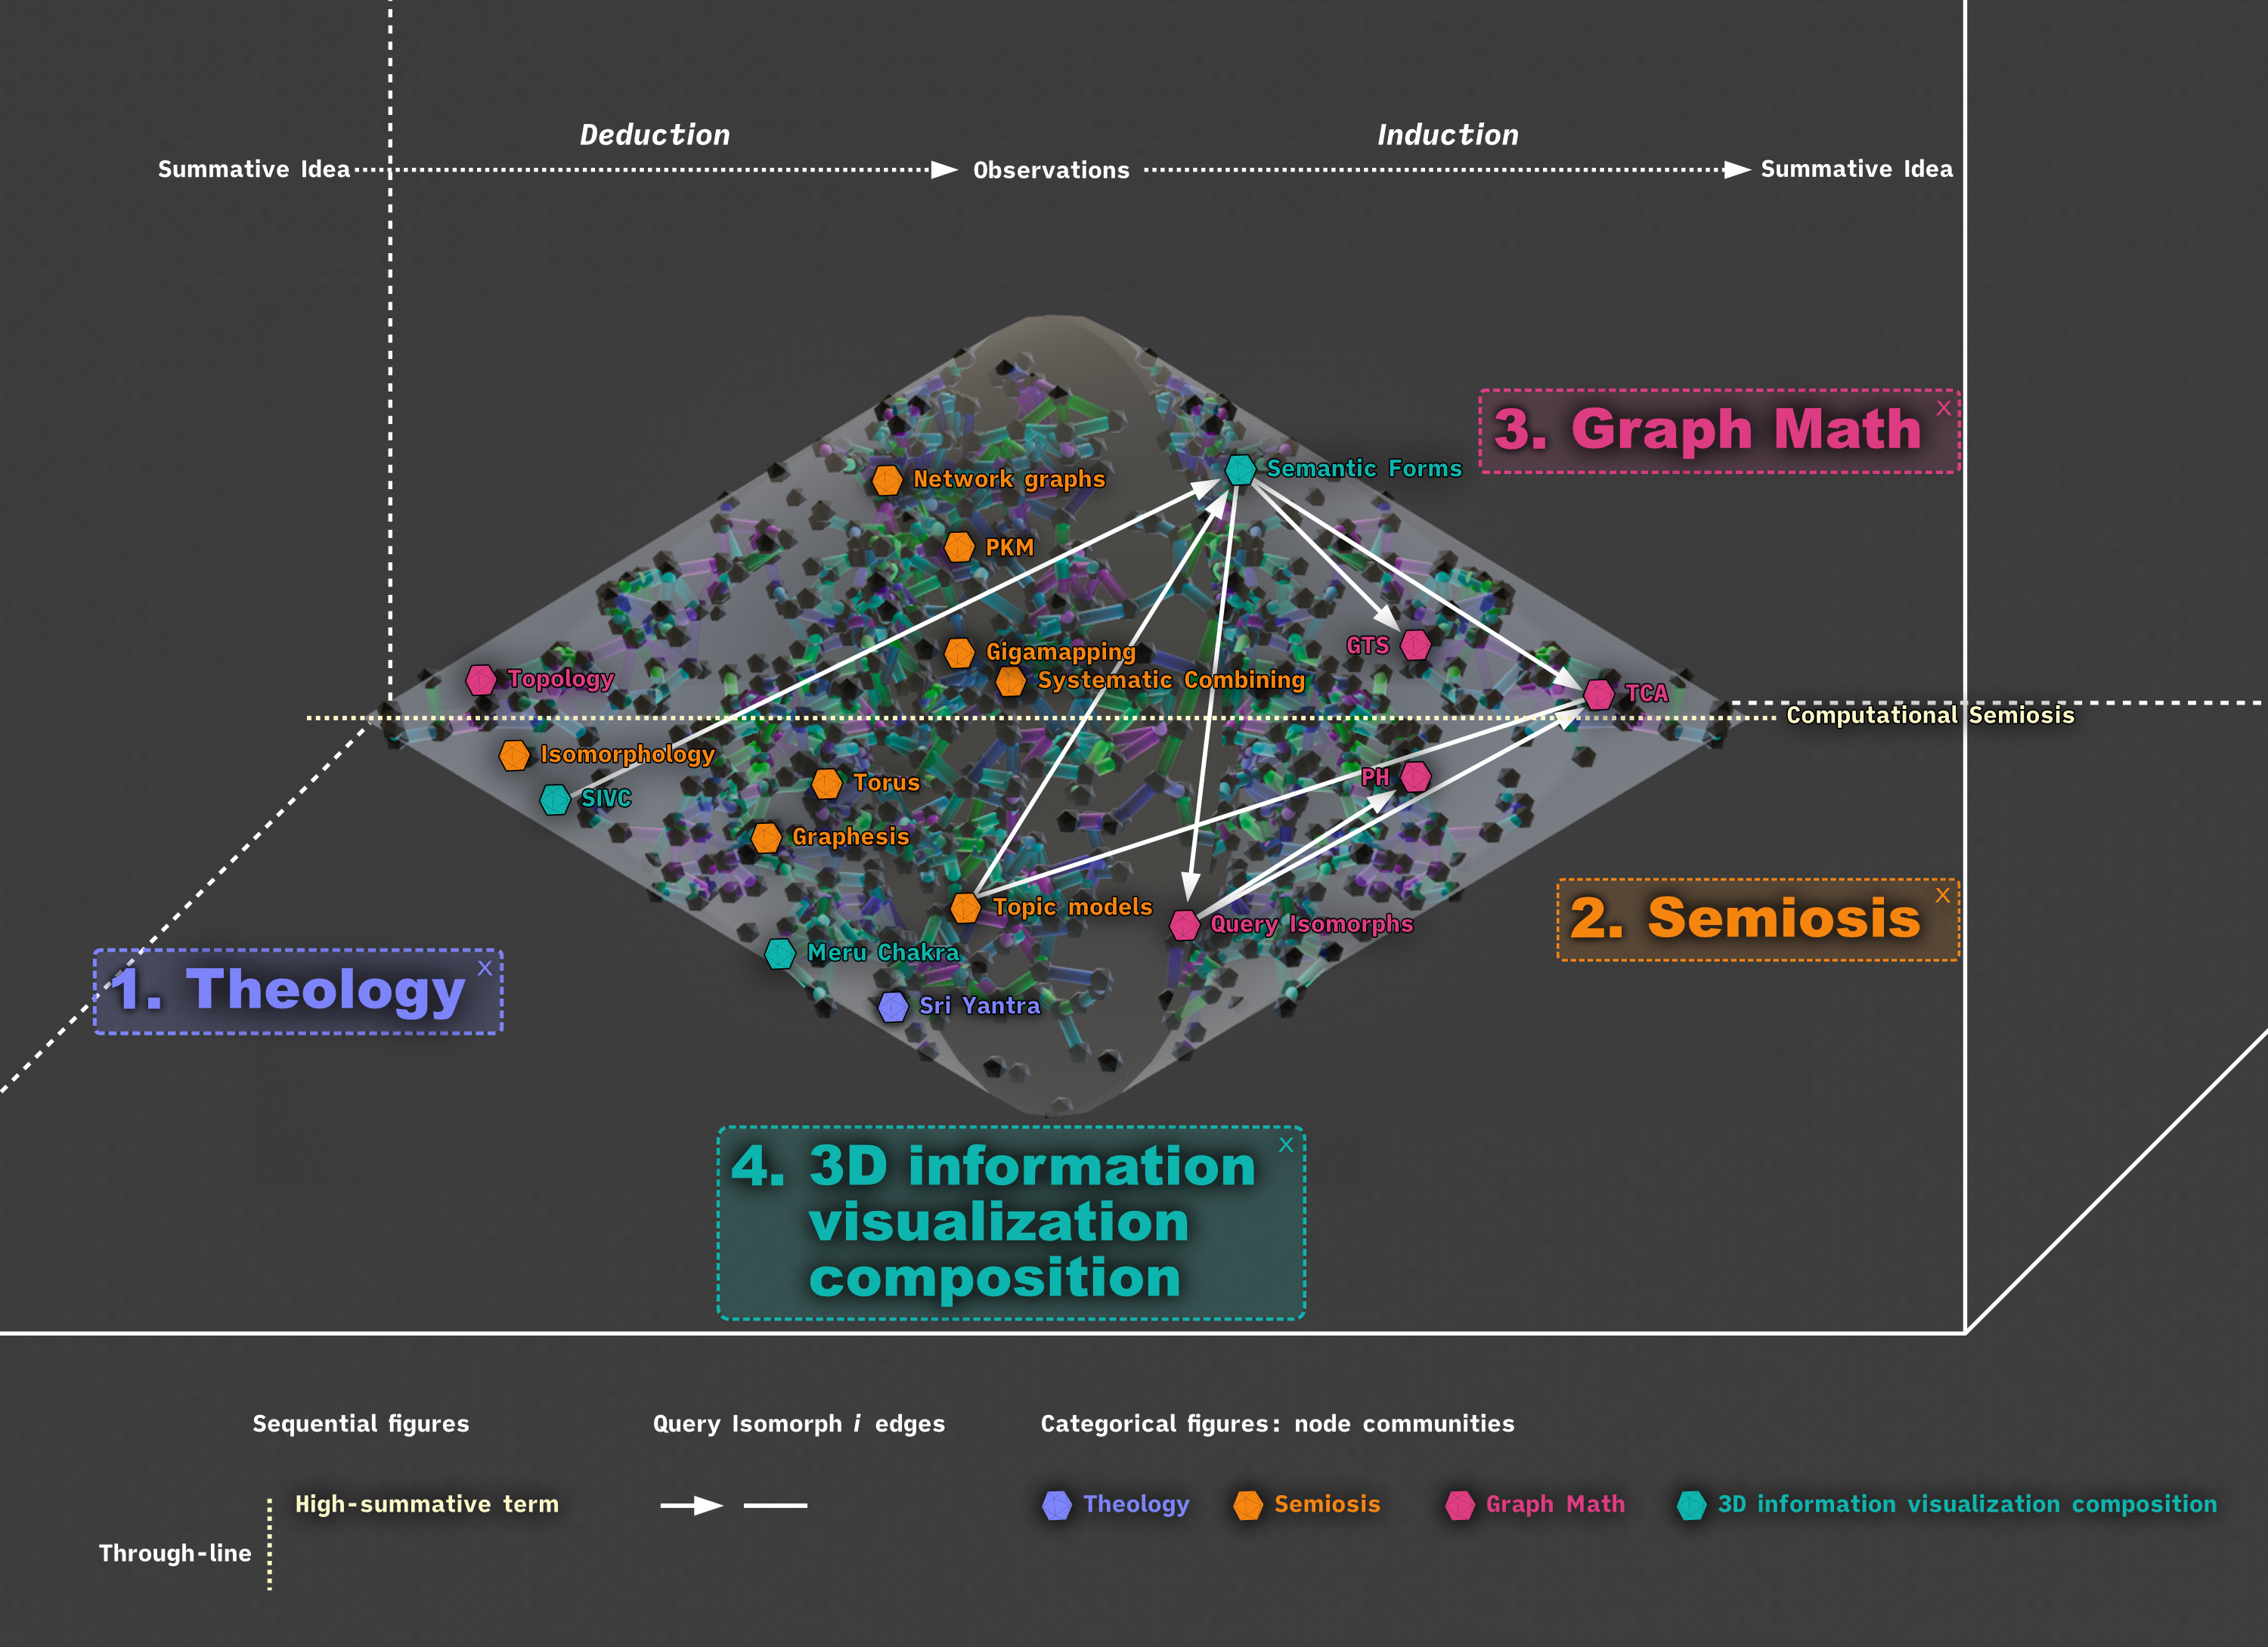
\includegraphics[width=\textwidth]{figures/5.14.DoubleCone.png}
    \caption[Double Cone Semantic Form about Query Isomorph \textit{i}]{\textbf{Double Cone Semantic Form about Query Isomorph \textit{i}.} a) Inductive direction from specific examples to ideas as categories; (b) Query Isomorph \textit{i}; (c) secondary nodes; (d) through-line analysis.}
    \label{f5.14.DoubleCone}
\end{figure}
\FloatBarrier  

The Double Cone Semantic Form in \autoref{f5.14.DoubleCone} represents the divergence of nodes in a process of deduction, and then, conversely, the convergence that occurs with deduction. My Double Cone Semantic Form for visuospatializing semantic divergence and convergence follows and builds on important precedents. As traced by Sevaldson, Pappus's (290-350) discussion of analysis and synthesis \citep[p. 7]{hinitikka_method_1974} is foundational for later visual expression including Bánáthy’s model \textit{The dynamics of divergence and convergence} \citep[p. 75]{banathy_designing_1996} and the British Design Council's Double Diamond framework \citep{design_council_history_nodate}. However, my Double Cone Semantic Form differ from these precedents as a dimensionally versatile TCA tool that visuospatializes semantic divergence and convergence for HATG and HITL CATG, compared to rather than the specifically two-dimensional model HATG models by Bánáthy and the British Design Council.
\index[people]{Sevaldson, Birger}
\index[people]{Bánáthy, Béla Heinrich}
\index[people]{Pappus}

In \autoref{f5.14.DoubleCone} I label node communities in the style of InfraNodus \citep{paranyushkin_infranodus_2019,paranyushkin_infranodus_nodate-2} \footnote{InfraNodus uses the Louvain community detection algorithm proposed by Blondel et al. \citep{blondel_fast_2008,paranyushkin_force_2022}.} Theology nodes are labelled in Purple, Semiosis terms are labelled in Orange, 3D information visualization composition terms are labelled in Teal, and Graph Math terms are labelled in Orange.

\noindent  \textbf{Query Isomorph \textit{i} in the Sphere and Horn Torus Semantic Forms} 
\\
\textbf{\textit{Sphere Semantic Form}}

\FloatBarrier  
\begin{figure}[h!]
    \centering
    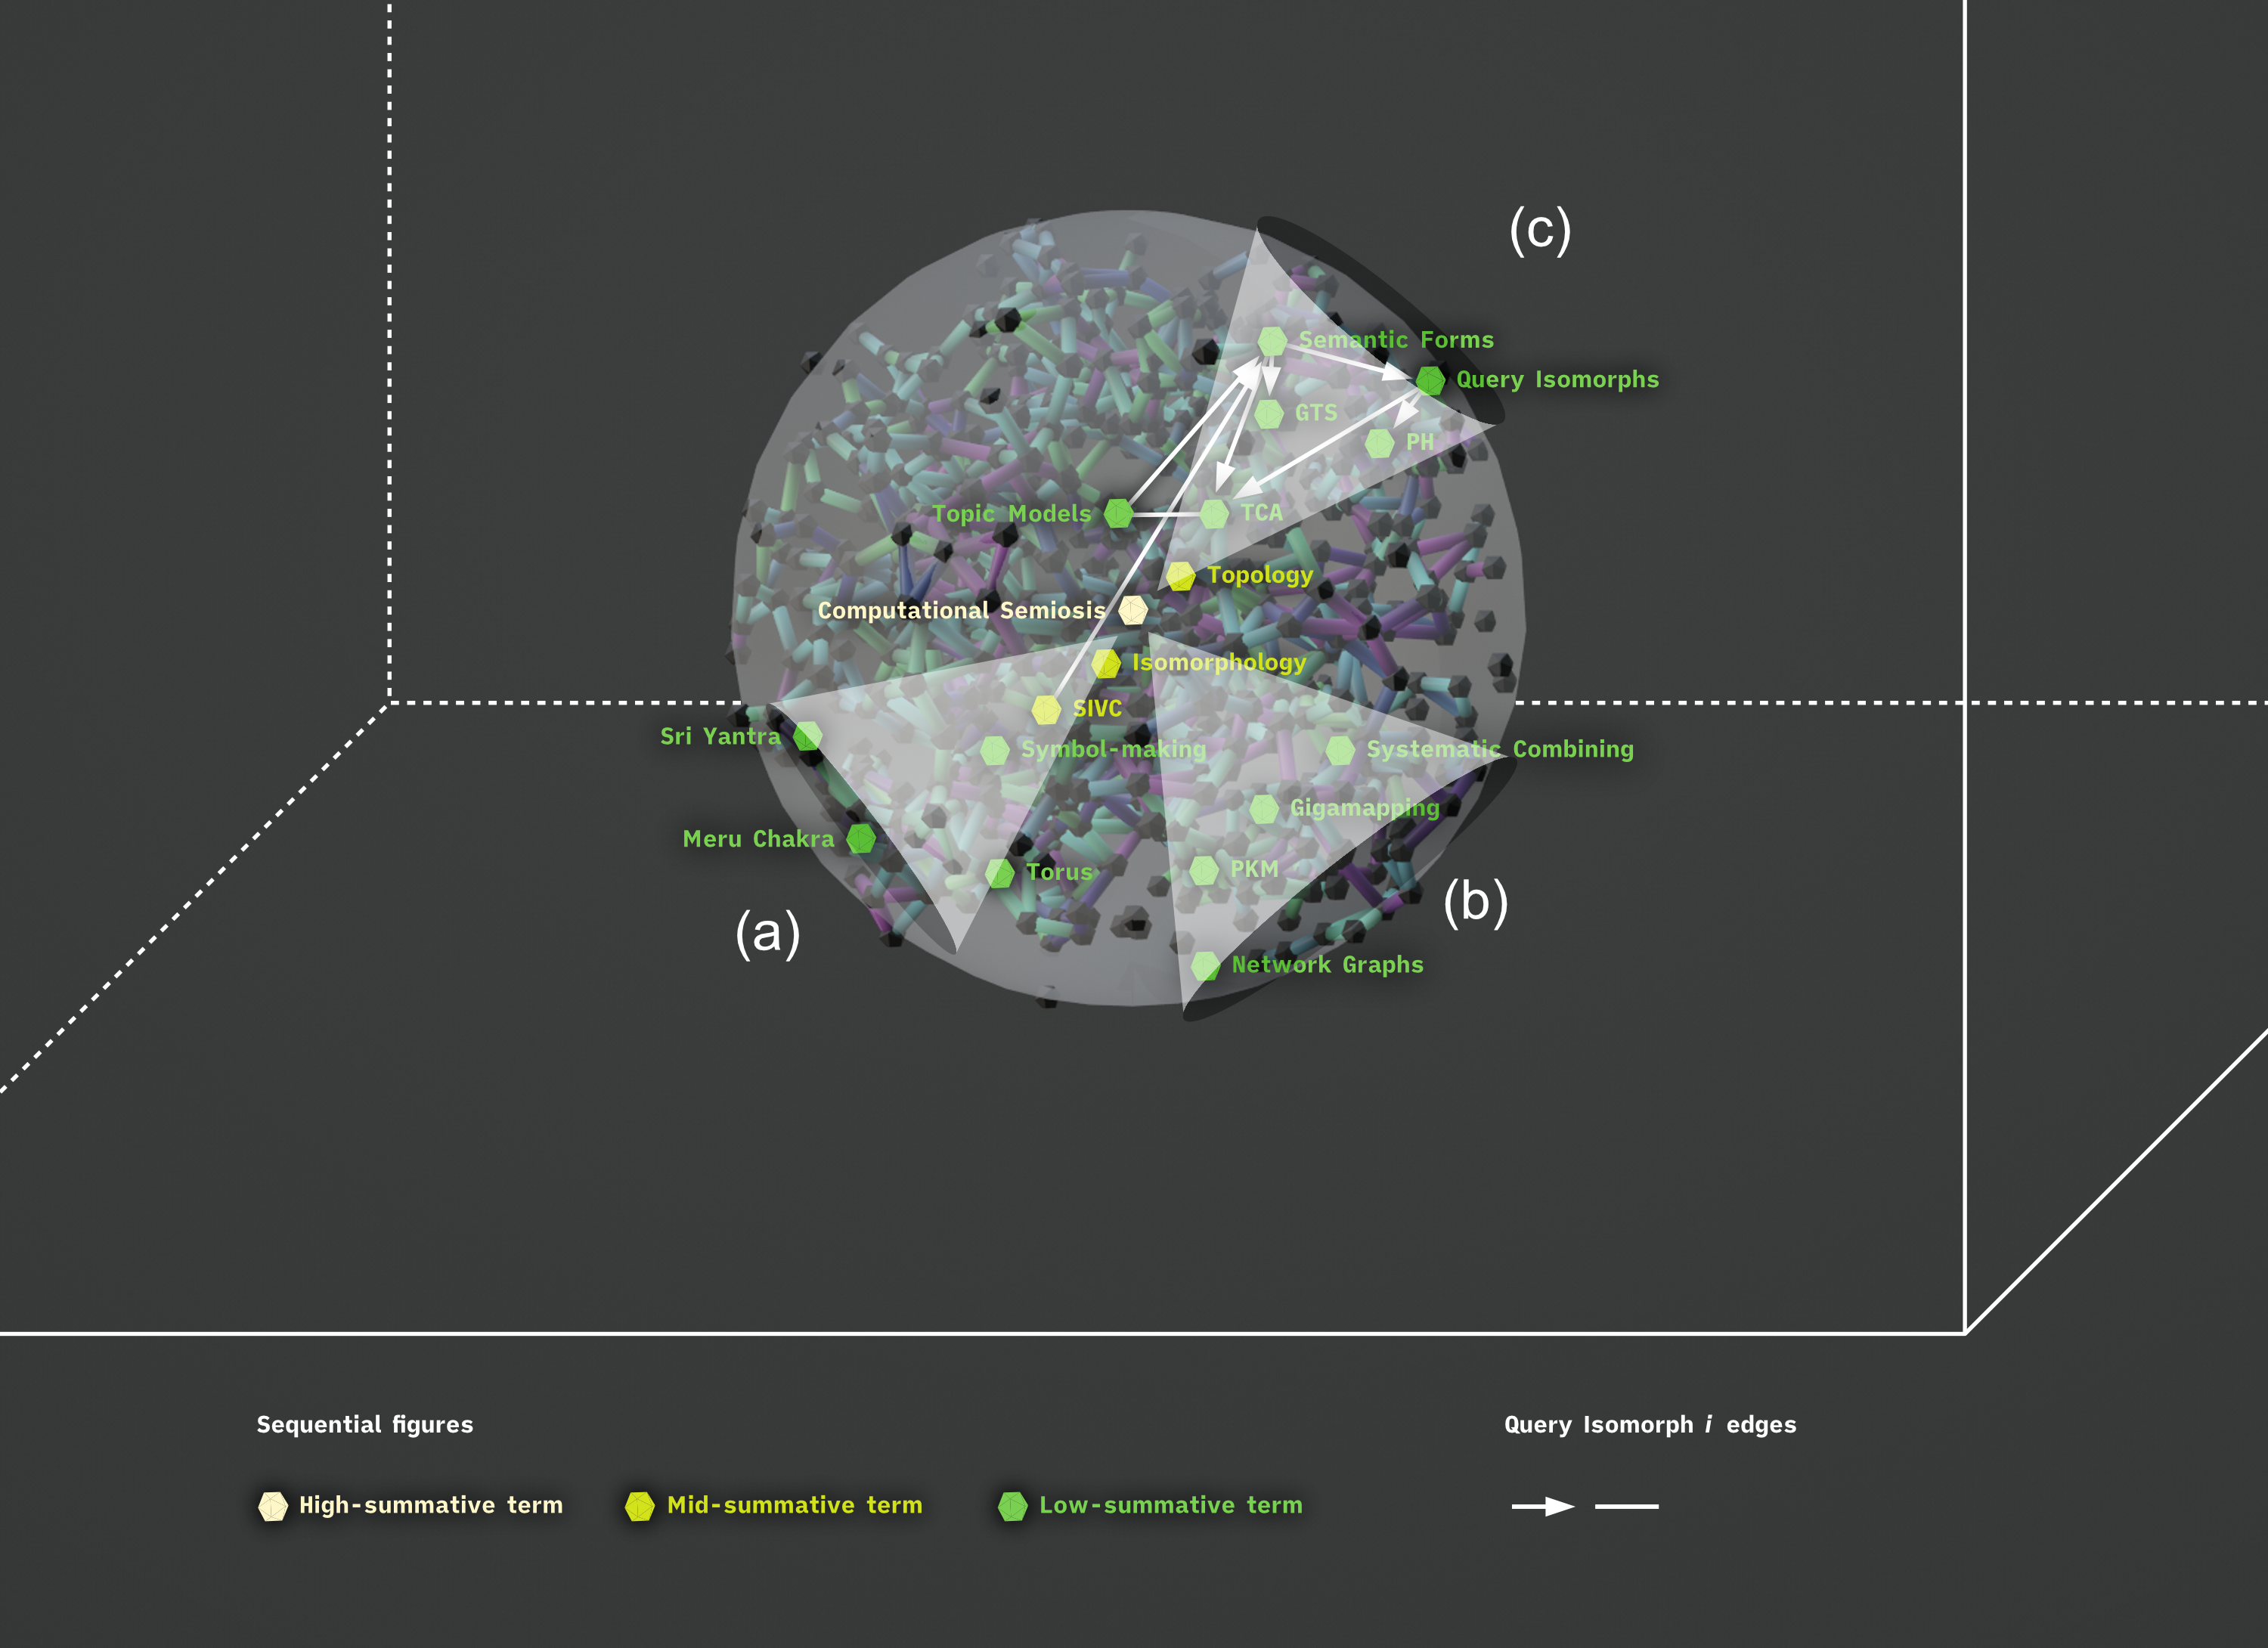
\includegraphics[width=\textwidth]{figures/5.15.Sphere1.png}
    \caption[Sphere Semantic Form about Query Isomorph \textit{i}]{ \textbf{Sphere Semantic Form about Query Isomorph \textit{i}}}
    \label{5.15.Sphere1}
\end{figure}
\FloatBarrier  

The Sphere Semantic Form is similar to the Cone Semantic Form in that it represents hierarchical relationships between nodes. However, while the Cone Semantic Form can represent various hierarchies within itself, it is predominantly a representation of one hierarchy. The Sphere Semantic Form increases the number of hierarchies that can be represented by effectively representing multiple Cone Semantic Forms. 

\autoref{5.15.Sphere1} illustrates how the high-summative node Computational Semiosis is shared by three Cone Semantic Forms: (a) which is about Spatial Information Visualization Composition and Isomorphology, (b) which is about text graph methods of visuospatial knowledge production, and (c) which is about Topology.  

I present the Sphere Semantic Form with nested Cone Semantic Forms to illustrate an additional notation method for grouping nodes that does not depend on colour encoding like in \autoref{f5.14.DoubleCone}. In the same way that the Circle Semantic Shape can contain and overlap with Triangle and Circle Semantic Shapes, like in the Obsidian knowledge graph in \autoref{f5.2}, the Sphere Semantic Form can nest and overlap with Cone and Sphere Semantic Shapes. The number of nodes that can be organized in nested hierarchies of Semantic Forms, then, is substantially more than the nodes that can be represented in a Circle Semantic Shape. I expect that testing node hierarchies of Semantic Forms versus Semantic Shapes will reveal results consistent with Ware and Mitchell's \textit{Visualizing graphs in three dimensions} \citep[p. 10]{ware_visualizing_2008}. 

\noindent \textbf{Horn Torus Semantic Form}

\FloatBarrier  
\begin{figure}[h!]
    \centering
    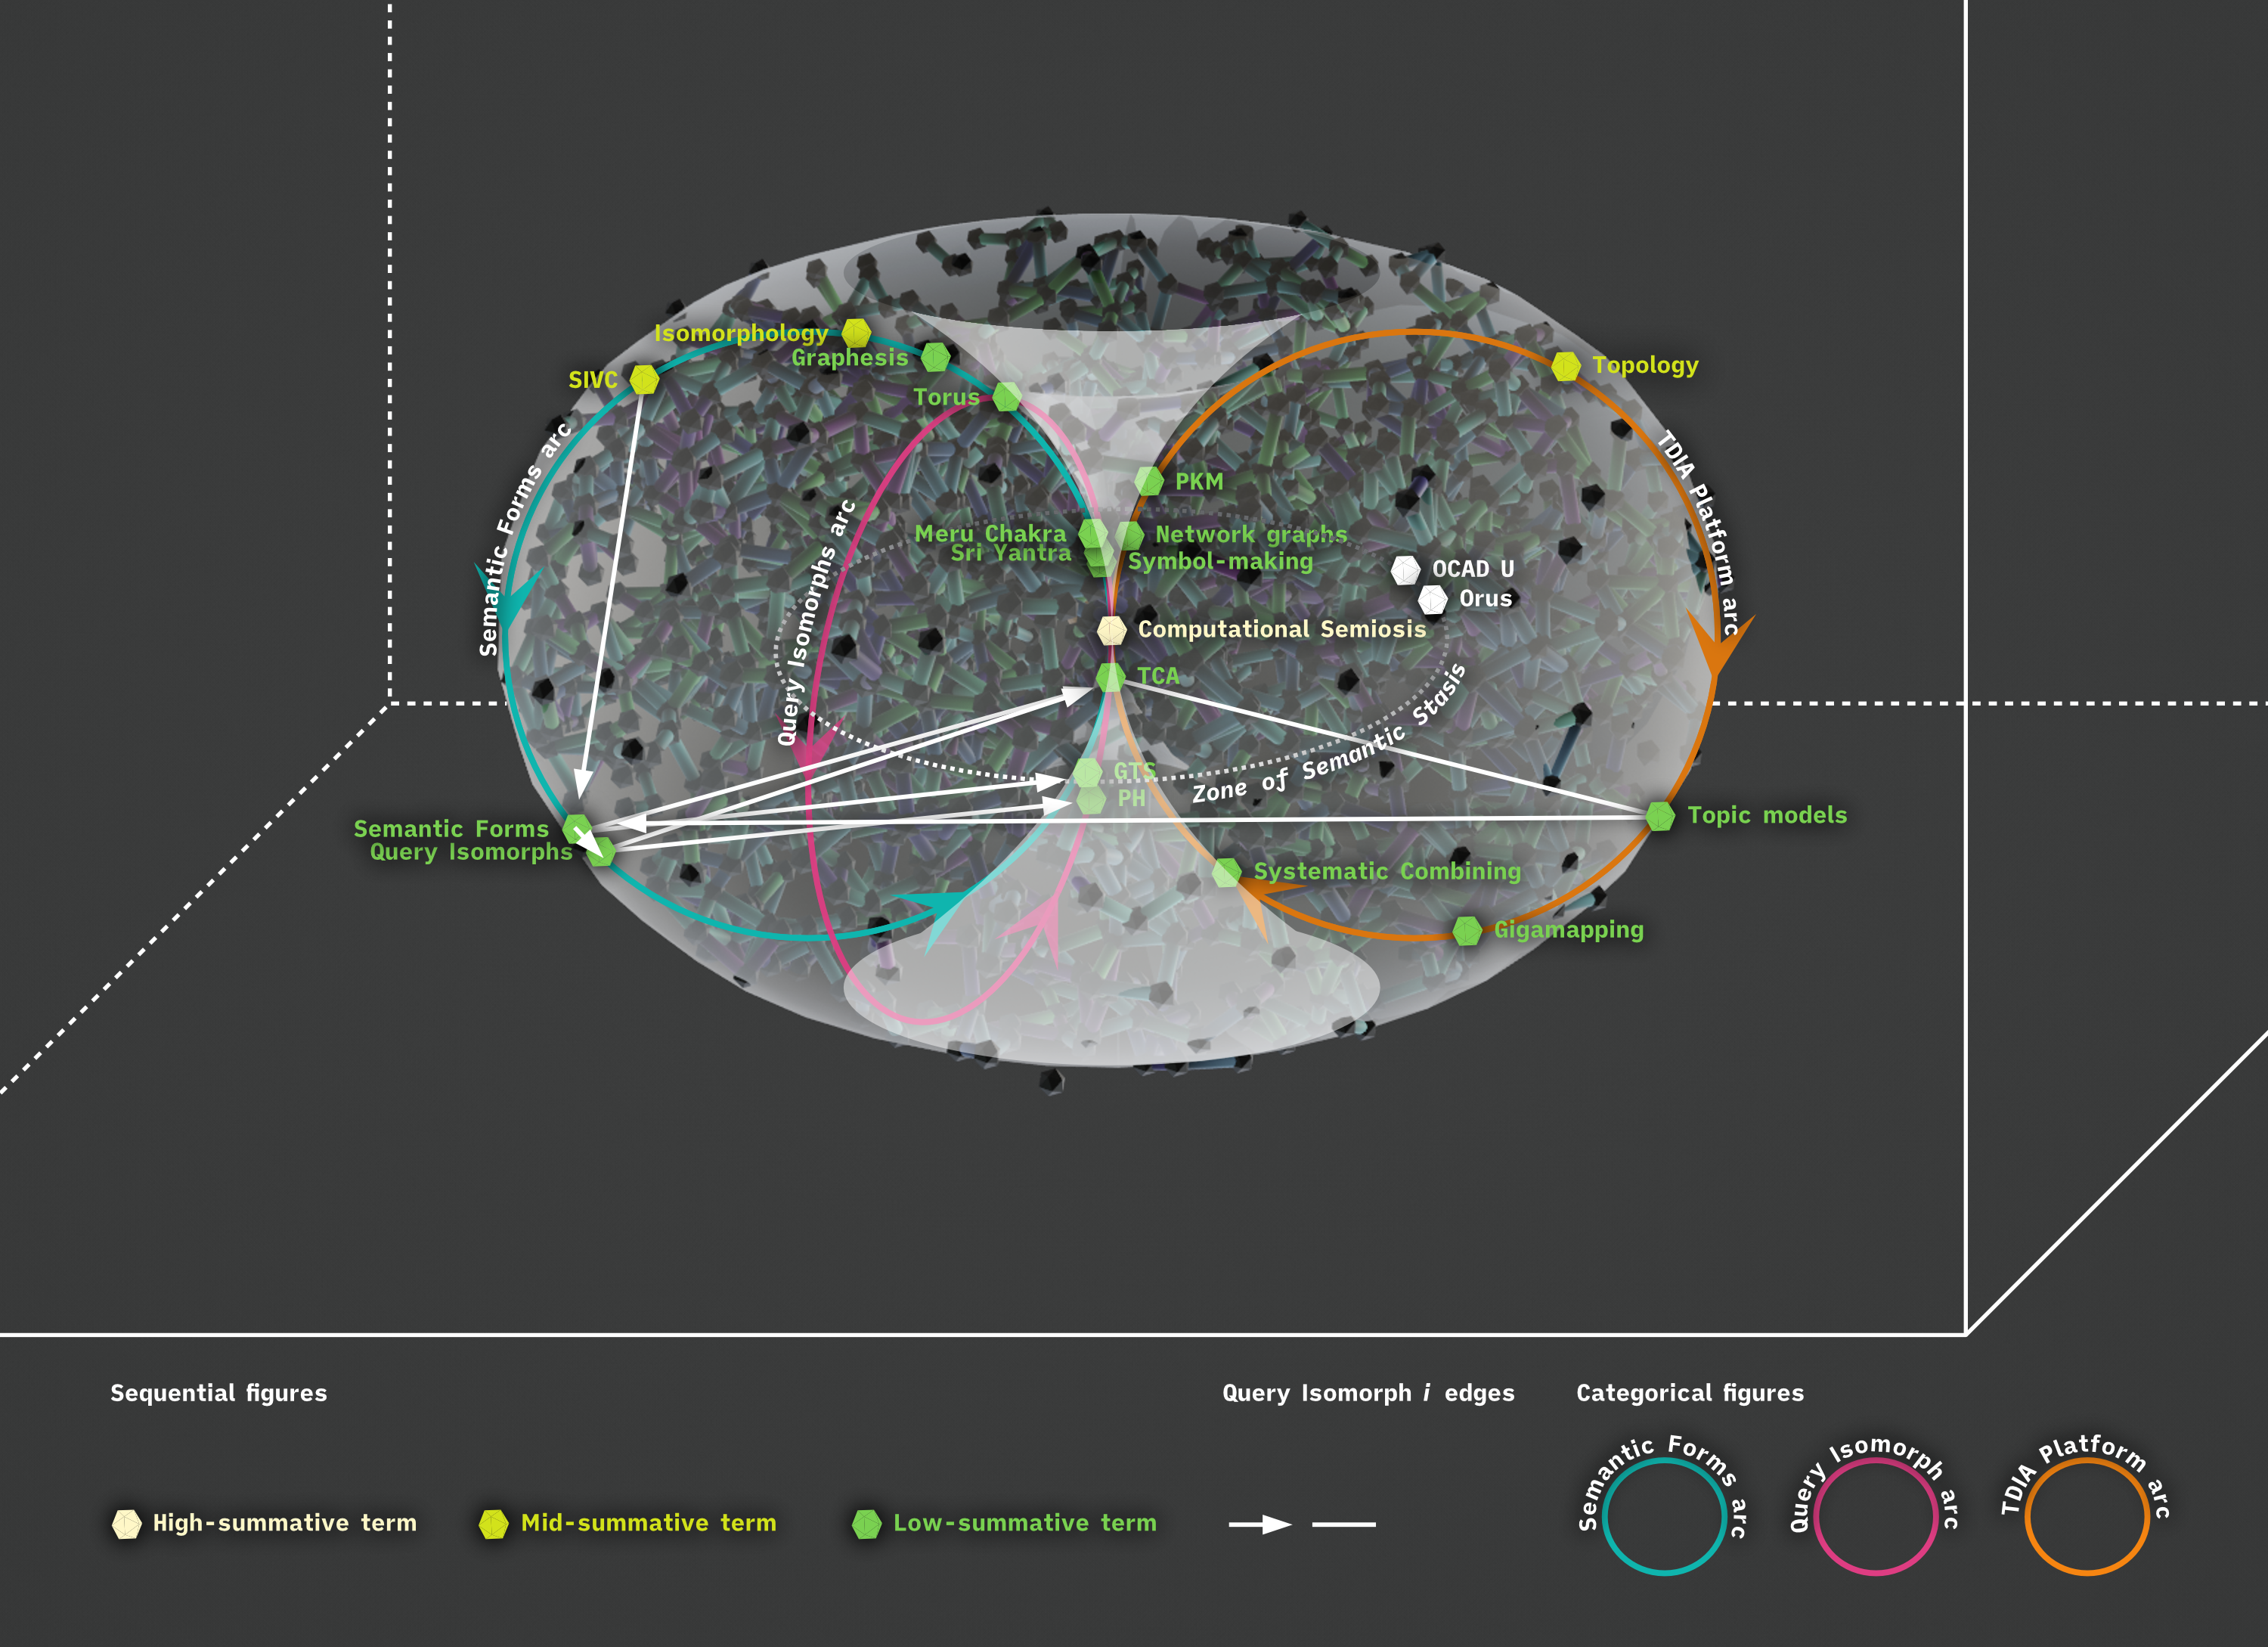
\includegraphics[width=\textwidth]{figures/5.16.HT2.png}
    \caption[Horn Torus Semantic Form about Query Isomorph \textit{i}]{Horn Torus Semantic Form about Query Isomorph \textit{i}.}
    \label{f5.16.HT2}
\end{figure}
\FloatBarrier  

The Horn Torus Semantic Form is similar to the Ring Torus and Cylinder Semantic Forms in that it represents a series of Circle Semantic Shapes like Rolodex \citep{mellby_my_2021} of Obsidian or Logseq graphs in one continuous space as the tube of its body. However, the inner radius of the Ring Torus narrows to a single highly-summative point in the centre of the Horn Torus Semantic Form, similar to a Sphere Semantic Form, which also forms two Cone Semantic Forms, diverging away from each other in the negative space of the Horn Torus. Furthermore, the Loop-line of the Ring Torus Semantic Form is a Zone of Semantic Stasis in the Horn Torus Semantic Form; as opposed to having the core of the torus tube be a zone of high-summativeness or high semantic connectedness, I model the Horn Torus Semantic Form as a representation of the tree, whereby the base of the tree's trunk reaches up and out into branches, whose leaves fall and transform into soil, whose nutrients are taken up by the tree's roots, back to and from the re-origin point of the tree's trunk in an ongoing cycle of blossoming transformation.

I depict these Horn Torus Semantic Form trajectories of transformation as arcs emerging and returning to their re-origin point. Similarly to the Ring Torus I used \autoref{f5.11.Time circle} to accurately place term nodes from semantic field \textit{S} onto their respective arcs. The re-origin point Computational Semiosis is in the high-summative sequential figure colour Light yellow. I depicted the transformation trajectory arcs by labelling them in categorical figure colours: the Semantic Forms arc in teal, the Query Isomorph arc in magenta, and the TCA Platform arc in orange. My transformation trajectory arcs follow the circumference of the torus tube like Rucker's vertical arc orbits representing time in his horn torus model of space-time \citep{rucker_infinity_2005}. However, my transformation trajectory arcs move upward and out from the horn torus's centre. 

The Horn Torus Semantic Form differs from the Sphere Semantic Form because it does not nest a variety of Cone Semforms within it in different angles. In fact the two Cone Semantic Forms at the poles of the Horn Torus Semantic Form represent a Gestaltian geometric liminality and interbeing \citep[p. 80]{nhat_hanh_world_2008}  \citep[p.25]{deleuze_thousand_2007} of Semantic Form in which the Cone Semantic Form and the Ring Torus Semantic Form are exactly at the brink of being their own forms, being each other, and being a whole that ``is other than the sum of its parts."  \citep[Koffka in Sevaldson, p. 163]{sevaldson_designing_2022}. This thesis is in many ways a celebration of the strange and wonderful qualities of the horn torus as spatial information visualization composition, particularly as network graph isomorph.

\FloatBarrier  
\begin{figure}[h!]
    \centering
    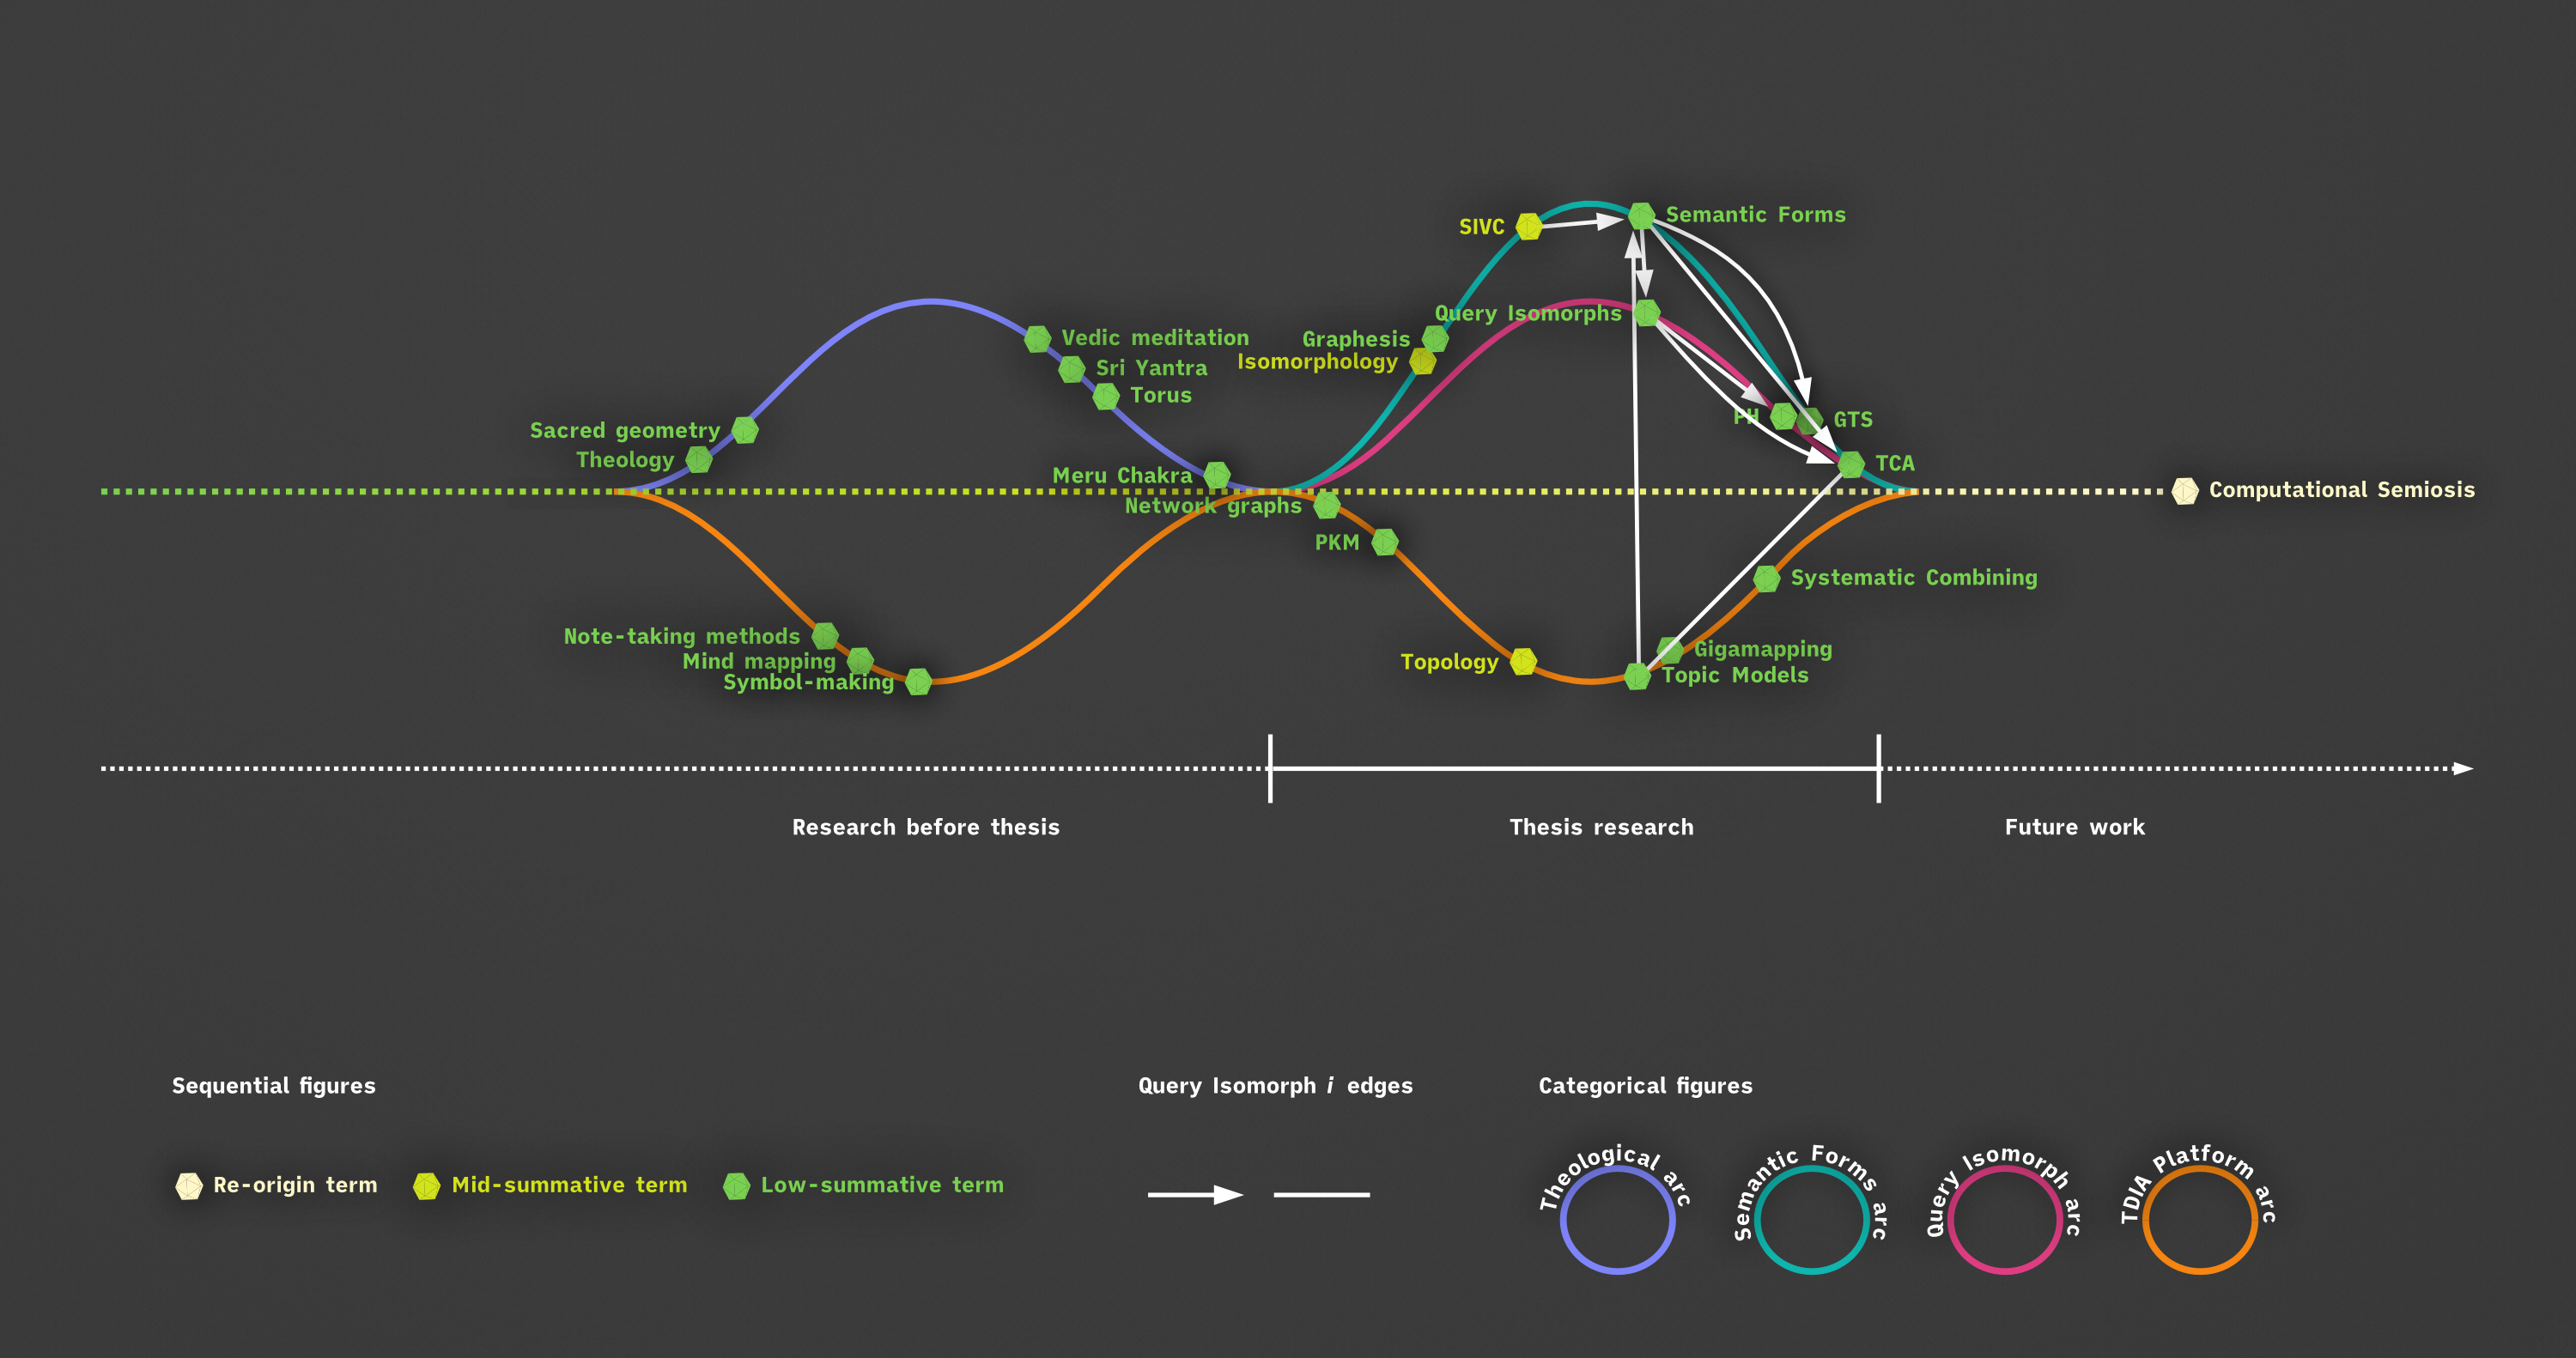
\includegraphics[width=\textwidth]{figures/5.17.HT3.png}
    \caption[Horn Torus Semantic Form about Query Isomorph \textit{i}: dimensionally reduced to 2D]{Horn Torus Semantic Form about Query Isomorph \textit{i}:dimensionally reduced to 2D.}
    \label{f5.17.HT3}
\end{figure}
\FloatBarrier  

In \autoref{f5.17.HT3} I illustrate two sequences of Horn Torus Semantic Form re-origination in a dimensional \textit{reduction} of \autoref{f5.16.HT2}. On the left I represent the research before my graduate work at OCAD U in a cycle of divergence and convergence. To the right I represent my thesis research at OCAD U, which leads out to future work. I represent  Query Isomorph \textit{i} by connecting its nodes with white colour edges. The three transformation trajectory arcs from \autoref{f5.16.HT2} are included, but left of the bracket for Thesis research I added arcs to represent a rough timeline of encountering key formative ideas: First, I added a Theological arc which includes the terms Theoloy, Sacred geometry, Vedic meditation, Sri Yantra, and Torus. Note here that the Torus is included earlier in this representation because my fascination with it began with artistic representations of chakras as horn tori. Also note that the Meru Chakra is placed right before the beginning of my thesis research arcs, and right before Network graphs. I labelled the Theology arc Purple, the Semantic Forms arc Teal, and the Query Isomorphs arc Magenta because I arrived at a study of network graphs through my fascination with the Meru Chakra. Since the development of Semantic Forms and Query Isomorphs are distinct extensions of, and disambiguations of, a theological principle, I used colour to represent how the Teal Semantic Forms arc and the Magenta Query Isomorphs arc are the separation of blue and red primary colours that make up Purple. Second, the TCA Platform arc extends backward into a short origin story including Note-taking methods, Mind mapping  \citep{buzan_ultimate_2005}, and Symbol-making. Both arcs, additions left of my Thesis research arcs represent a rough timeline as I mentioned. I spread each idea along the timeline according to my estimated age for when I encountered each idea. Nodes furthest left on the timeline represent the earliest ideas which influenced this research, and the nodes closest to the beginning of my Thesis research arcs represent the ideas that were most influential right before beginning my degree here at OCAD U. 
\section{Contribution 7. TCA Workspace, for living webs of thought}
\FloatBarrier  
\begin{enumerate}
      \item[\textbf{C7}] \textit{TCA Workspace}, a proposal for a collaborative HITL CATG + HATG platform to:
    \begin{enumerate}
        \item[(a)] house all my thesis contributions (\textit{Semantic Forms}, \textit{Query Isomorphs}, \textit{OSNS}, \textit{Symbol-setting}, \textit{TTG}, and \textit{TCA Researcher Grouping}).
        \item[(b)] facilitate their combined use with Systemic Design methods for visuospatial reasoning discovered through my literature review, such as gigamapping \citep{sevaldson_giga-mapping_2011}, \citep[p.~26]{sevaldson_designing_2022} and Systematic Combining \citep[p.~554]{dubois_systematic_2002}, \citep{kjode_entanglement_2024}.
    \end{enumerate}
\end{enumerate}
\FloatBarrier  
\index[terms]{Systemic Design}
\index[terms]{gigamapping}
\index[terms]{Systematic Combining (SC)}


TCA Workspace is my proposal for a software platform which will accelerate the computational analysis of texts and graphs with Semantic Forms, Query Isomorphs, Symbol-setting, Ontological Semantic Network Graphs, and Terroir of Text and Graphs (TTG) as independent tools or as combined approaches. The ‘space’ in TCA Workspace invokes the dimensionality of ‘place’, but invokes the colliding of electromagnetic particles in nested holarchies of complexity, from the atoms that are our words, to the ontologies that are our visible universe. In this sense, TCA Workspace is a particle accelerator of ideas that activates living webs of thought.
\index[terms]{TCA Workspace}

In TCA Workspace researchers would examine isomorphogenic molecular dynamics simulations of ‘datacules’, formed of spatial network graphs of entities and relationships in Query Isomorphs and Semantic Forms. Researchers would be able to identify and observe the semantic forces at play in text and graphs, using the rich analogues available from the consilient fields of physics and chemistry, and computational analysis from perhaps the most consilient field of mathematics using Topological Capta Analysis. Doing so is a means of identifying richer meta-patterns in the visual forms of knowledge production we use, and developing new language for Sustainability Transitions, syntopically consilient or perhaps beyond it. 
\index[terms]{TCA Workspace}

The following are evidence for how current approaches to graphs and text are aligned with the TCA Workspace toolkit, and can be expanded by it. 

\subsection{Dimensional addition in Systems Oriented Design}
Considering the Meta-Systematic Combining approach I used in this thesis for arriving at Semantic Forms through dimensional addition of Semantic Shape, I propose dimensional addition to Sevaldson’s gigamaps \citep{sevaldson_giga-mapping_2011,sevaldson_designing_2022} as a feature of TCA Workspace that can work concurrently with Semantic Forms and Query Isomorphs. As introduced in \autoref{f5.9.Semantic Shape Circle} with the spatial TCA Workspace representation of the Circle Semantic Shape PKM graph with an overlay of Query Isomorph nodes, I do not intend to represent information in only two-dimensions or three-dimensions in TCA Workspace; instead, I think both can be valuable together in the same render. To illustrate my the dimensional versatility of the interface of TCA Workspace, I present two examples of visuospatial gigamaps: \autoref{f5.30.HT gig} my Horn Torus Semantic Form gigamap and \autoref{f5.31.Cone gig} my Cone Semantic Form gigamap.
\clearpage

\subsubsection{Gigamaps with Semantic Forms}
\FloatBarrier  
\noindent  \textbf{Horn Torus Semantic Form gigamap}
\\
\begin{figure}[h!]
    \centering
    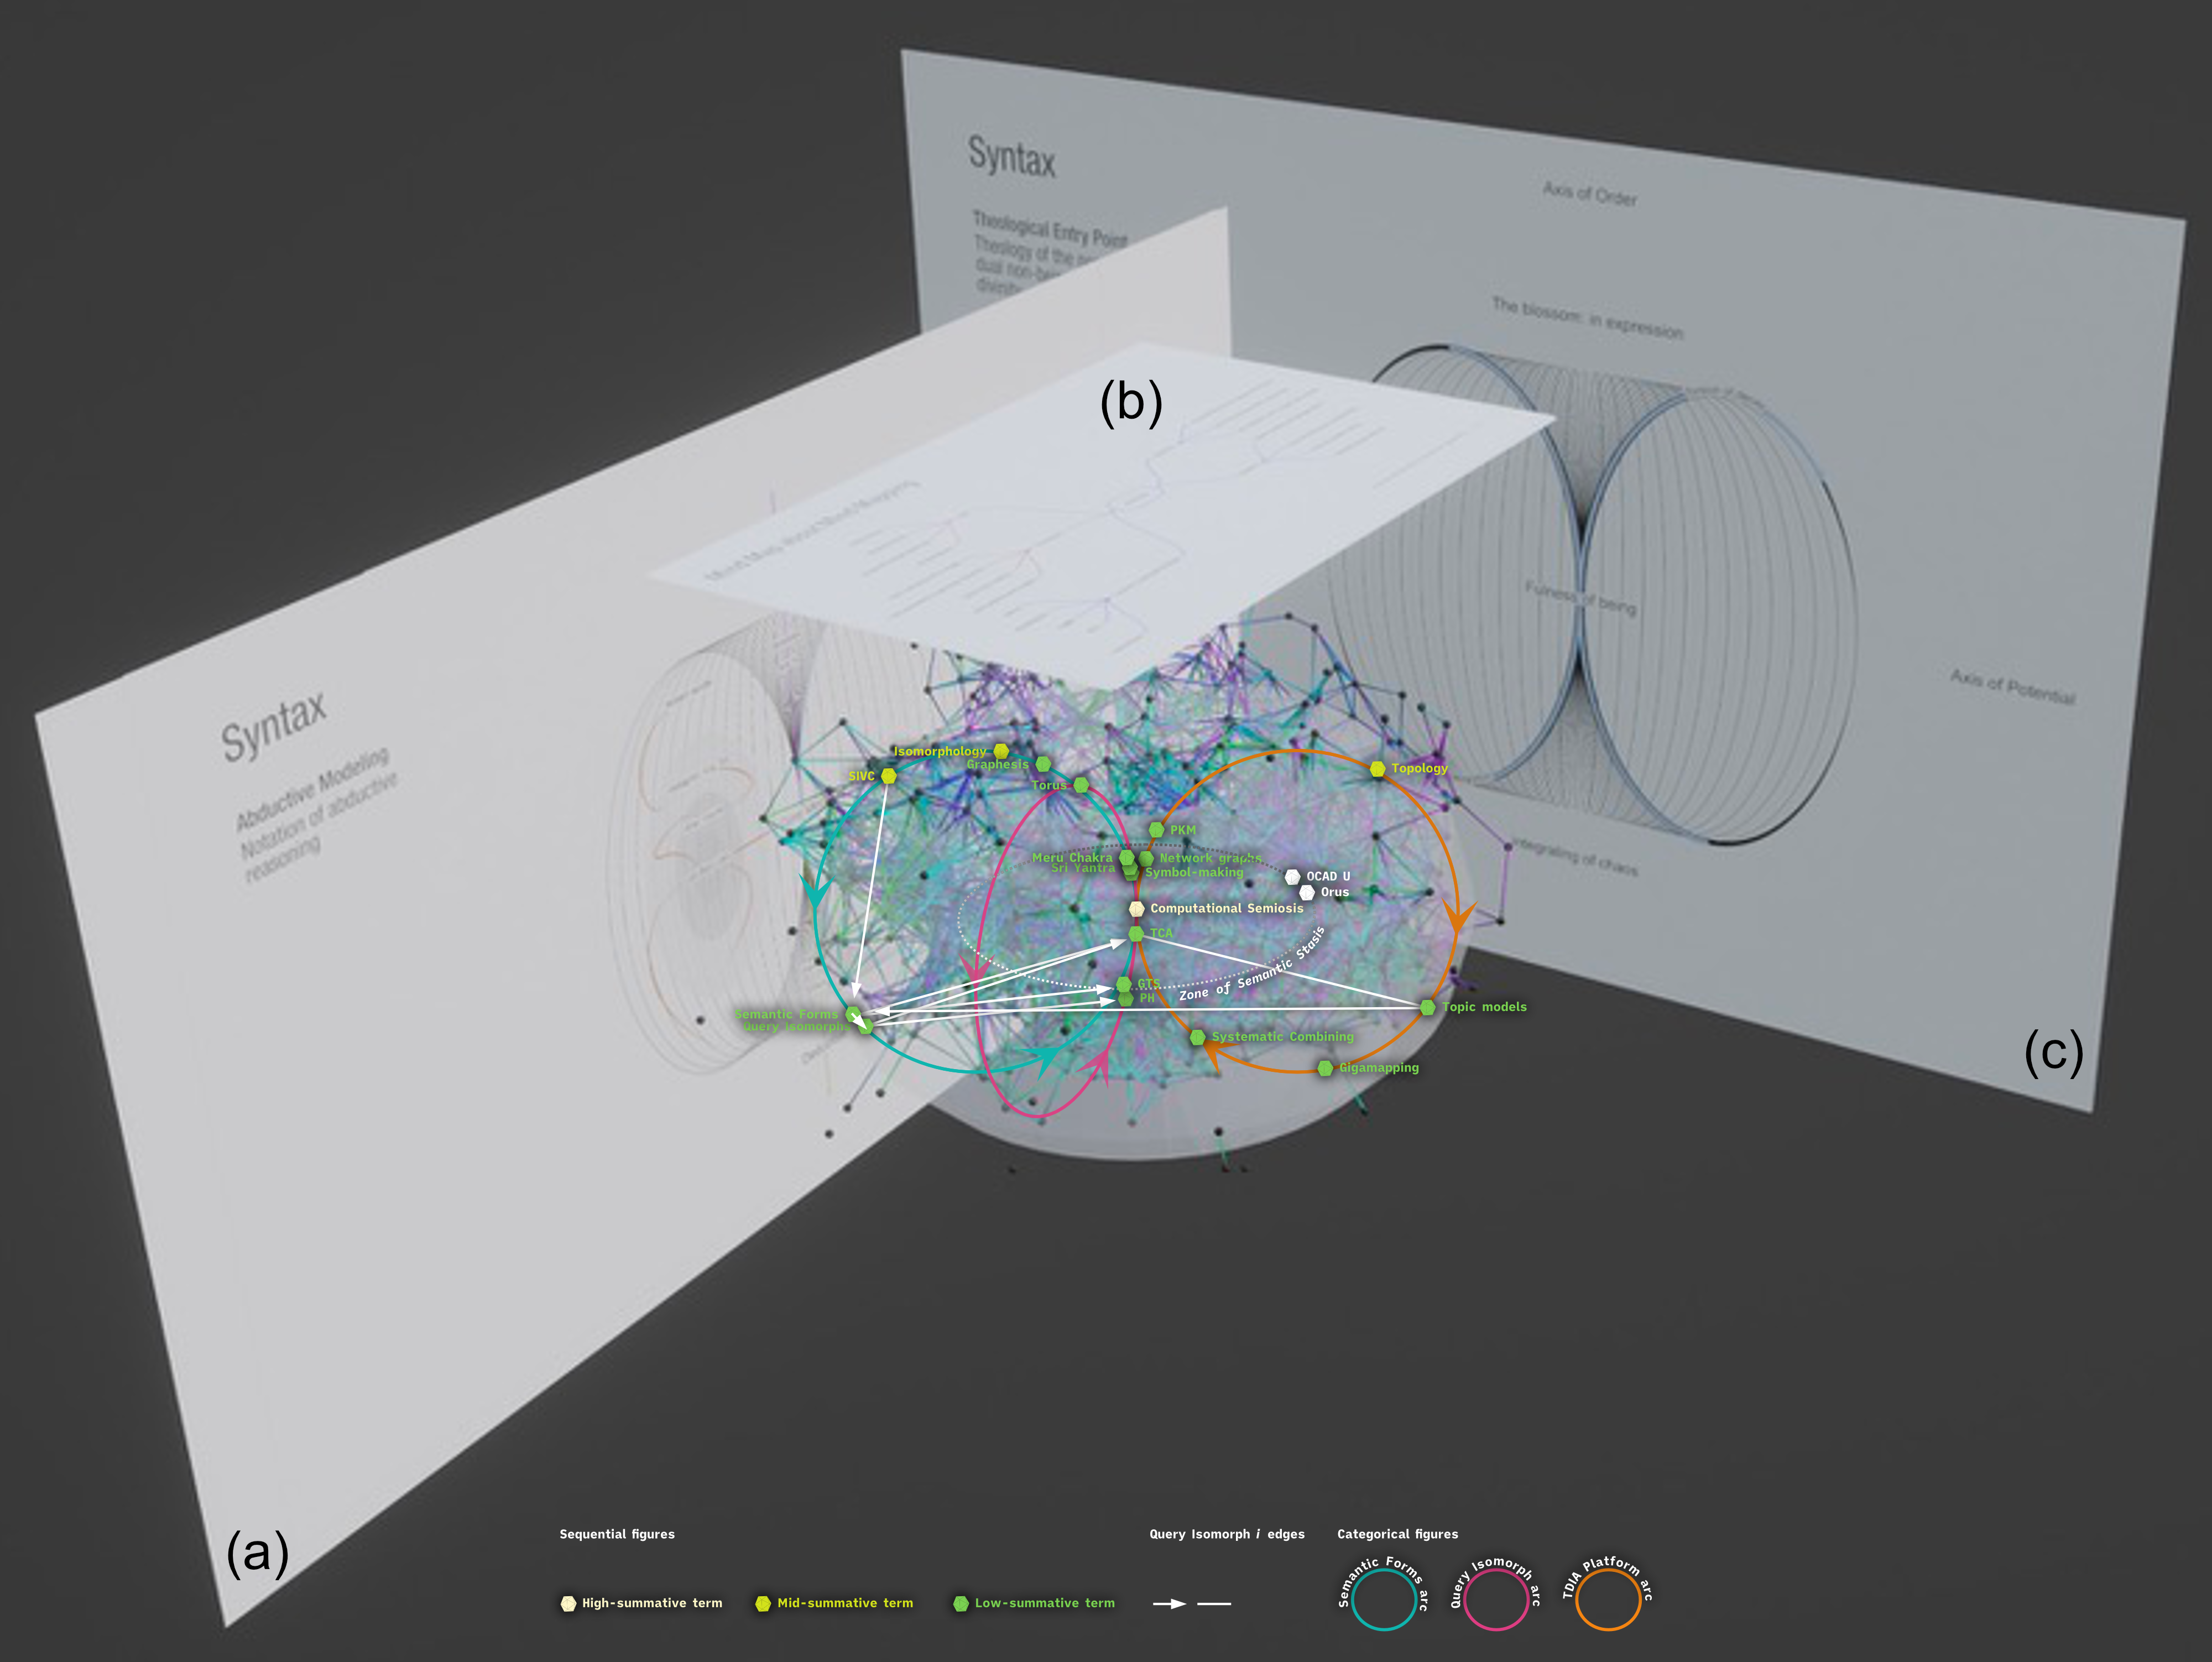
\includegraphics[width=\textwidth]{figures/5.30.HT gig.png}
    \caption[Horn Torus Semantic Form gigamap]{\textbf{Horn Torus Semantic Form gigamap.}}
    \label{f5.30.HT gig}
\end{figure}
\FloatBarrier  

First, in \autoref{f5.30.HT gig}, Horn Torus Semantic Form gigamap,I depict a conceptual gigamap with a Horn Torus Semantic Form network graph along with dimensionally reduced two-dimensional panes. In (a) and (b) I depict the two-dimensional panes which reveal the Disintegration and Integration arcs from \autoref{f4.1} that organize the semantic relationships of divergence and convergence from \autoref{f5.16.HT2}. In (c), I depict the Horn Torus Semantic Form from its top view as a Mind Map \citep{buzan_ultimate_2005} as an example of more conventional dimensional reductions into Circle Semantic Shapes. Angles for panes (a), (b), and (c), were chosen for simplicity of introduction. The angles of a two-dimensional reduction of a given Semantic Form would be positioned in as many ways as there are vantage points. In fact, the diversification of dimensional reduction angles can empower HITL CATG by summarizing the most influential vantage points. HATG  from various angles would permit a researcher to examine a spatial network graph with their own pattern-finding abilities.




\noindent  \textbf{Cone Semantic Form gigamap}
\\
\FloatBarrier  
\begin{figure}[h!]
    \centering
    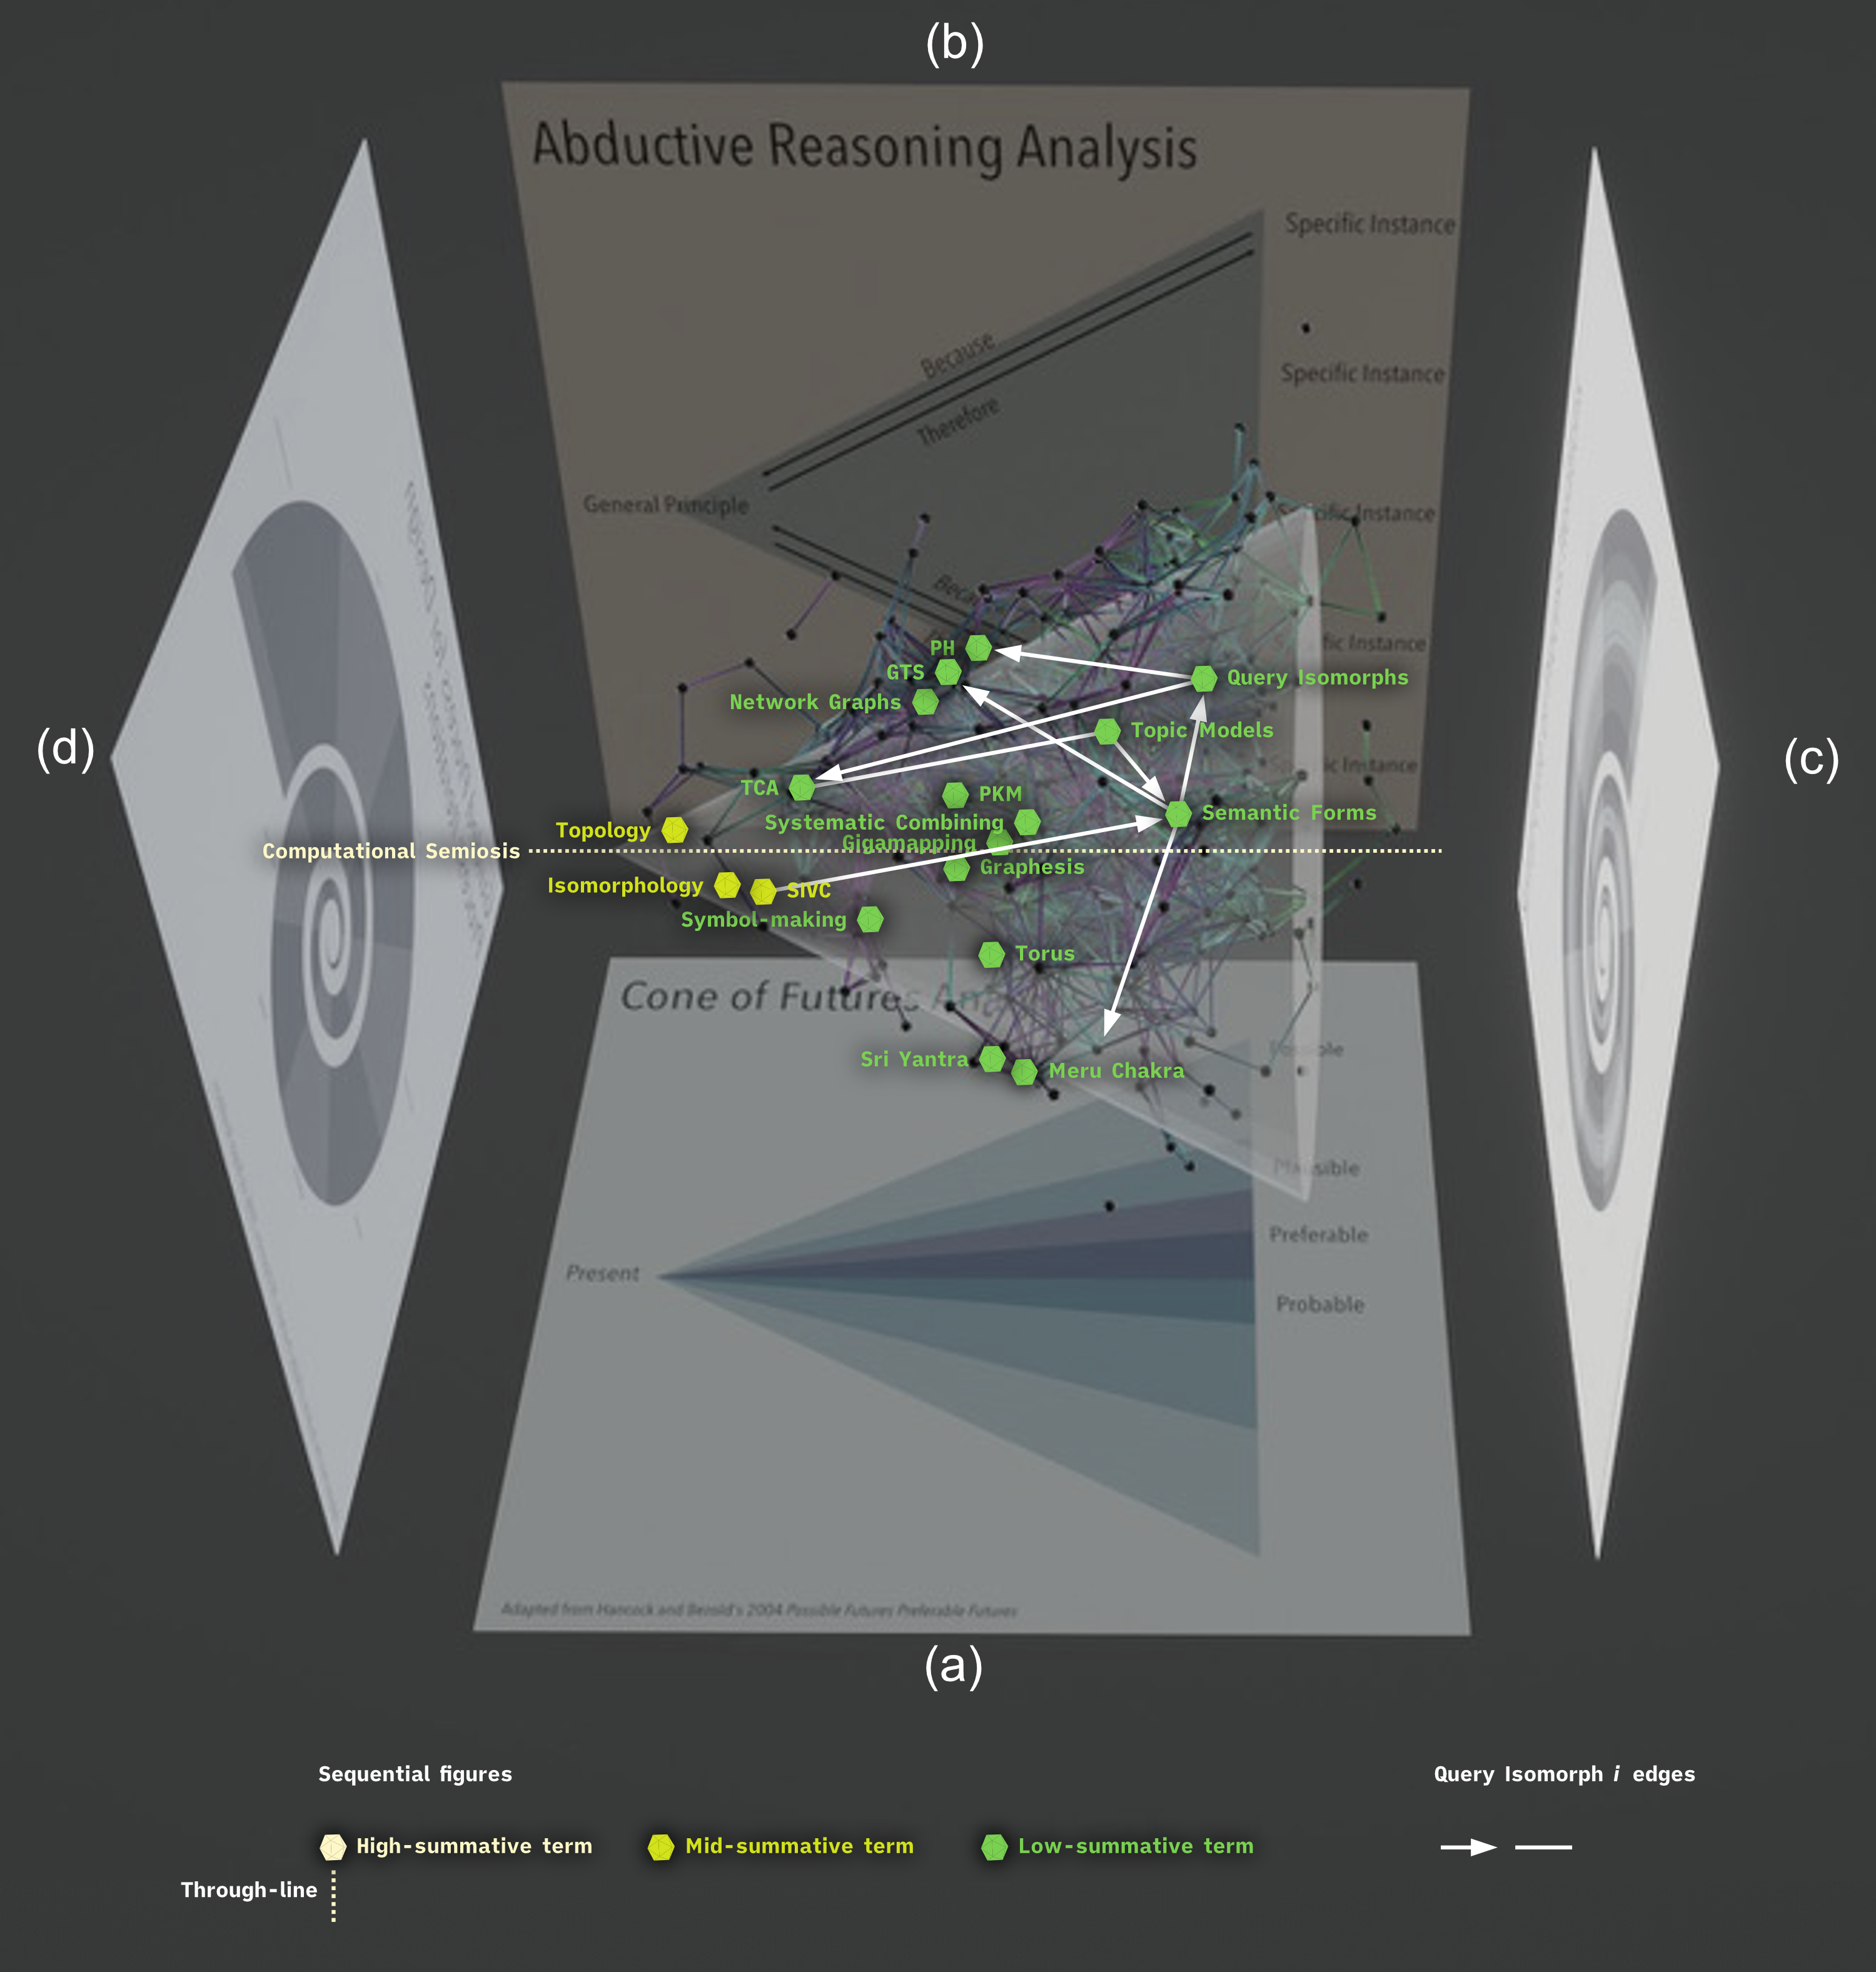
\includegraphics[width=\textwidth]{figures/5.31.Cone gig.png}
    \caption[Spatial gigamap around Cone Semantic Form network graph about Query Isomorph \textit{i}]{\textbf{Cone Semantic Form gigamap.}}
    \label{f5.31.Cone gig}
\end{figure}
\FloatBarrier  

Second, I depict a conceptual gigamap with a Cone Semantic Form network graph dimensionally reduced in four angles: (a) in a Cone of Plausibility \citep{bezold_overview_1993}, (b) as an inductive and deductive reasoning analysis, (c) as a Horn of Futures model, and (d) as an adaptation of “Diagram of a design process with iterations” \citep[p. 343]{sevaldson_designing_2022} \citep{sevaldson_designing_2022-1}. Similarly to \autoref{f5.30.HT gig}, these angles are not prescriptive to the practice of Semantic Form gigamapping. 

\subsubsection{Semantic Forms in Systematic Combining.}
Systematic Combining (SC), is a form of Knowledge Production that combines diagrams into larger and more integrated and capacious models. The driving urgency of my work is Sustainability Transitions; so, I examine the doctoral thesis and Systematic Combinations of Svein Gunnar Kjøde, \textit{Entanglement of Systemic Design and Sustainability Transitions} \citep{kjode_entanglement_2024}, as a case study for the existing use of Spatial Information Visualization Composition in Design for Sustainability Transitions. The importance of identifying the current use of SIVC is valuable to me because it demonstrates areas that would benefit from the functionality of TCA Workspace like Semantic Forms and Query Isomorphs. 

I found that Kjøde included or made SIVCs using three geometric forms which are also among my Semantic Forms, represented in \autoref{f5.23}, \autoref{f5.25},  \autoref{f5.27}. First, the sphere, which organizes the ideas in \autoref{f5.23} the “Floke programme and quadruple helix for stakeholder inclusion” \citep[p. 125]{kjode_entanglement_2024}. Second, the cone, which organizes the ideas in \autoref{f5.25}, Kjøde’s “Relating systemic design practice to socio-technical systems theory and the MLP” \citep[p. 123]{kjode_entanglement_2024}. Third, the cylinder which organizes the ideas in \autoref{f5.27}, Kjøde’s “Praxeological framework for DfST relating to systematic transition initiatives” \citep[p. 144]{kjode_entanglement_2024}. The first two figures have a more self-evident similarity to the Semantic Forms. The third figure, \autoref{f5.27} is a four-lobed visualization with the words “Systemic Praxeology of DfST” in its centre. This four-lobed figure is indicated to occupy the one-dimensional “Systemic Practice”, which is labelled as a colourful double-directional arrow pointing from the bottom left to the top right. “Systemic Practice” is labelled as one ‘slice’ of a cylindrical spiral labelled with a single-directional arrow and the words “Transition Initiative(s).” To apply my terminology as a summation, Kjøde’s four-lobed “Systemic Praxeology of DfST” is a two-dimensional Circle Semantic Shape in a Cylinder Semantic Form, similar to the composition of \autoref{f5.10.Cylinder} which represents a cylinder of PKM graphs. 

To relate my work to Kjøde’s, I include a fourth figure, \autoref{f5.28.Kjode b}, which represents how Sample \textit{s} and Query Isomorph \textit{i} would be placed in relation to “Systemic Praxeology of DfST” \citep[p. 144]{kjode_entanglement_2024}. Note that the I maintain the layout of placing terms with higher summativeness towards the figure’s centre as in my Circle Semantic Shape.

\FloatBarrier  
\begin{figure}[h!]
    \centering
    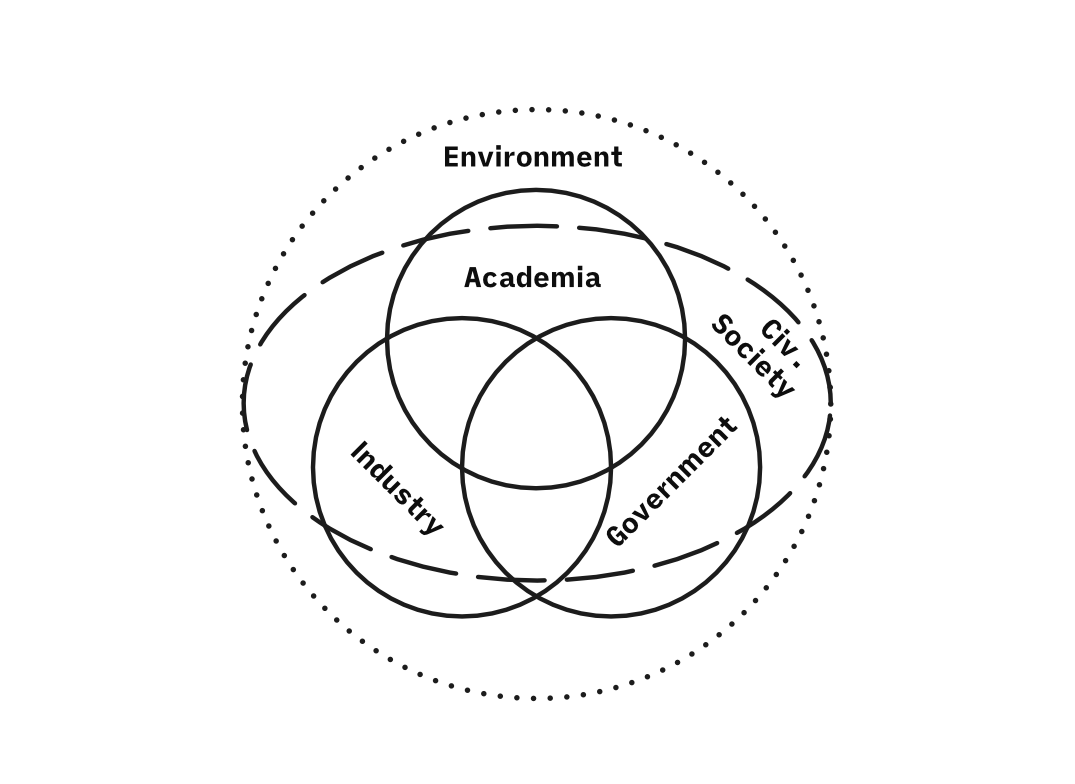
\includegraphics[width=0.5\textwidth]{figures/5.23.png}
    \caption[Spherical SIVC in DfST]{ \textbf{Spherical SIVC in DfST}. This figure is based on the “Floke programme and quadruple helix for stakeholder inclusion” in Kjøde \citep[p. 125]{kjode_entanglement_2024}
}
    \label{f5.23}
\end{figure}




\begin{figure}[h!]
    \centering
    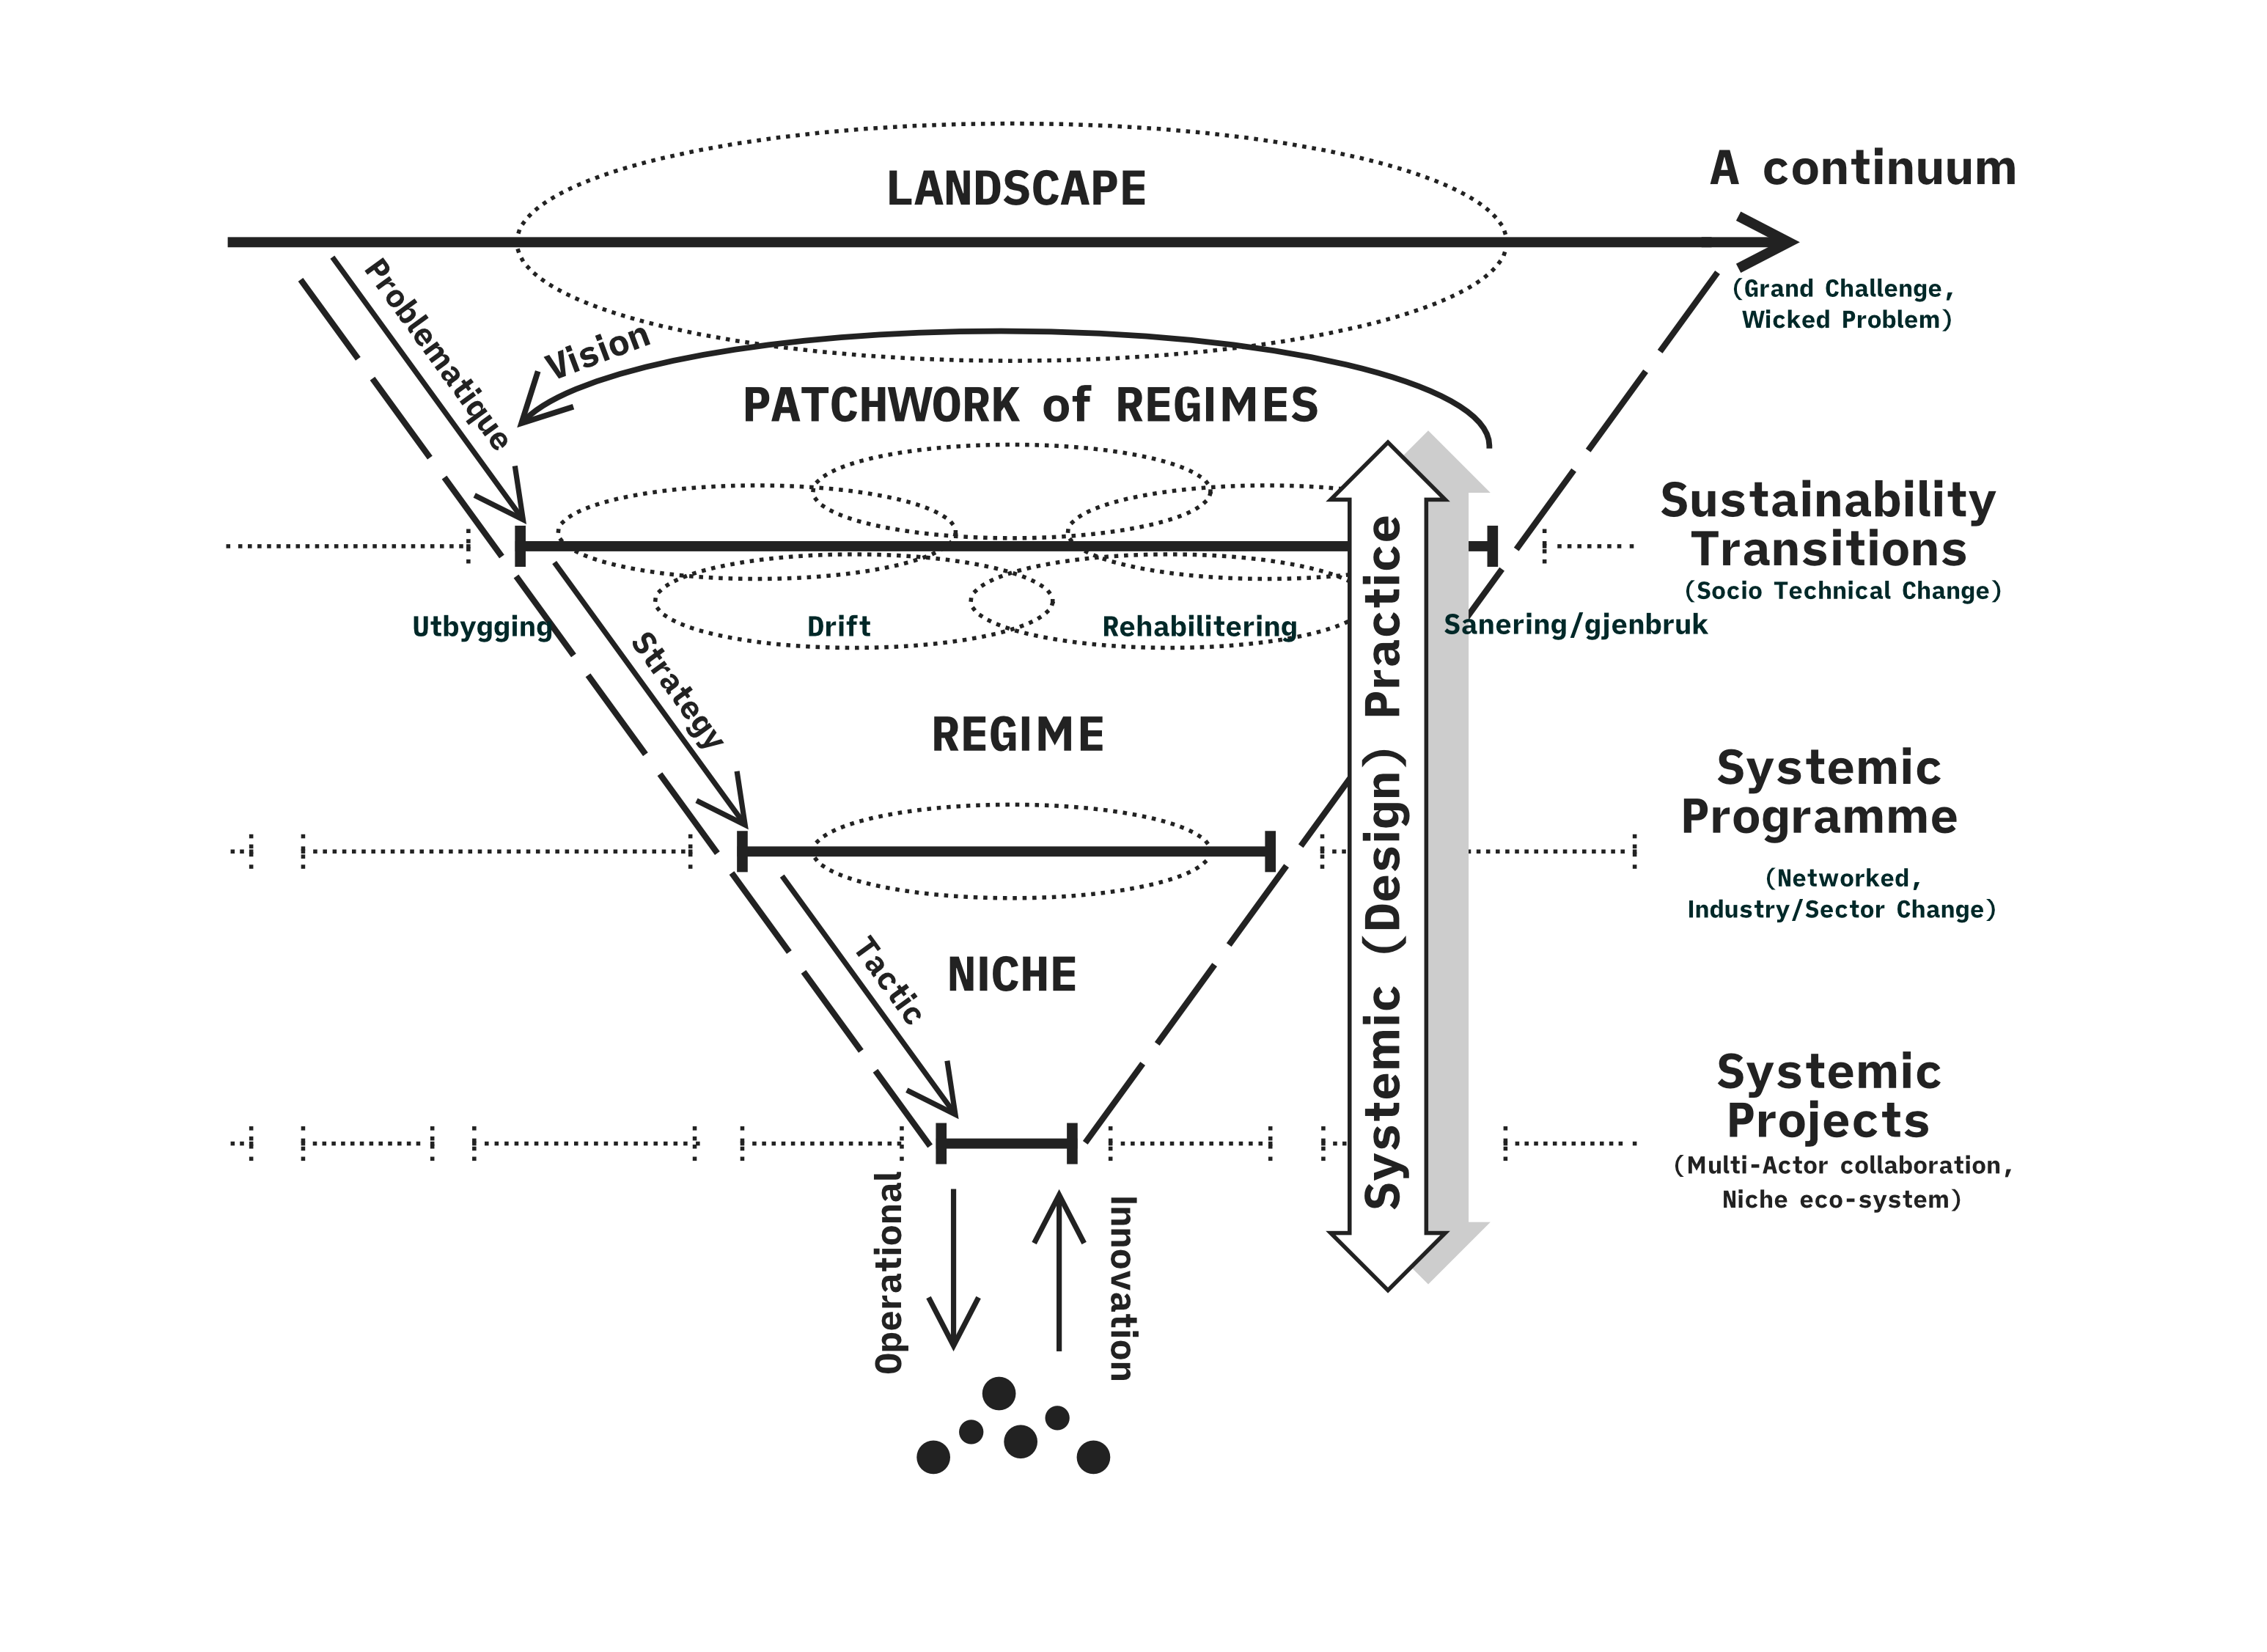
\includegraphics[width=0.5\textwidth]{figures/5.25.png}
    \caption[Conical SIVC in DfST]{ \textbf{Conical SIVC in DfST.} This figure is based on Kjøde’s “Relating systemic design practice to socio-technical systems theory and the MLP” \citep[p. 123]{kjode_entanglement_2024}. This figure includes Norwegian terms left of “Sustainability Transitions” to indicate the “patchwork of regimes” in overlapping aspects of “Socio Technical Change”: utbygging, drift, rehabilitering, sanering, and gjenbruk: 
\begin{itemize}
    \item Utbygging refers to the initial “development” \citep{cambridge_university_press_utbygging_nodate}.
\item Drift refers to the ongoing operations and management \citep{cambridge_university_press_drift_nodate}. 
\item Rehabilitering refers to the “rehabilitation” or restoration and upgrading of existing structures  \citep{cambridge_university_press_rehabilitering_nodate}.
\item Sanering refers to “clearing” or sanitation \citep{cambridge_university_press_sanering_nodate-3}.
\item Gjenbruk refers to reusing or recycling \citep{cambridge_university_press_gjenbruk_nodate}.
\end{itemize}
}
    \label{f5.25}
\end{figure}





\begin{figure}[h!]
    \centering
    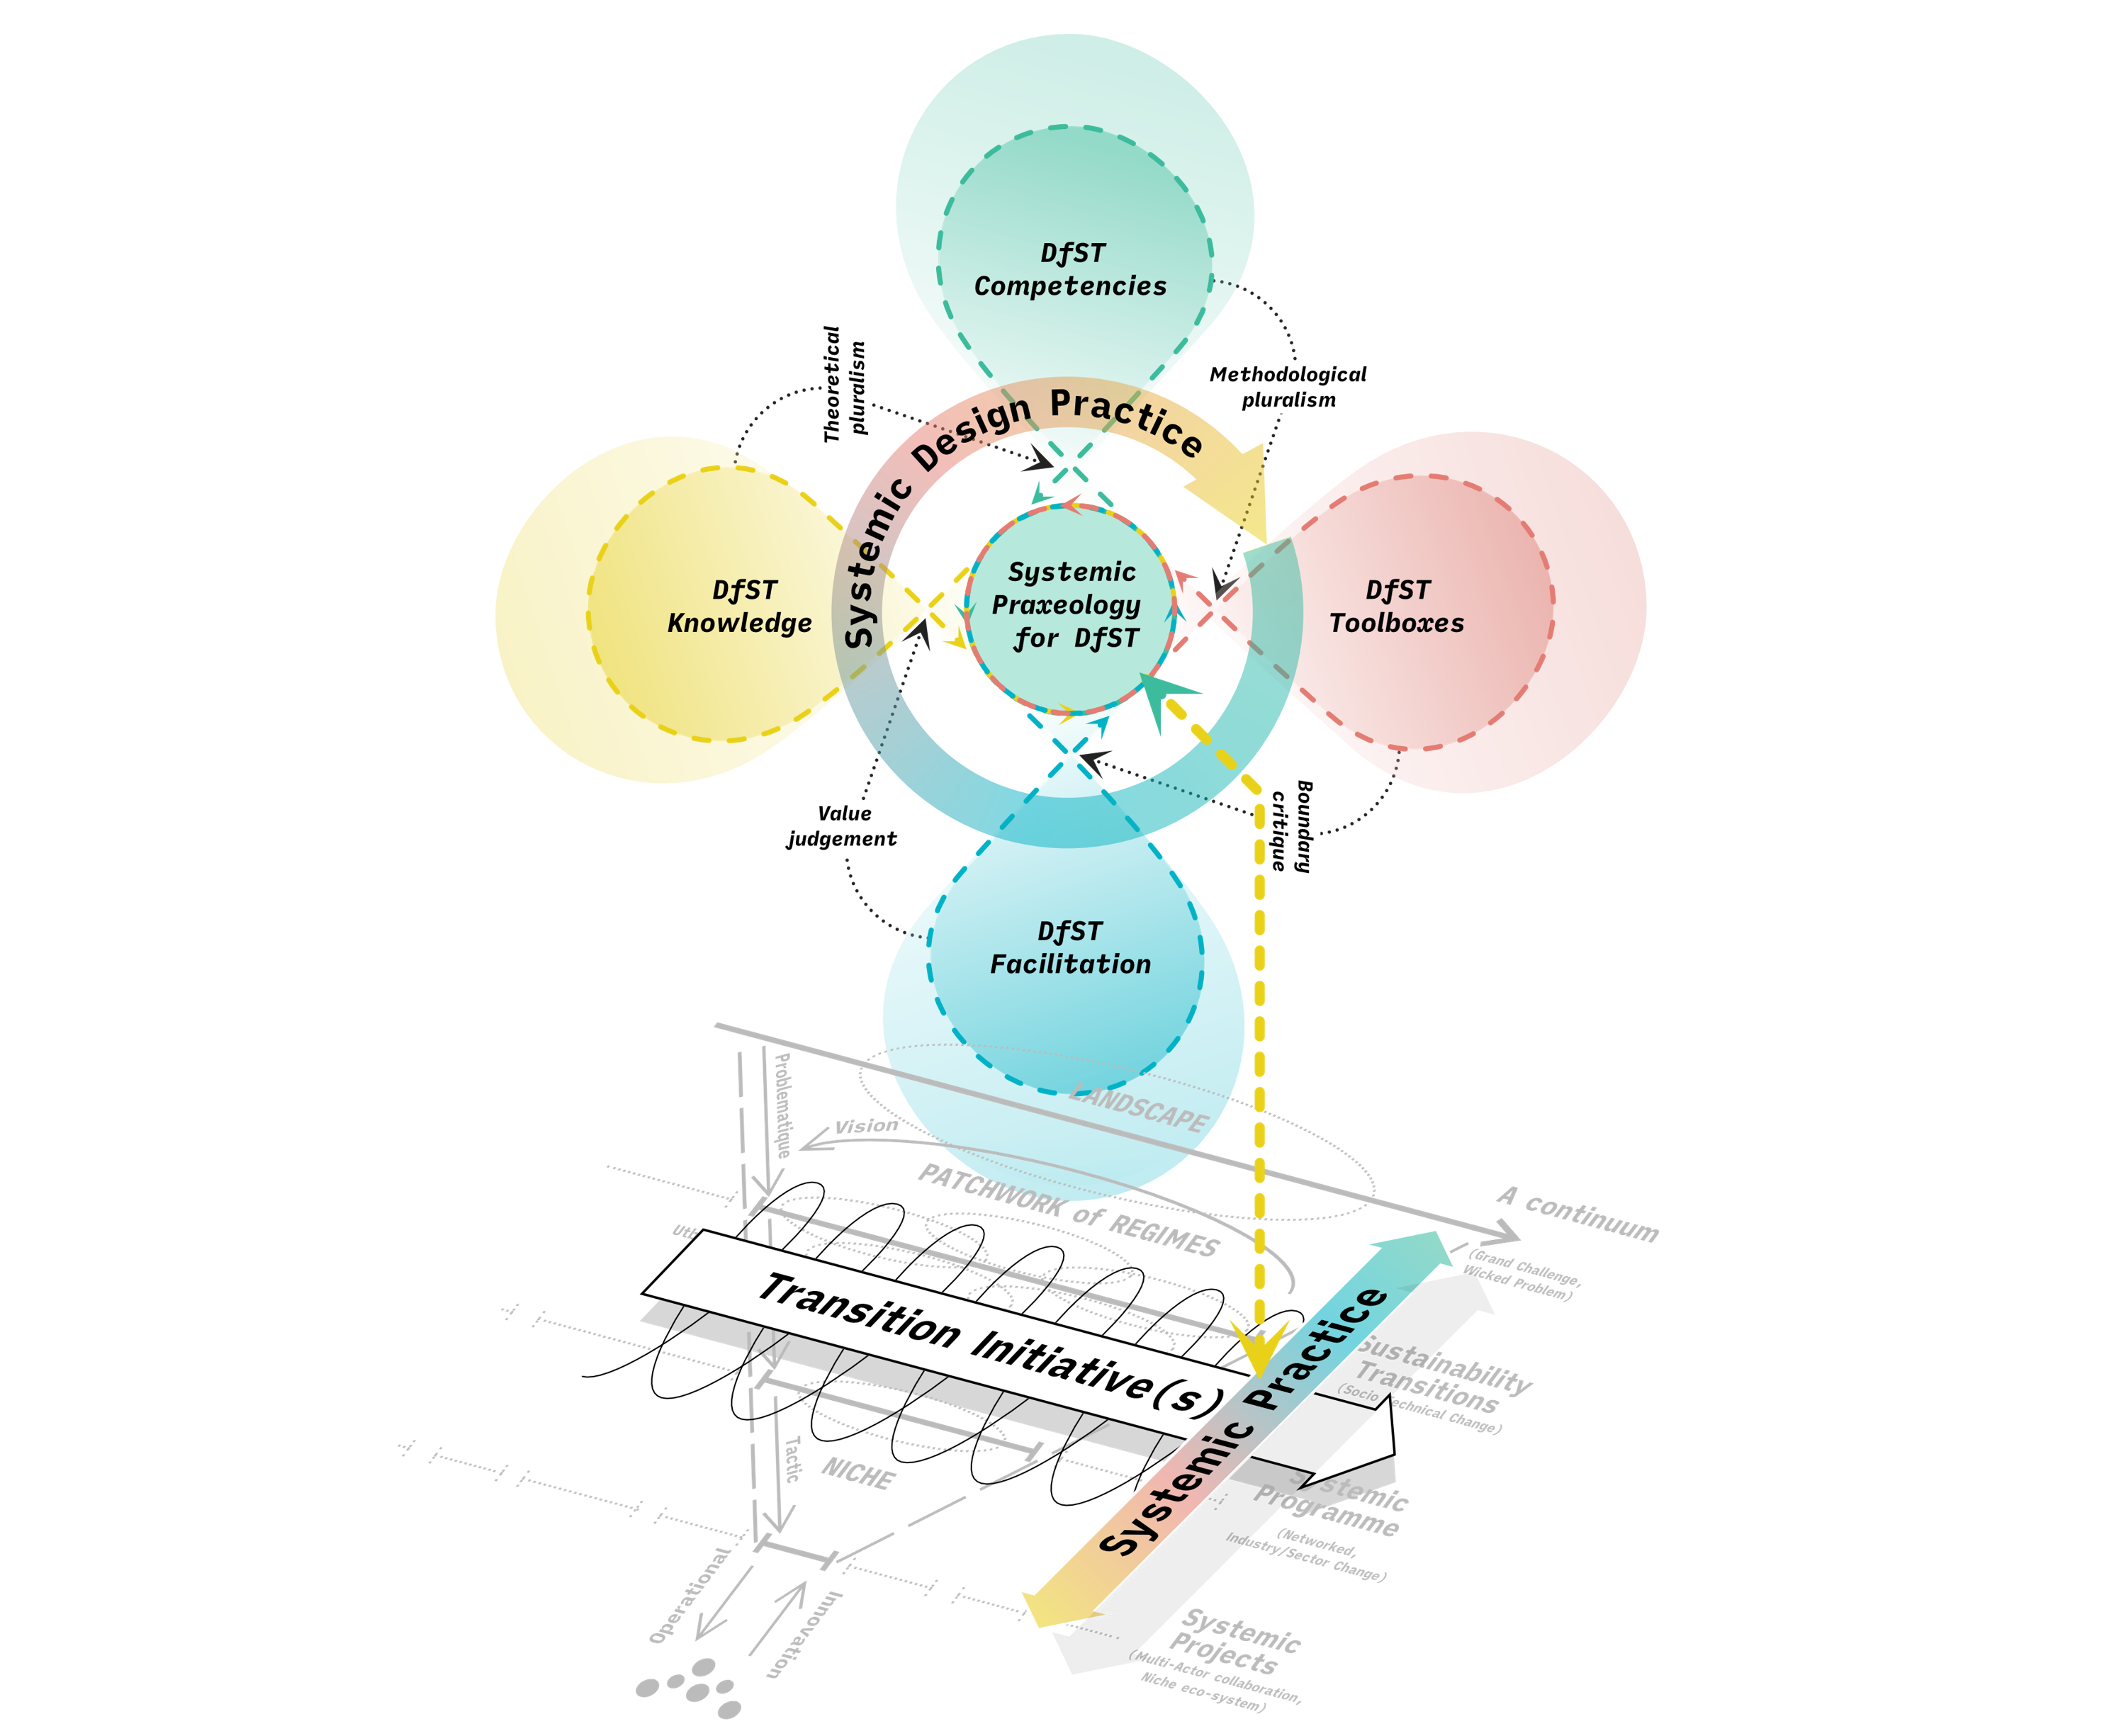
\includegraphics[width=\textwidth]{figures/5.27.png}
    \caption[Cylindrical SIVC in DfST]{ \textbf{Cylindrical SIVC in DfST.} This figure is based on Kjøde’s “Praxeological framework for DfST relating to systematic transition initiatives” \citep[p. 144]{kjode_entanglement_2024}.
}
    \label{f5.27}
\end{figure}




\begin{figure}[h!]
    \centering
    \includegraphics[width=\textwidth]{figures/5.28.Kjode b.png}
    \caption[Query Isomorph \textit{i} positioned onto DfST Systematic Combining gigamap as Cylinder Semantic Form]{ \textbf{Query Isomorph \textit{i} positioned onto DfST Systematic Combining gigamap as Cylinder Semantic Form. Evidence of DfST as source of Cylinder Semantic Forms ready for Query Isomorph analysis. Systematic Combination figure overlaid onto my cylinder network graph} Semantic Form is based on Kjøde’s “Praxeological framework for DfST relating to systematic transition initiatives” \citep[p. 144]{kjode_entanglement_2024}.
}
    \label{f5.28.Kjode b}
\end{figure}
\FloatBarrier  
\index[people]{Kjøde, Svein Gunnar}
\index[terms]{gigamapping}
\index[terms]{Systematic Combining (SC)}




\subsubsection{LLM as Sphere Semantic Form}
\FloatBarrier  
\begin{figure}[h!]
    \centering
    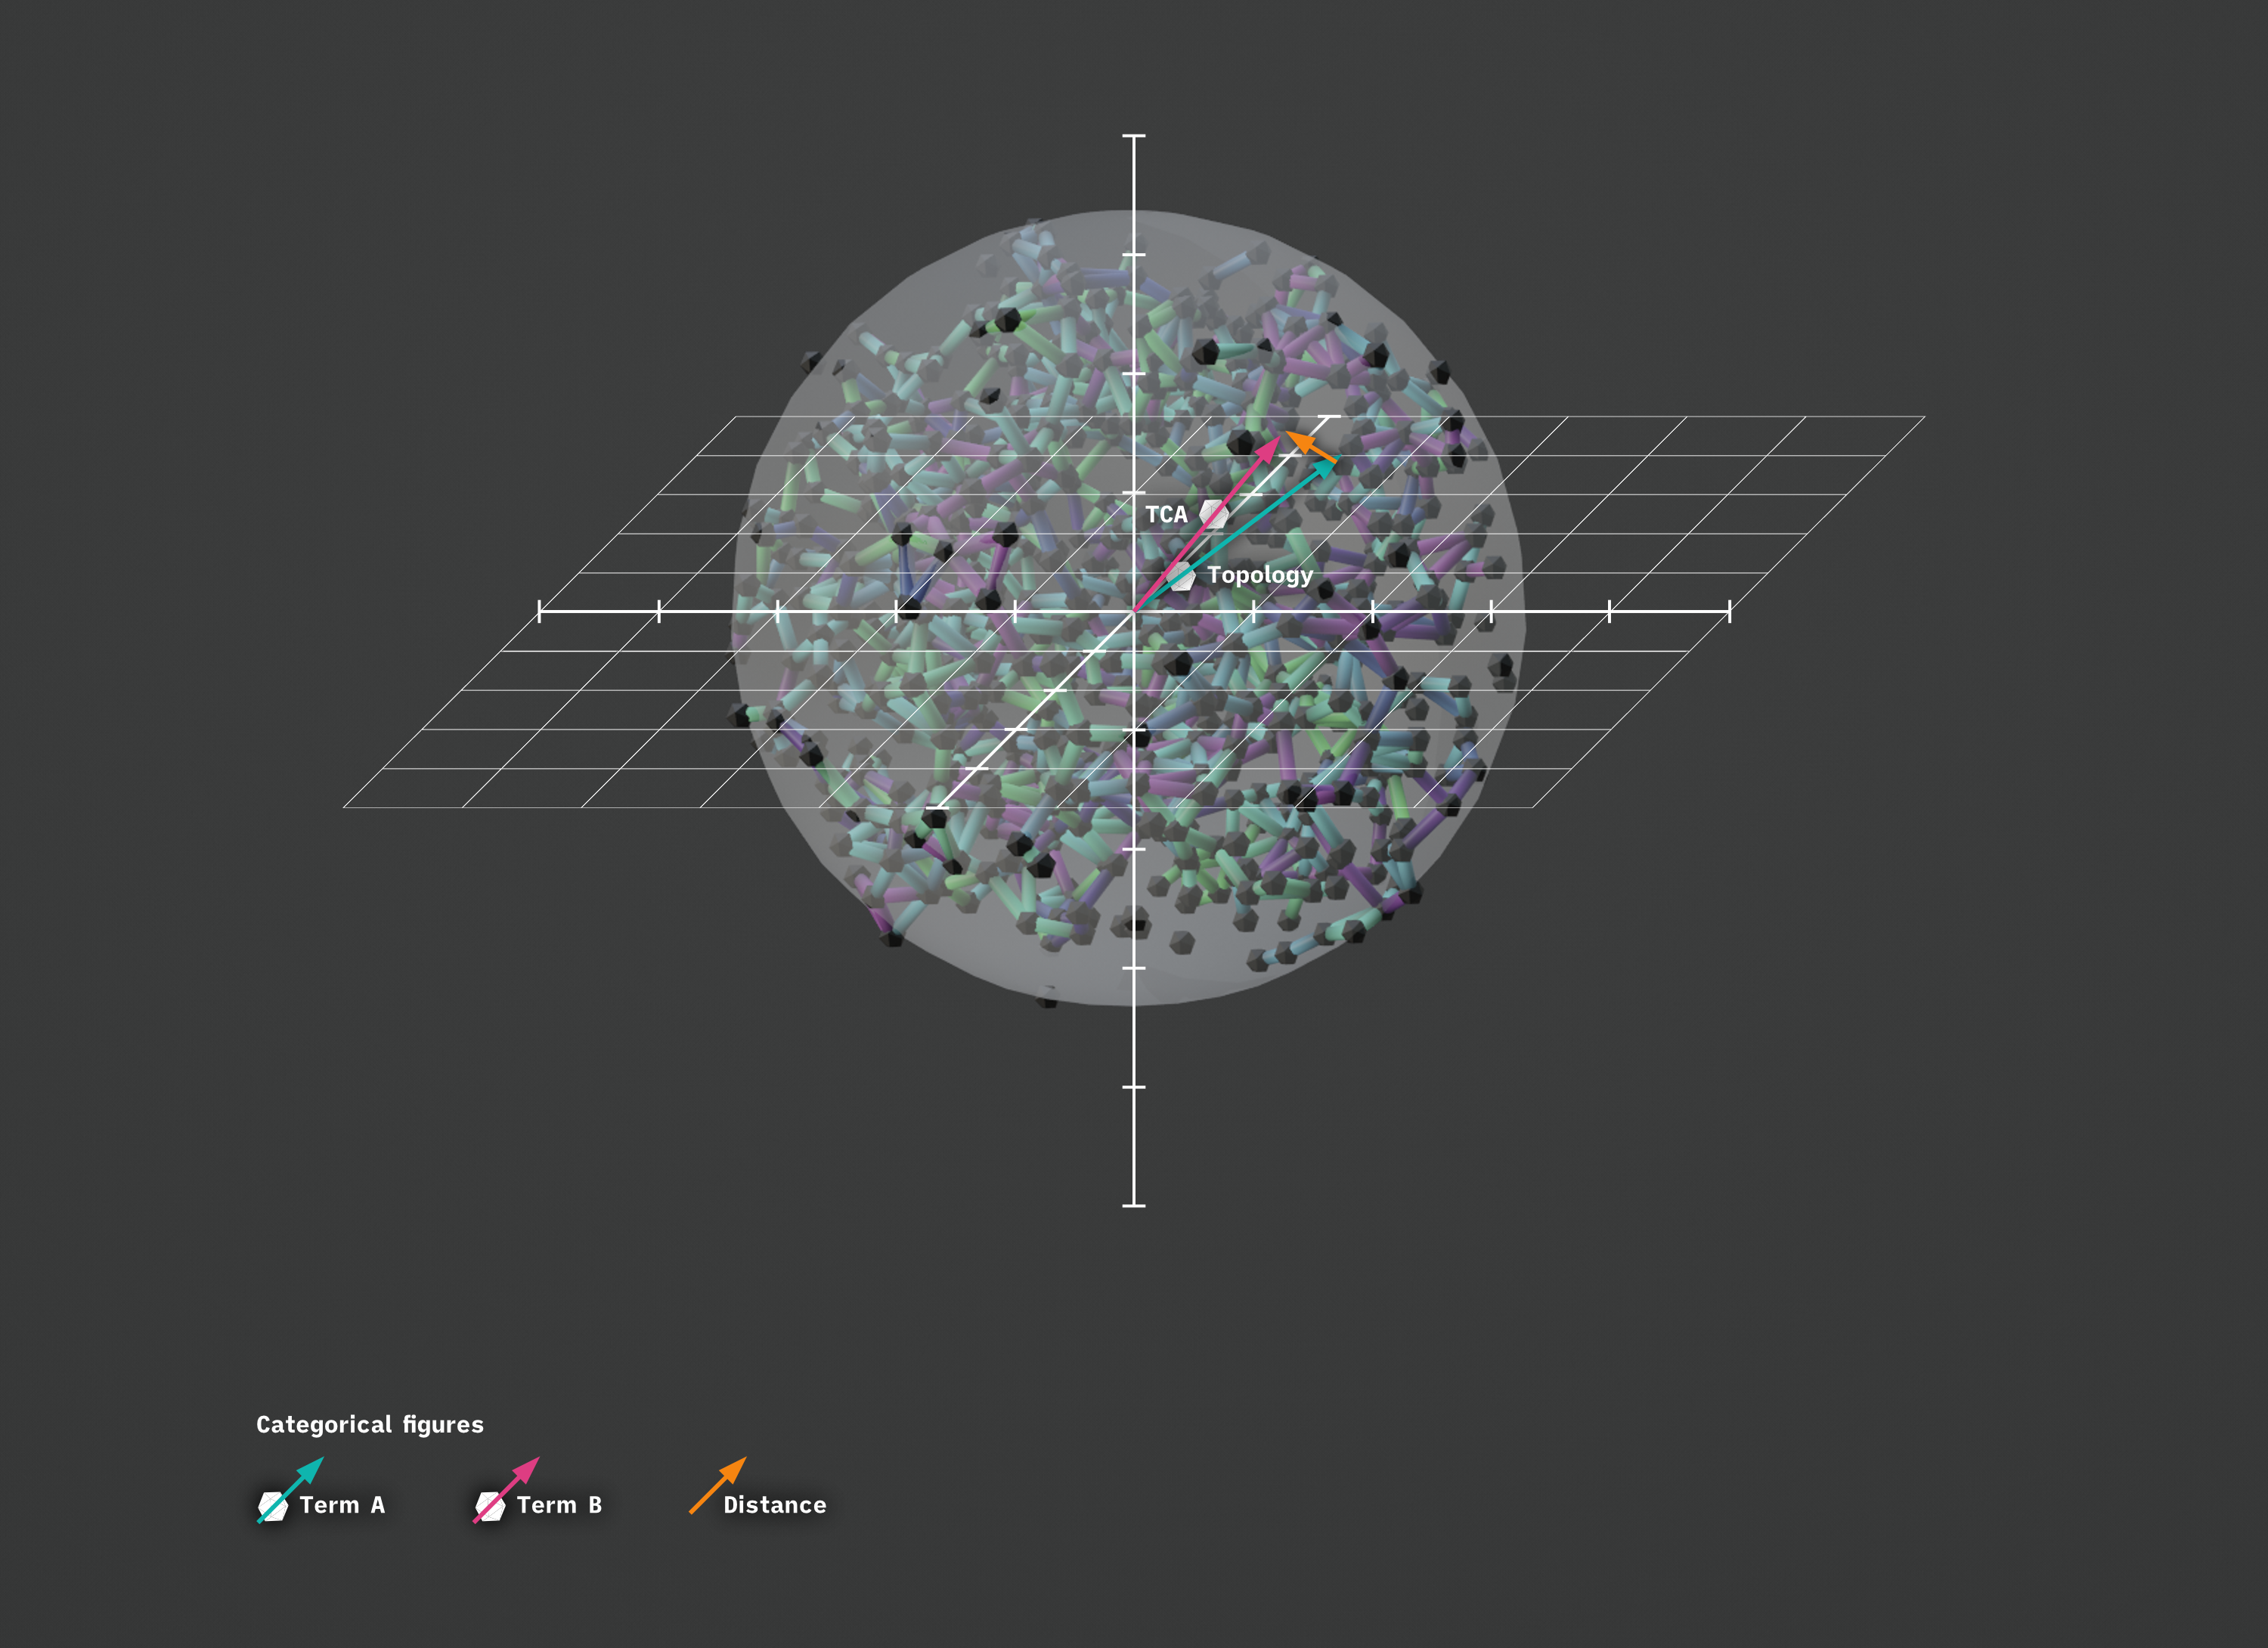
\includegraphics[width=\textwidth]{figures/5.15.Sphere LLM.png}
    \caption[Sphere Semantic Form as LLM Vector Embeddings]{ \textbf{Sphere Semantic Form as LLM Vector Embeddings.}
}
    \label{f5.15.Sphere LLM}
\end{figure}
\FloatBarrier  

Although LLMs can rely on graphs of text, such as vector embeddings, they are not intended as information visualization because for a model to be usable as AI it needs to be high-dimensional and embed thousands of dimensions. LLM vector graphs are then beyond visuospatial representation, in that they cannot be seen or captured spatially, at least not without compromising the semantic value of its dimensional interrelationships by using dimensionality reduction.

I turn here to a case study of Grant Sanderon’s illustrations of vector space which show how LLMs organize ideas as radii around a central origin point \citep{sanderson_attention_2024}. Vector embeddings operate as the direction of a line-or vector-in space; but, individual node positions work differently. However, specificity of a vector still allows for graphing individual coordinates, though variable, with the use of topology which is less concerned exact coordinates. Query Isomorphs are compatible with the LLM vector graph; for the sake of UI, Query Isomorphs may be input as individual points, but searched along vector lines within an LLM. In this way the LLM is not only an example of a Sphere Semantic Form, but a prospect for querying for Query Isomorphs within texts or groups of texts. This treatment of LLM vector graphs opens up interoperability with network graphs, and their spherical composition can be represented and leveraged as a Semantic Form.
\index[terms]{Large Language Model (LLM)}



\subsubsection{Section conclusion}

I propose that by using Systematic Combining and other forms of Systemic Design in the Design for Sustainability Transitions (DfST), Kjøde and I are engaging in a Systemic Design for Sustainability Transitions (SDfST). However, building on Pangaro, TCA Workspace is a  ``Conversation to Design the Designing" \citep[p. 185]{pangaro_design_2011}. By proposing the design of a computational expansion of SDfST, and by using meta-Systematic Combining, my work is, then, Meta-design of SDfST.
\index[terms]{Systemic Design} \index[terms]{Design for Sustainability Transitions} 
\index[people]{Pangaro, Paul} \index[terms]{TCA Workspace} \index[terms]{Systematic Combining (SC)}

As a member of the Systemic Design Association (SDA), I have witnessed the rising popularity of Systems Oriented Design and Systemic Design with the use of gigamaps \citep{sevaldson_giga-mapping_2011,sevaldson_designing_2022}. As a student at OCAD University’s Digital Futures program, I have witnessed the increased use of virtual three-dimensional visualization in game and interface design, and LLMs. Spaces with a codified practice like Systems Oriented Design and Systemic Design would benefit from a self-awareness of composition forms as a means of widening its practitioner base, and are poised to benefit from the application of LLM-assisted mathematical approaches to graph analysis like TDA and TCA.


Semantic Forms, Query Isomorphs, and TCA Workspace represent the ways my work is a visuospatialization of theory. Semantic Forms emerged from my survey of symbols, Query Isomorphs are a means of examining isomorphologies within the Semantic Form isomorphs, and TCA Workspace is a means to incorporate both Semantic Forms and Query Isomorphs within the larger practice of codifying three-dimensional modes of Visuospatial Knowledge Activation.
\index[terms]{Knowledge Activation (KA)} \index[terms]{Semantic Forms} \index[terms]{Query Isomorphs} \index[terms]{Visuospatial Knowledge Activation (VKA)} \index[terms]{TCA Workspace}






\section{From visuospatial models to theory and method}
The following contributions are ways my visuospatial models inform my theoretical and methodological proposals that build on my literature review: C3. Ontological Semantic Network Summary (OSNS), C4. Symbol-setting, C5. Terroir of Text and Graphs (TTG), and C6. TCA Researcher Grouping. 

\subsection{Contribution 3. Ontological Semantic Network Summaries}
\begin{enumerate}
     \item[\textbf{C3}] \textit{Ontological Semantic Network Summaries (OSNS)} as a means of revealing ontological relationships between ideas in a given body of research using HITL CATG, HATG, or both.

\end{enumerate}

It is considering the significance of Tree of Porphyry that I propose Ontological Semantic Network Summary (OSNS) as a framework for human-in-the-loop semantic network mapping of ontologies in an LLM or group of texts. Developing such summaries would assist researchers in identifying the inheritance of key ideas in the logic of a text or body of texts as a tool to categorize texts from a pool of references.
\index[terms]{Large Language Model (LLM)}

The operationalization of OSNS would accelerate the choice of research resources ranging from individual articles to groups of texts and Large Language Models. The graphic simplicity of the Tree of Porphyry offers an entry point for more complex representations that integrate the insights of this and other studies. For instance: three-dimensionality to accommodate more nodes, quantification of nodes and vectors to indicate more or less influence of a particular idea, the analysis of degree-difference among vertices, Query Isomorphs using Topological Capta Analysis and small graph chunks, Semantic Form configuration to reveal semantic composition, TTG to examine text in relationship to its place, further Symbol-setting in culturally-located summaries of insights, and discovering alignment between researchers in universities and among other research organizations.

As an example of a more complex OSNS I offer the following graph. It benefits from the distinctly Aristotelian orientation of both Sowa and Adler, but serves as an example of Ontological Semantic Network Summaries nonetheless.
\index[people]{Sowa, John F.}
\index[people]{Adler, Mortimer J.}
\FloatBarrier  
\begin{figure}[h]
    \centering
    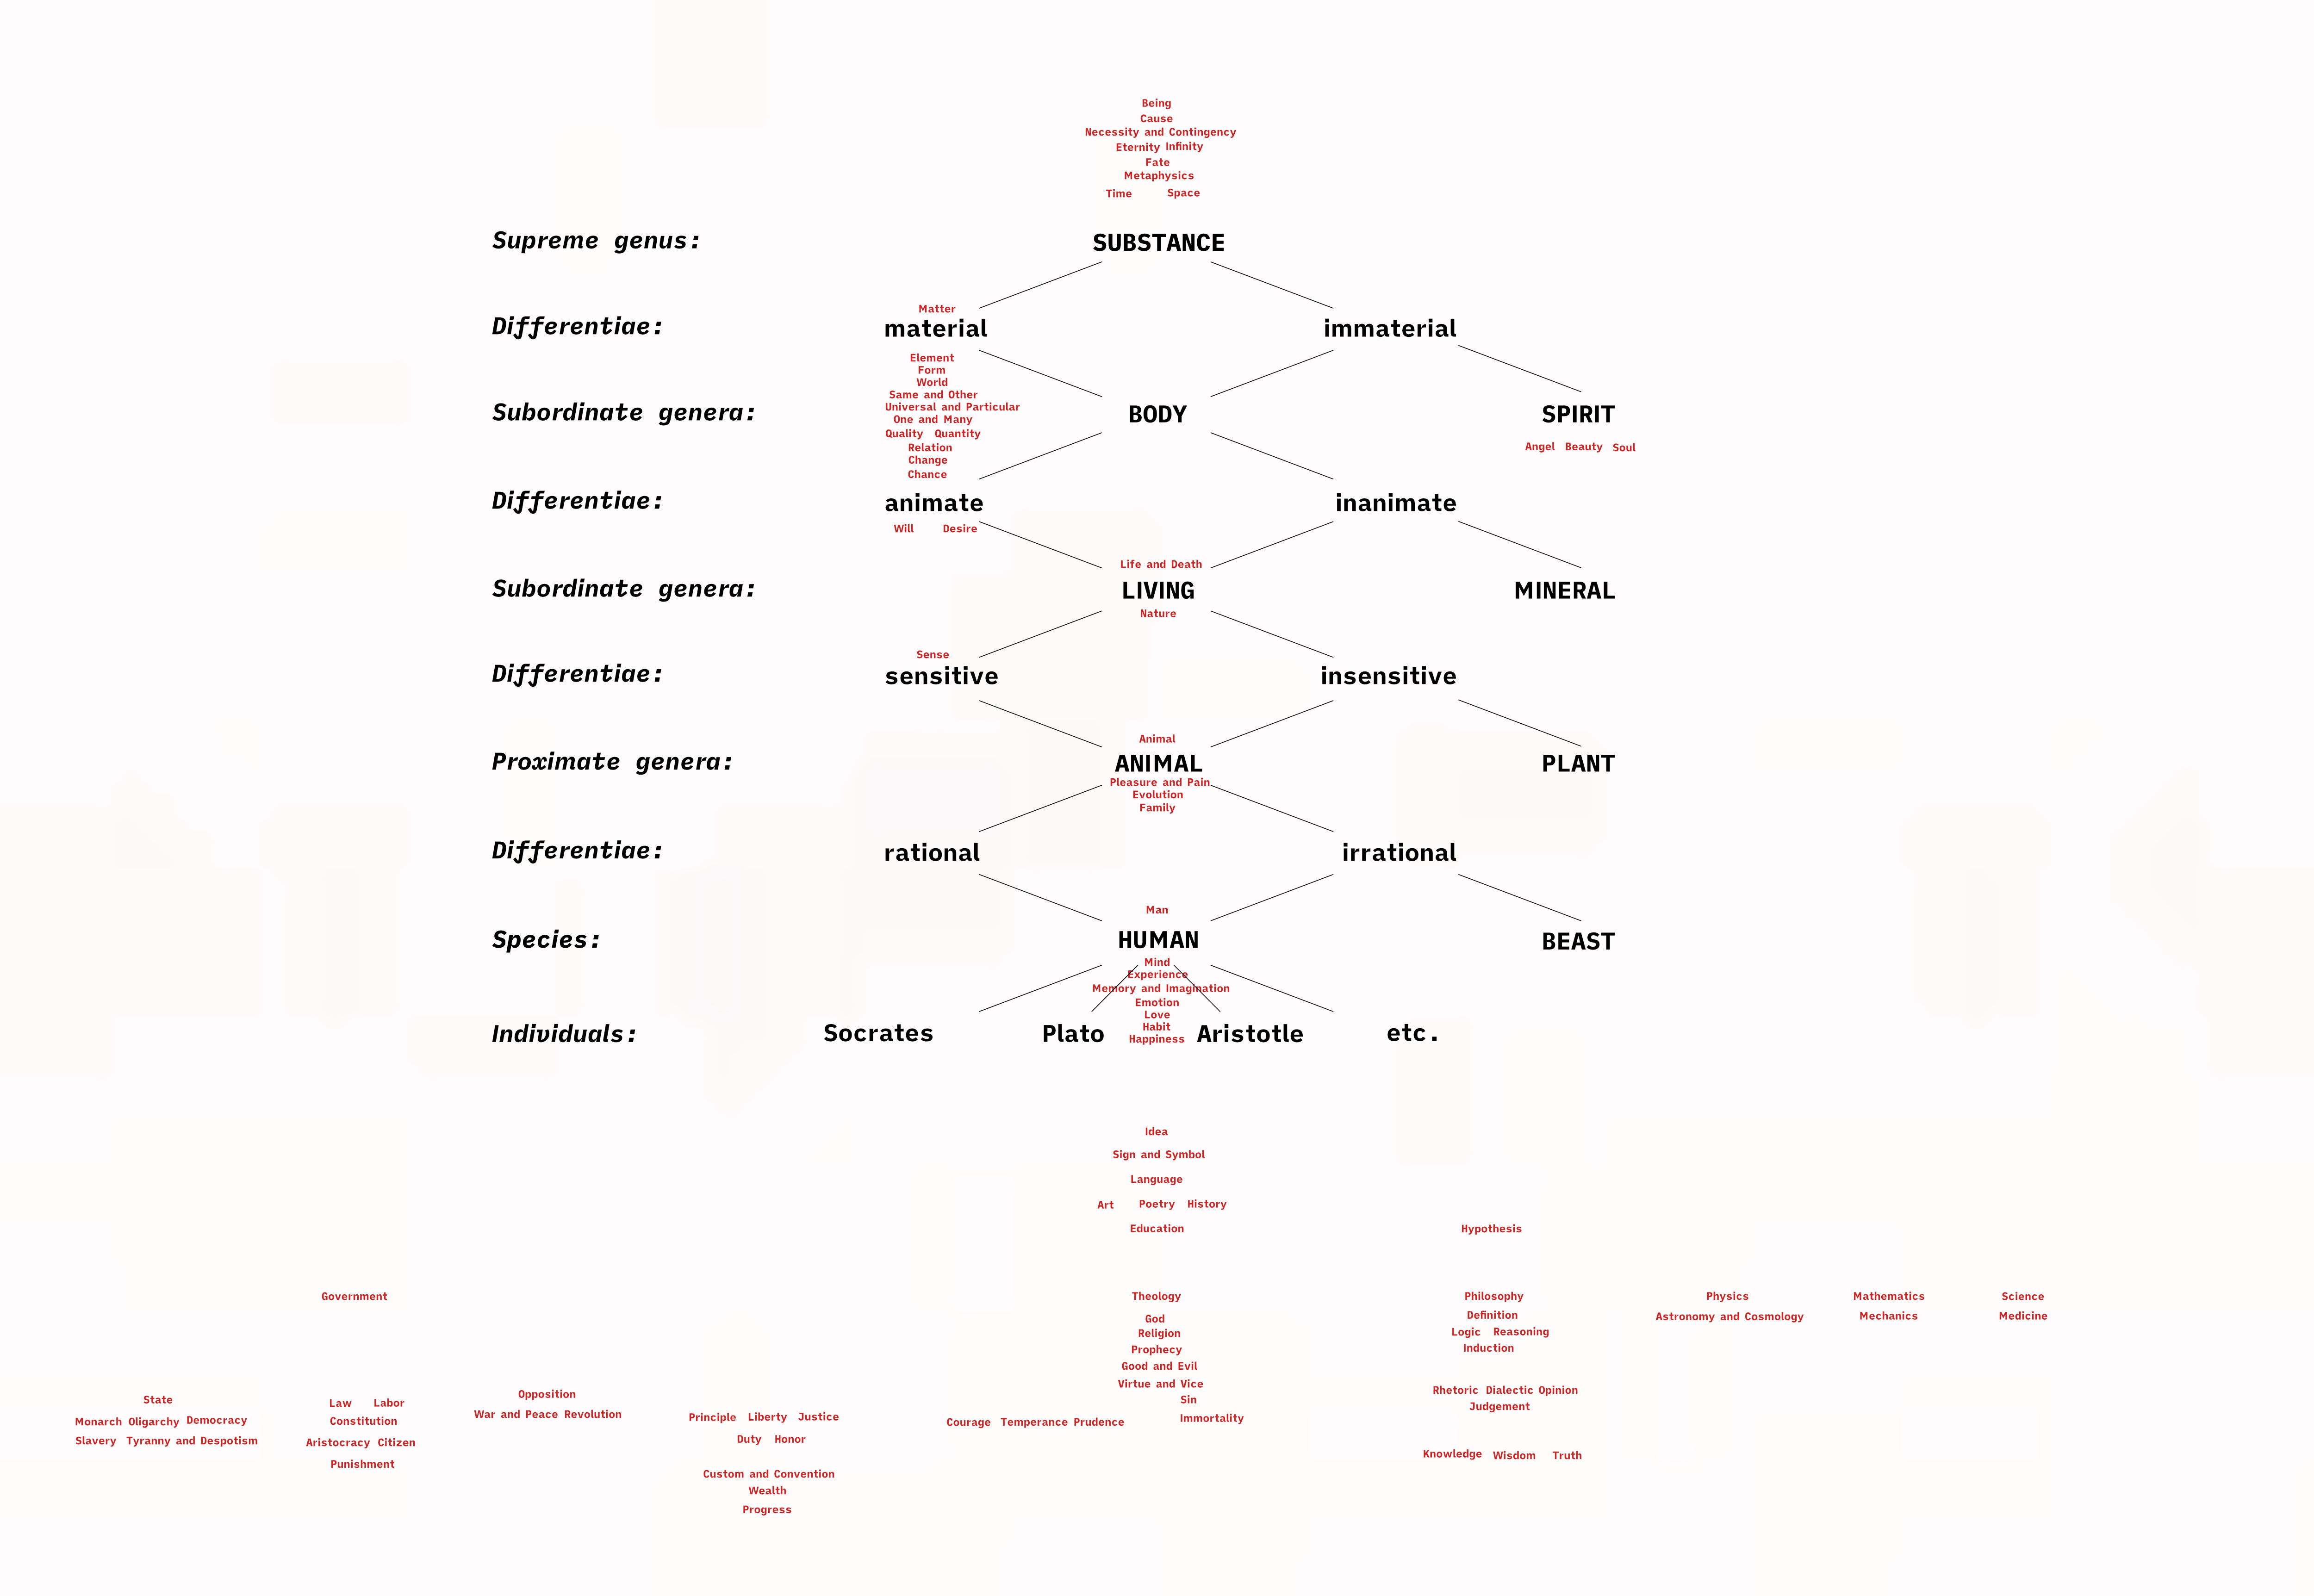
\includegraphics[width=\textwidth]{figures/6.1.png}
    \caption[An Ontological Summary Graph of the Syntopicon’s Great Ideas onto the Tree of Porphyry]{\textbf{An Ontological Summary Graph of the Syntopicon’s Great Ideas onto the Tree of Porphyry}}
    \label{f6.1}
\end{figure}
\FloatBarrier  


\subsection{Contribution 4. Symbol-setting}
\begin{enumerate}
        \item[\textbf{C4}] \textit{Symbol-setting}, a method for expanding the semiotic range of knowledge production using symbol co-creation in HITL CATG, HATG, or both.
\end{enumerate}
The relationship between word and symbol is fluid and dynamic, so a treatment of approaches that use symbols in KA follows. Symbol-setting is my proposed framework to expand word-based definition to include visuospatial modalities of symbolic co-production. 

Carl G. Liungman (or in other texts Ljungman) categorized the composition of a wide array of symbols from a variety of cultural contexts and academic disciplines in Thought Signs (1995)\footnote{Liungman categories are more intricate, but they generally group symbols by symmetry, openness, straightness of line, and the crossing of lines. \citep[p. 49-93]{liungman_thought_1995}.}. While Liungman does include symbols from outside of Europe, and in a similar vein to Adler’s work, these symbols center Western intellectual tradition. I do not propose Liungman’s work as a universal categorization, but as a starting point for the practice of categorizing the composition of symbols that informs collaborative co-production of symbols. 
\index[people]{Adler, Mortimer J.}
\index[people]{Liungman, Carl G.}

The practice of Symbol-setting can benefit from a wide variety of practices in the search of representing a community’s perspective. Branding, which might come to mind to the reader first in a design context, lends itself with a variety of tools and research approaches for the production of symbols. Gigamapping \citep{sevaldson_giga-mapping_2011} and Systematic Combining \citep{kjode_entanglement_2024} are already a kind of symbolic co-production through the use of graphs, and are thus a form of Symbol-setting. Additionally, they lend themselves to Symbol-setting through co-creating Liungman thought signs that integrate an idea or a combination of ideas into a glyph. Symbol-setting already happens to a degree in making pictographs, UX icons, and emojis. The production of symbolic objects physically or virtually makes Symbol-setting a visuospatial aptitude, and not just a visual one. 
\index[people]{Sevaldson, Birger}
\index[people]{Kjøde, Svein Gunnar}
\index[terms]{Systematic Combining (SC)}
\index[people]{Liungman, Carl G.}
\index[terms]{gigamapping}


The historical significance of symbols or “thought signs” \citep{liungman_thought_1995} is vast, and can take on a great deal of cultural seriousness, so I do not propose the process of symbolic co-production lightly. In fact I propose that Symbol-setting can be hierophanic, and be part of a community’s understanding of the manifestation of the divine or transcendent, introduced in my critical discussion of Eliade \citep[p. 11]{eliade_sacred_1987}.
\index[people]{Liungman, Carl G.}
\index[people]{Eliade, Mircea}

I believe that the visuospatial co-prouction of the symbol itself is underdeveloped in the design space, systemic and otherwise. Pangaro’s conversational model of co-evolutionary design for narrowing and expanding language \citep[p. 185]{pangaro_design_2011} and ECCD “language setting” \citep[p. 8-9]{creative_reaction_lab_equity-centered_2018} can both benefit from Symbol-setting. By providing new ways for arriving at common understanding, TCA Workspace facilitates conversations across academic difference and power difference by empowering equity-oriented approaches like ECCD.  
\index[terms]{TCA Workspace}
\index[people]{Pangaro, Paul}

By proposing Symbol-setting I aim to support co-creative KA that uses more interpretative facets of visuospatial epistemology in the production of “thought signs” \citep{liungman_thought_1995}. When practiced in TCA Workspace, Symbol-setting takes the forms, and hyper-forms, of multidimensional text analysis and expands the capabilities of various design practices.
\index[terms]{TCA Workspace}
\index[people]{Liungman, Carl G.}
\index[terms]{visuospatial epistemology}



\subsection{Contribution 5. Terroir of Text and Graphs}
\begin{enumerate}
        \item[\textbf{C5}] \textit{Terroir of Text and Graphs (TTG)}, a method of HITL CATG that uses TCA to interpret and reveal semantic relationships between (a) texts and graphs, and (b) the features and systems of ecological place.
\end{enumerate}
\FloatBarrier
\begin{figure}[h]
    \centering
    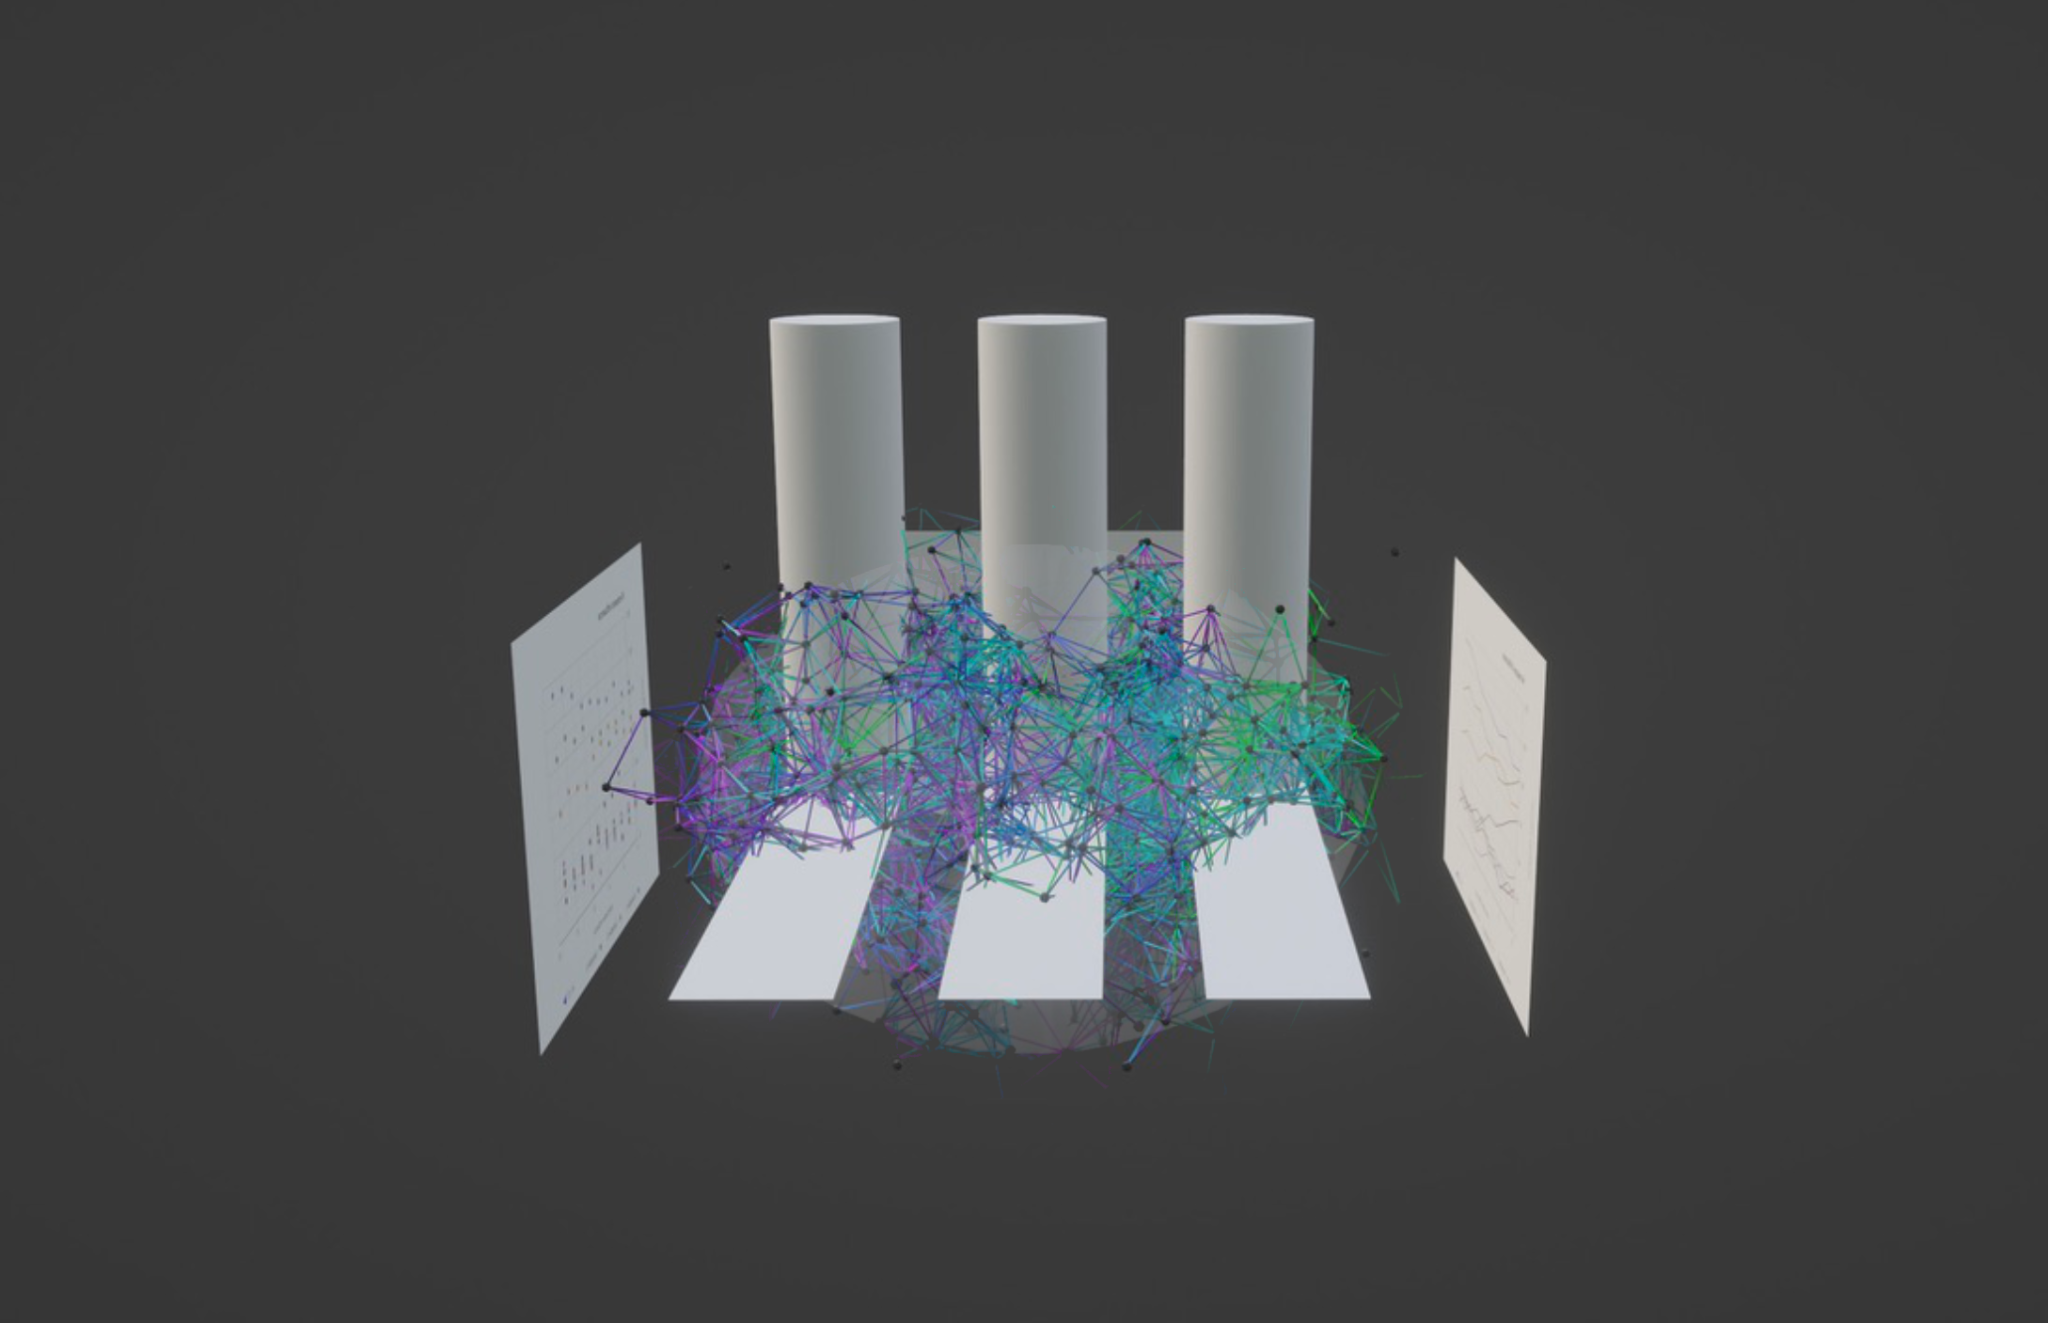
\includegraphics[width=\linewidth]{figures/6.2.png}
    \caption[Torus vs Silos]{\textbf{Torus vs Silos.} Illustration of spatial gigamap format with Horn Torus Semantic Form of text network graph. This example visualizes an analysis of three siloed hyper-specialized work "communities" and three agricultural monoculture operations nearest to them in the same province or municipality. This model proposes an inter-applicable systems analysis to identify multi-solutions between siloed over-work and extractive agriculture.}
    \label{f6.2}
\end{figure}
\index[terms]{Horn Torus Semantic Form}
\index[terms]{gigamapping}
\FloatBarrier

I first learned about wine from my father, who taught my brother and I how to taste for region. It is from viticulture that I borrow the term terroir, where the term is used to relate “the sensory attributes of wine to the environmental conditions in which the grapes are grown”, which involves considering interacting factors like “climate, soil, cultivar, and human practices” \citep[p. 1]{van_leeuwen_concept_2006-1}. The interaction of ecological factors is at play in making text and graphs too, so I propose TTG. 

The relationship between place and language influences fundamental characteristics of how we think. To apply Tversky’s research on the neuroscience of the visuospatial one might examine differences in metaphor to the verticality and horizontality of place, one would expect the semantic value of verticality would differ considerably between communities living in perilous high altitude when compared to communities living near sea-level. To take another example from India, the rounded wavy lines that characterize many scripts are “usually explained as a result of the exigencies of writing with a stylus on palm leaves” \citep[p. 39]{salomon_indian_1998}. Of course, many other types of relationships between place and language exist. So, I propose TCA as a method to better understand the relationship between the ecological and conceptual as a means of improving the translation of information from one ecologically-located discipline or tradition to another. In ecological TCA I propose that we can expect a ‘terroir’ of text and graphs, or characteristics of a particular thought tradition which align themselves with characteristics of their place. 
\index[people]{Tversky, Barbara}

Examining the relationship between place and idea using TCA has significant implications for our understanding of contemporary classifications of city, country, and wilderness. In the following figure, Illustration of spatial gigamap format with Horn Torus Semantic Form of text network graph, I propose that rewilding as a means of ecological diversity in food supply can consiliently inform the diversification of interdisciplinary forums in academic settings. Such a model would derive insight from solutions in sustainable food-production, which assuage the ecological costs of agricultural monoculture. Applying said solutions to siloed hyper-specialized over-work would benefit from more opportunities for disciplinary inter-pollination as an improvement on the current monoculture of work. These and other such entry points to relief via systemic analysis can be expected from developing Topological Capta Analysis into a wider de-siloing practice where text is examined in relation to frameworks from within and without its discipline of origin. 
\index[terms]{Horn Torus Semantic Form}
\index[terms]{gigamapping}

Developing a TCA practice to understand TTG would go on to address gaps that were not covered in this study, namely empirical gaps and spatial gaps. Empirically, we would be able to collect data or create capta to fully understand text terroir through data model experiments. Spatially, understanding the relationship between text and place is limited compared to what can be achieved with a text terroir analysis. Expanding research on Query Isomorphs using TCA and TTG would provide a new means of articulating interregional relationships in ways that could empower underrepresented areas. If adjoined to Indigenous approaches to Artificial Intelligence, TTG can bolster new technologies for climate justice and resilience.

My model TTG model \textit{Torus vs Silos} illustrates the way Topological Capta Analysis can map relationships between ecological systems and information systems using Semantic Forms, Query Isomorphs and visuospatial gigamapping. More specifically, \autoref{f6.2}  visualizes an analysis of three siloed hyper-specialized over-worked groups of people and three extractive agricultural monoculture operations nearest to them. Using TTG in this way, I  would seek to reveal parallels of extractive capitalism that are at play in both ecological space and idea space in order to support their transition into more anthropo-symbiotic\footnote{The term "anthropo-symbiotic is borrowed from Fonseca et al.'s \textit{Anthropo-symbiotic ethics: a path to the sustainability of life} which discusses ethical "theories with a more conciliatory and balanced view about the relation between the environment, humans and animals" \citep{fonseca_anthropo-symbiotic_2022}} ways of being and knowing. 


\index[terms]{Artificial Intelligence (AI)}
TTG can more explicitly delineate relationship between land and language in human and non-human ways of knowing. From an Indigenous perspective, the wisdom that is carried in story, cultural practice can be articulated through the expanded field of graphs of texts which includes Semantic Forms, Query Isomorphs and TCA Workspace in gigamaps, Systematic Combinations, topic models, and the vector graphs that form the basis of AI Large Language Models. The benefits of TTG as integration of diverse wisdom lineages, including the distinctly anthropo-symbiotic Indigenous ways of knowing, can be simultaneously an act of ecojustice and a means of informing ST. At the core of TTG is my commitment to Indigenous data sovereignty \citep[p. 12]{lewis_abundant_2024} in which "Indigenous practitioners are making the decisions that guide the development of AI themselves" \citep[p. 8]{lewis_abundant_2024}. A TTG-based HITL CATG of fields like ethnobotany, ethnoecology\footnote{Turner et al. define the interrelated fields of ethnobotany and ethnoecology \citep[p. 6-7]{turner_introduction_2020}.}, biocultural memory 
\footnote{Monterrubio-Solis et al. define biocultural memory as follows: “Biocultural memory refers to the human reliance on intergenerational relationships, not only to one another but within territories, where the physicality of agroecosystems, material and symbolic meanings, as well as institutions join to constitute biocultural memory” \citep{monterrubio-solis_narrating_2023}.}, plant-human co-evolution represents a critical part of KA.
\index[terms]{TCA Workspace}
\index[terms]{Systematic Combining (SC)}
\index[terms]{gigamapping}

\subsubsection{Land and Indigeneity}
As I reconnect with my South American Indigenous roots, buried by colonialism and xenophobia, develop computational tools for climate justice and resilience, I seek research collaborators who share these goals. 

One such initiative is the Abundant Intelligences project, an international research effort spanning Canada, the United States, and New Zealand. Jason Edward Lewis, professor of computation arts at Concordia University and the University Research Chair in Computational Media and the Indigenous Future Imaginary, is co-leading the Abundant Intelligences project. Lewis et al. assert that the way AI is developed at present is limited by "Western rationalist epistemologies that exclude many ways of knowing" so, "the systematic operationalization of bias against non-white, non-male, and non-Western peoples" is also unable to "adequately, robustly, and humanely conceptualize intelligence-much less attempt to replicate it." \citep[p. 1-2]{lewis_abundant_2024}.

The OCAD University pod for Abundant Intelligences is called the \textit{A Dish with One Spoon ––Towards “Generous AI” Invention and Collaboration} project. As the first OCAD U research assistant brought on to the team, I aim to support the research team's activities. Our team will draw upon Indigenous frameworks to offer redefinitions of intelligence, and develop computational practices that refashion AI from being a tool of "exclusion, extraction, and eradication into engines for increasing our care of one another and our world" \citep{visual_analytics_lab_abundant_2024}. 
\index[terms]{A Dish with One Spoon}

The OCAD U pod co-investigators, Dr. Sara Diamond and Archer Pechawis both worked with Cree/French Métis performance artist and theorist Âhasiw Maskêgon-Iskwêw (1958-2006), creator of \textit{isi-pîkiskwêwin-ayapihkêsîsak (Speaking the Language of Spiders)} \citep{maskegon-iskwew_isi-pikiskwewin-ayapihkesisak_1996}. Maskêgon-Iskwêw's work calls in the animist perspective of spider as maker of networks in hyperspace. In the age of AI I would love to know what Maskêgon-Iskwêw would say about the web that is itself animate: the decentralization of ideas' provenances by reason-automatons; the opportunities of using rhi-zombies with the aim of transubstantiating the poisons of ecocide, balanced with the risks of becoming its host/s in tangle of disinformation, confusion, and illusion.
\index[terms]{rhizome}
\index[terms]{rhi-zombie}

Maskêgon-Iskwêw cites from the general "principles for the development of Indigenous networked art production" that were "established at the \textit{drumbeats to drumbytes} gathering [...] at The Banff Centre from March 12 to 15, 1994, coordinated by the Aboriginal Film and Video Art Alliance": "To govern ourselves means to govern our stories and our ways of telling stories" \citep[p. 19]{maskegon-iskwew_drumbeats_2005}. If unchecked, AI will continue to exacerbate marginalization by expanding the tools of imperialism and colonization. The stakes of critical AI research like the Abundant Intelligences project are high and growing higher. 

I maintain a cautious optimism for using Large Language Models in a Two-Eyed\footnote{Two-Eyed Seeing as a principle was "advanced by Canadian Indigenous leaders, notably Mi'kmaw Elders Albert and Murdena Marshall." \citep[p. 3]{bourgeois-doyle_two-eyed_2019}} AI framework that draws strengths from both Indigenous and Western ways of knowing \citep[p. 3]{bourgeois-doyle_two-eyed_2019}. To echo Bourgeois-Doyle, I am committed to a critical evaluation of TTG to maintain a Two-Eyed Seeing model for Topological Capta Analysis, with and without AI, which works for "integrated thinking, respectful multidisciplinary collaboration, and transcending combinations of interests for public good." \citep[p. 3]{bourgeois-doyle_two-eyed_2019}. 

\subsection{Contribution 6. TCA Researcher Grouping}
\begin{enumerate}
        \item[\textbf{C6}] \textit{TCA Researcher Grouping}, a proposal to use TCA for grouping research collaborators more effectively using HITL CATG, HATG, or both.
\end{enumerate}
Developing Computational Analysis of Texts and Graphs (CATG) can improve our work relationships in research institutions. As the administrative arm of TCA Workspace, I propose TCA Researcher Grouping to manage richer databases of researchers’ work with the aim of grouping researchers more effectively. Key areas of application will be suggesting researchers for groupings that can expand the scope of projects to access larger grants, and pairing new researchers to existing teams. 

Innovating information technology for KA can improve climate resilience efforts. As a means of operationalizing CATG, TCA Workspace and TCA Researcher Grouping have the potential to catalyze solutions with more effective cross-pollination of disciplines. To apply a term from agricultural practices like permaculture, there is an element of rewilding at play. Analogous to the term “biodynamic agriculture” \citep{steiner_what_2005}, TCA Workspace and TCA Researcher Grouping are a move toward a more disciplinarily-dynamic knowledge-culture. This is rewilding on and beneath the page.
\index[terms]{TCA Workspace}